\documentclass[xcolor={dvipsnames}]{beamer}

% Paquets utilisés
\usepackage{animate} % pour faire des animations
\usepackage{listings} % pour insérer des lignes de codes avec de la coloration syntaxique
\usepackage[audience=english]{beameraudience}  % pour écrire la présentation en 2 langues
\usepackage{textpos} % pour positionner des figure où l'on veut
\usepackage{tikz} % pour faire de jolies figures
\usepackage{pifont} % pour avoir des symboles sympa

% Thème et options générales de mise en forme
\usetheme{Singapore}
\usecolortheme{rose}
\setbeamertemplate{page number in head/foot}[totalframenumber] % pour ajouter les numéros des pages
\setbeamertemplate{navigation symbols}{} % pour virer les symboles "page suivantes" ...
\makeatletter % pour avoir des puces de progression
\setbeamersize{
  text margin left = 0.2cm, % modification des marges (normalement c'est 1 cm)
  text margin right = 0.2cm}
\setbeamertemplate{block begin}{  % pour ajuster la taille des block
  \begin{minipage}{.87\textwidth}%
    \begin{beamerboxesrounded}[upper=block title,lower=block body,shadow=true]{
    \raggedright\usebeamerfont*{block title}\insertblocktitle}
    \raggedright
    \usebeamerfont{block body}}
  \setbeamertemplate{block end}
{\end{beamerboxesrounded}\end{minipage}\vskip\smallskipamount}
\setlength{\unitlength}{1cm}

% Ajout de la description du language Gibiane (pour le paquet "listings")
\lstdefinelanguage{gibiane}{
  morekeywords=[1]{
      opti, born, dens, droi, lapl, cerc, mota, oper,
      quel, inte, para, et  , poin, plus, moin, tran, lister,
      rota, trac, inve, cote, elem, cont, diff, chan, list,
      surf, conf, info, tour, homo, affi, syme, incl, elim,
      titr, racc, tass, sort, lire, bary, dall, orie, manu,
      oubl, comp, cout, pave, comm, noeu, nbel, nbno,
      noti, face, coor, norm, temp, volu, lect, sauf, prog,
      +   , -   , *   , /   , **  , flot, enti, log , exp ,
      depl, psca, pvec, pmix, liai, regl, hook, sols, reso,
      date, rigi, bloq, depi, hota, stru, text, proj, venv,
      elst, jonc, reco, mass, clst, sigm, rela, forc, mome,
      vloc, base, dime, extr, vers, vibr, maxi, xtmx, ytmx,
      >   , <   , >eg , <eg , ou  , ega , non , neg , mult,
      pjba, crit, diag, xtx , uniq, bsig, deda, max1, mots,
      ipol, abs , sin , cos ,
      atg , enve, isov, detr, enle, remp, inse, coli, tria,
      tabl, redu, symt, anti, resu, pres, exco, nomc, saut,
      defo, appu, inva, prin, vmis, ksig, sign, suit, 
      valp, ordo, tire, rege, dess, amor, char, coul, chpo,
      afco, evol, orth, thet, comb, deve, vect, pica, capi, 
      copi, dimn, sauv, rest, cara, mate, gene,
      capa, elfe, jaco, plas, gree, mode, finp, xty ,
      debp, ktan, form, mess, nnor, cubp, cubt, cer3, fdt ,
      seis, ener, epsi, intg, cour, reac, supe, zero, depb,
      exci, kp  , acti, elas, erre, cong, lump, obte,
      vari, modi, masq, exis, mini, grad, ense, ifre, dfou,
      sigs, mapp, somm, brui, rten, dspr, tfr , tote,
      graf, tres, type, osci, spo , inde, chsp,
      tagr, perm, cabl, fofi, work, qulx, debi, 
      cmoy, comt, cond, flux, rimp, filt, tfri,
      conc, iter, acqu, sour, conv, acoh, psmo, asih, ecou,
      mena, synt, argu, atah, dyne, fonc, resp, plac,
      vale, proi, exce, aret, calp, indi, act3, biot,
      dedu, conn, nloc, chai, cosi, cvol, diad, hann, insi,
      lsqf, ltl , pert, prns, psrs, siar, spon, visa, cneq,
      ccon, mesu, pile, util, menu, cosh, sinh, tanh,
      deg3, aide, racp, refe, ksof, nske, kmab,
      noel, doma, fpu , gmv , eqpr, eqex, vibc, avct,
      kdia, kmtp, kmf , mdia, dfdt, tcrr, tcnm, sqtp, somt,
      nlin, cmct, kcht, lapn, raft, klop, kres, cson, %fimp, 
      nuag, weip, khis, kops, fsur, flam, elno,
      dbit, ns  , toim, kmbt, kbbt, dudw, frot, tsca,
      konv, kcha, mhyb, matp, hdeb, hvit, hybp, smtp, divu,
      mocu, chau, tail, erf , sens, impo, dans, impf, ntab,
      fron, fuit, epth, fpt , kfpt, fpa , kfpa, echi, qond,
      kpro, ffor, raye, rayn, vsur, traj, aju1, aju2, frig,
      excf, nomm, prec, erfc, onde, cfl , dedo, dcov, parc,
      pola, chi1, chi2, pent, pret, meth, xxt , cblo, genj,
      zleg, mesm, fion, neut, logk, coac, resi, mutu, sore,
      diri, lign, obje, debm, finm, heri, deco, exte, dmmu,
      dmtd, bmtd, ssch, mrem, assi, fiss, prim, annu, prob,
      sais, choi, deto, part, clmi, pmat, excp, prop, phaj,
      alea, gnfl, mpro, sste, adve, bgmo, ecfe, coup, verm,
      dfer, gyro, cori, kent, fant, itrc, reto, ijet, impe,
      moca, levm, ravc, idli, raff, cfnd, adet, psip, acos,
      asin, tan , trie, gane, hist, etg , oter, xfem, rfco,
      vide, voro, prra, posi, mise, misl, coll, pod,  
      option, borne, droit, droite, point, moins, titre,
  },
  morekeywords=[2]{  % quelques procedures
    pasapas, peche, explorer, @vecoul, vecflu
  },
  morekeywords=[3]{  % operateurs speciaux
    si, sino, sinon, fins, finsi, repe, repeter, quit, fin
  },
  sensitive=false, % mots clefs non sensibles à la casse
  morecomment=[f]*, % indique que les commentaires ont des * en 'first' colonne
  morestring=[b]', % indique que les chaines sont définies entre simples quotes
  moredelim=[is][\sffamily\slshape\color{blue}]{/*}{*/}
}
\definecolor{bckg}{rgb}{0.96,0.96,0.96}
\lstset{
%  language={gibiane},
%  backgroundcolor=\color{white},
  upquote=true,
  keywordstyle=[1]\color{red}\bfseries,
  keywordstyle=[2]\color{orange}\bfseries,
  keywordstyle=[3]\color{blue}\bfseries,
  commentstyle=\color{Aquamarine},
  stringstyle=\color{Green},
  basicstyle=\ttfamily\scriptsize,
  %captionpos=b, % Position of the Caption (t for top, b for bottom)
  %extendedchars=true, % Allows 256 instead of 128 ASCII characters
  tabsize=2, % number of spaces indented when discovering a tab 
  columns=fixed, % make all characters equal width
  keepspaces=true, % does not ignore spaces to fit width, convert tabs to spaces
  showstringspaces=false, % lets spaces in strings appear as real spaces
  breaklines=true, % wrap lines if they don't fit
  %frame=tb, % draw a frame at the top, right, left and bottom of the listing
  %frameround=tttt, % make the frame round at all four corners
  %framesep=4pt, % quarter circle size of the round corners
  %framexleftmargin=2mm, framexrightmargin=2mm,
  %framextopmargin=2mm,framexbottommargin=2mm,
  %frame=shadowbox, rulesepcolor=\color{gray},
  xrightmargin=5mm,
  belowskip=0pt
}


% Infos générales : titre / sous titre / date / auteur / organisme ...
\justfor{french}{
  \title{Débuter avec Cast3M}
  \subtitle{calculs thermo mécaniques}
  \date{Été 2024}}
\justfor{english}{
  \title{Starting with Cast3M}
  \subtitle{thermomechanical calculations}
  \date{Summer 2024}}
\author{François Di Paola}
\institute{CEA Saclay,\\
\url{http://www-cast3m.cea.fr}}

% Quelques raccourcis perso
\newcommand{\fe}[2]{\justfor{french}{#1}\justfor{english}{#2}}
\newcommand{\g}[1]{\textbf{#1}}
\newcommand{\tou}[1]{\underline{#1}}
\newcommand{\tod}[1]{\underline{\underline{#1}}}
\newcommand{\kw}[1]{\mbox{\texttt{#1}}}
\newcommand{\kwr}[1]{\textcolor{red}{\kw{#1}}}
\newcommand{\kwg}[1]{\textcolor{Green}{\kw{#1}}}
\newcommand{\kwo}[1]{\textcolor{orange}{\kw{#1}}}
\newcommand{\kwb}[1]{\textcolor{blue}{\kw{#1}}}
\newcommand{\red}[1]{\textcolor{red}{#1}}
\newcommand{\orange}[1]{\textcolor{orange}{#1}}
\newcommand{\green}[1]{\textcolor{Green}{#1}}
\newcommand{\blue}[1]{\textcolor{blue}{#1}}
\newcommand{\violet}[1]{\textcolor{violet}{#1}}
\newcommand{\gray}[1]{\textcolor{gray}{#1}}
\newcommand{\white}[1]{\textcolor{white}{#1}}
\newcommand{\grille}{\draw[help lines,xstep=.1,ystep=.1] (0,0) grid (1,1);
                     \foreach \x in {0,1,...,9} { \node [anchor=north] at (\x/10,0) {0.\x}; }
                     \foreach \y in {0,1,...,9} { \node [anchor=east] at (0,\y/10) {0.\y}; }}
\newcommand{\avous}[1]{\orange{\ding{43}\emph{#1}}}
\newcommand{\tx}[1]{\textsf{#1}}


\begin{document}


\begin{frame}
  \titlepage
\end{frame}

\begin{frame}{\fe{Sommaire}{Summary}}
  \begin{itemize}
    \item \fe{\hyperlink{presentation}{Présentation de Cast3M}}
             {\hyperlink{presentation}{Introduction to Cast3M}}
    \item \fe{\hyperlink{gibiane}{Le langage Gibiane}}
             {\hyperlink{gibiane}{Gibiane language}}
    \item \fe{\hyperlink{maillage}{Travaux dirigés}}
             {\hyperlink{maillage}{Tutorial class}}\\
          \begin{center}
            \fe{\hyperlink{thermique}{\emph{Thermo}} \hyperlink{mecanique}{\emph{mécanique}} \emph{d'une structure avec un trou}}
               {\hyperlink{thermique}{\emph{Thermo}} \hyperlink{mecanique}{\emph{mechanical}} \emph{behavior of a structure with a hole}}\\
          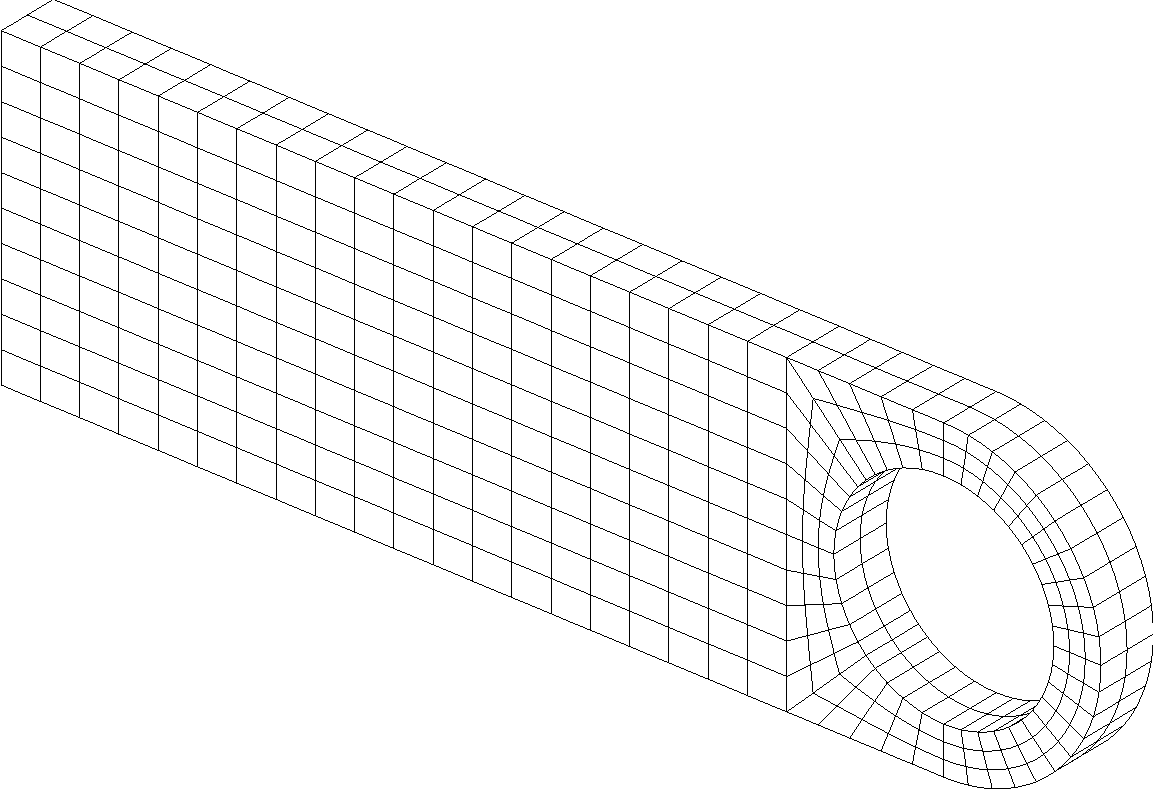
\includegraphics[height=0.242\textheight]{images/exo/1.2_maillage_hexa.4} \hspace{2mm}
          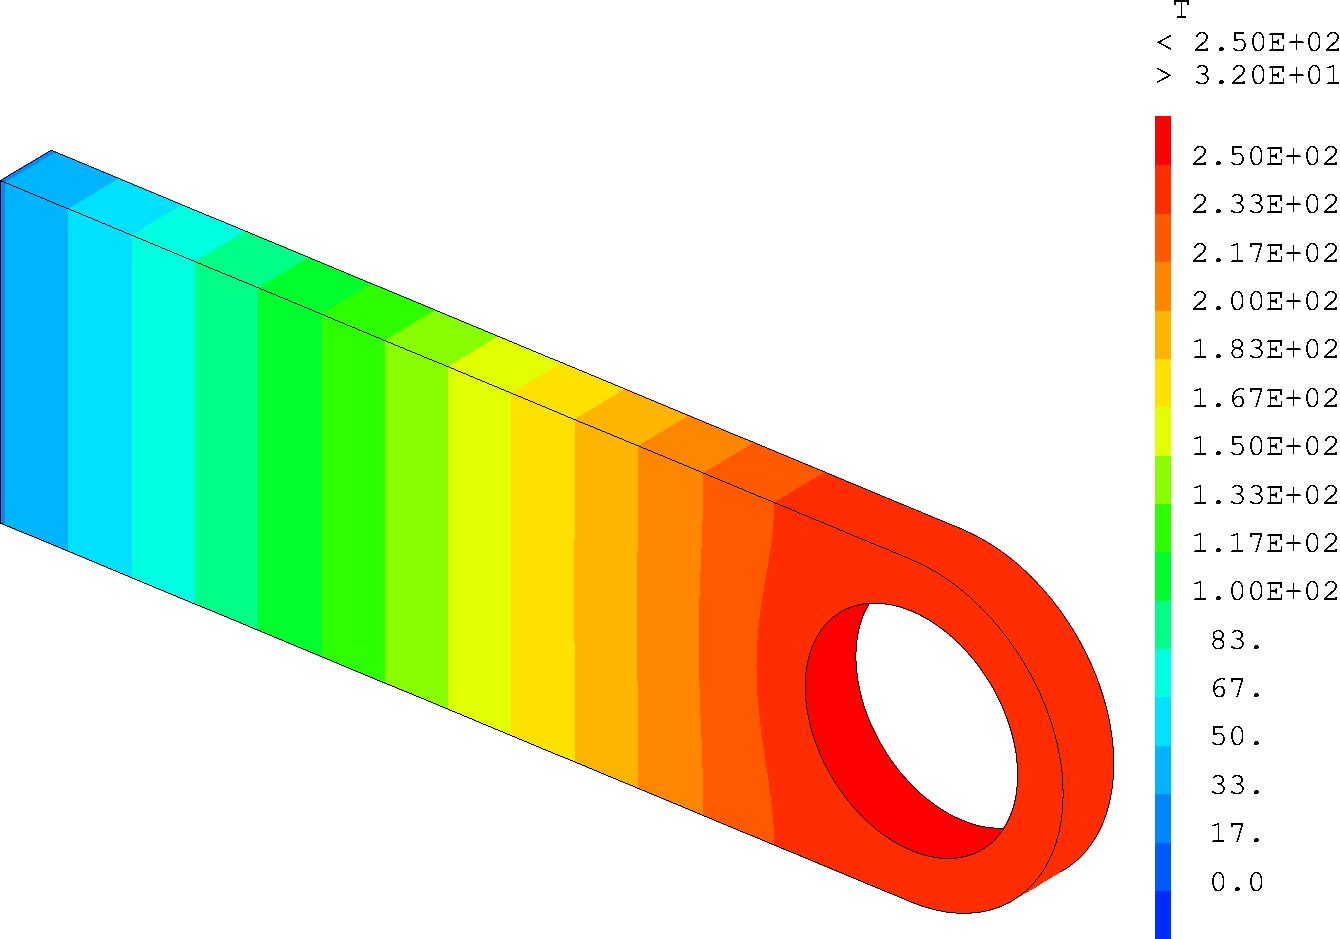
\includegraphics[height=0.275\textheight]{images/exo/2.1_temperatures.3}  \hspace{2mm}
          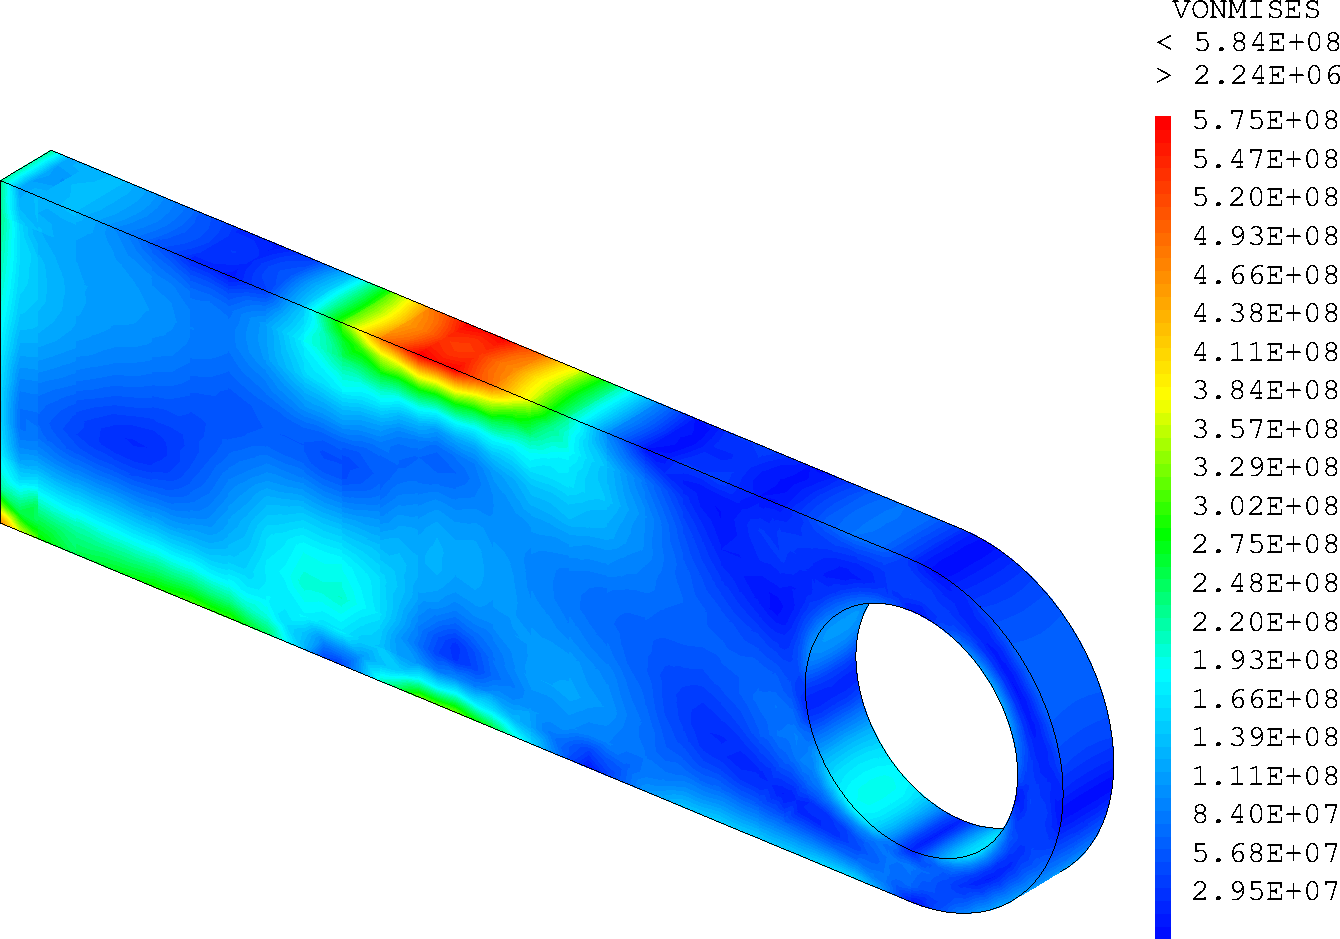
\includegraphics[height=0.275\textheight]{images/exo/8_contraintes}
          \end{center}
    \item \fe{\hyperlink{complements}{Compléments}}
             {\hyperlink{complements}{Complements}}
  \end{itemize}
\end{frame}

%%%%%%%%%%%%%%%%%%%%%%%%%%%%%%%%%%%%%%%%%%%%%%%%%%%
\fe{\section{Présentation}}{\section{Presentation}}
\label{presentation}
%%%%%%%%%%%%%%%%%%%%%%%%%%%%%%%%%%%%%%%%%%%%%%%%%%%

\begin{frame}{\fe{Cast3M, quid ?}{What is Cast3M?}}
  \begin{center}
    \fe{Logiciel de simulation utilisant la \g{méthode des éléments finis} en \g{mécanique/thermique} des \g{structures} et des \g{fluides}}
       {A simulation software using the \g{finite element method} in \g{thermal and mechanical} analysis of \g{structures} and \g{fluids}}\pause
  \end{center}
  \begin{itemize}
    \item \fe{Résolution d'\g{équations aux dérivées partielles}}
             {\g{Partial differential equations} solver}\pause
    \item \fe{\g{Système complet} : solveur, pré/post-processeur, visualisation, import/export des données\dots}
             {\g{Complete software}: solver, pre-processing and post-processing, visualization, reading/writing data\dots}\\~\\
    \begin{center}
      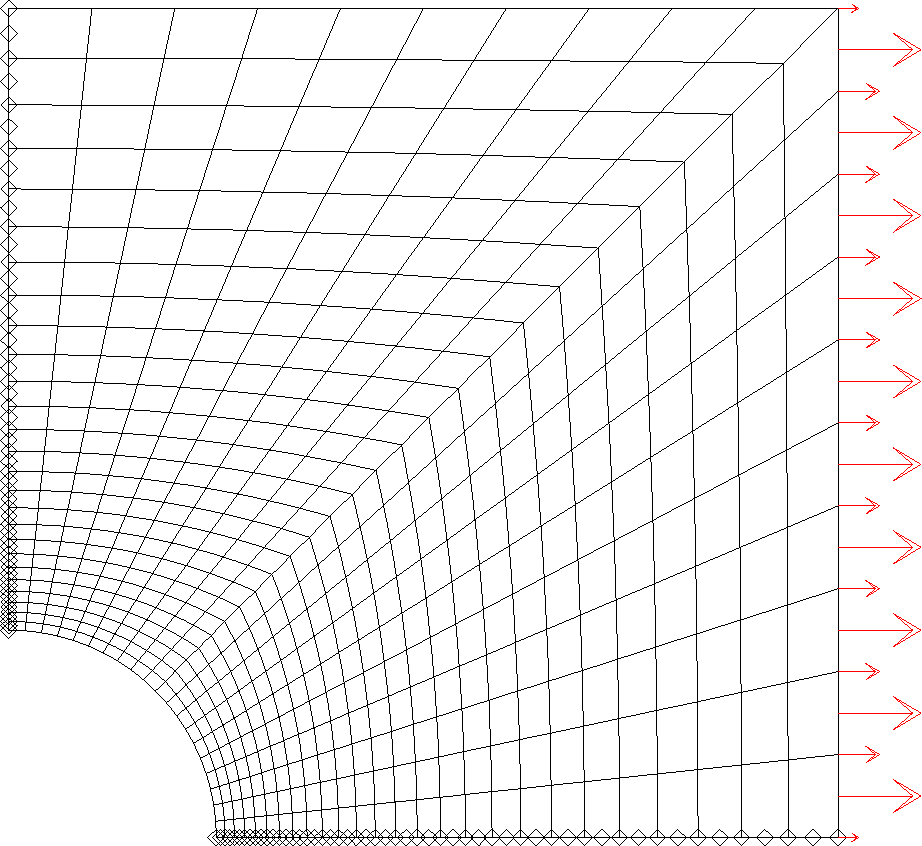
\includegraphics[height=0.25\textheight]{images/plaque.1} \:
      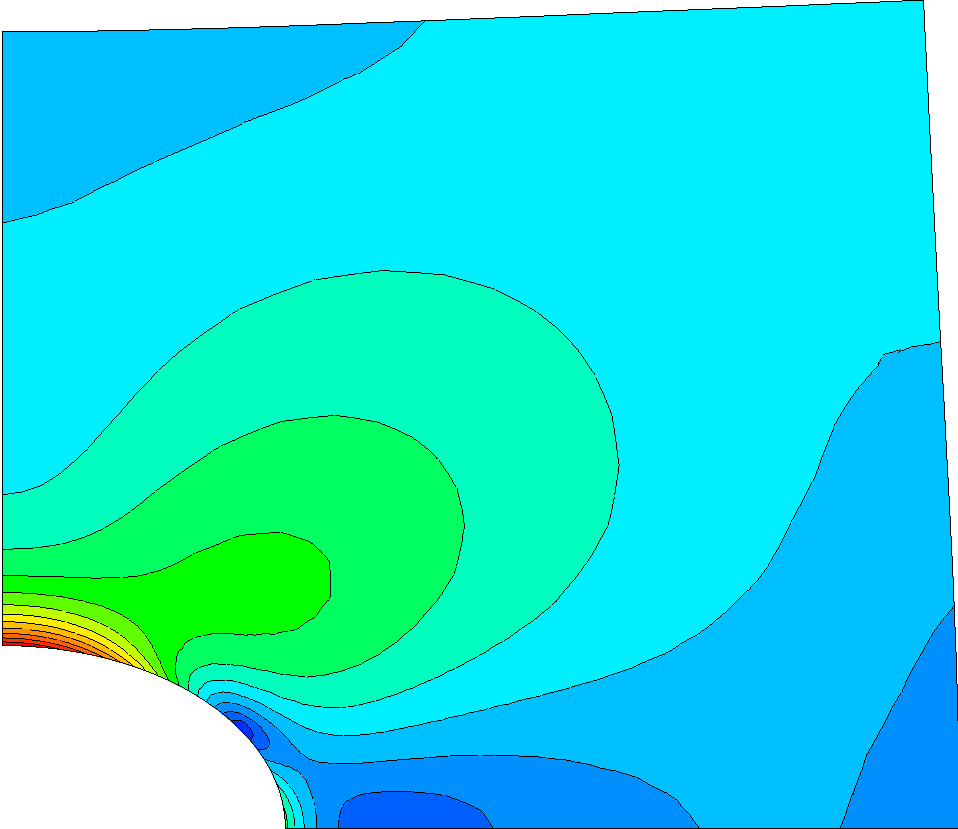
\includegraphics[height=0.25\textheight]{images/plaque.2} \:
      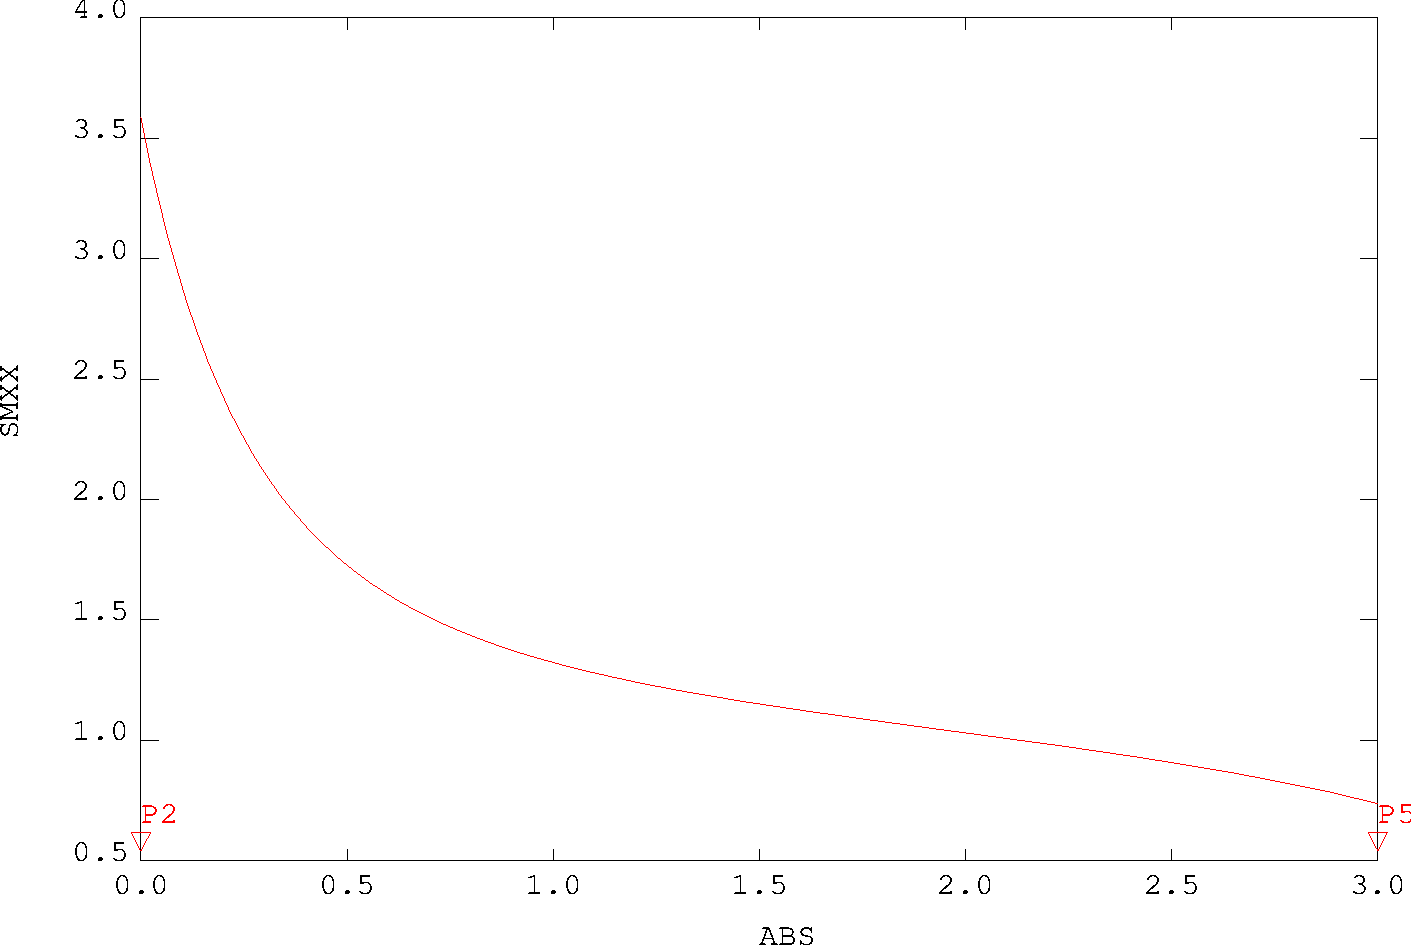
\includegraphics[height=0.25\textheight]{images/plaque.3}
    \end{center}\pause
    \item \fe{Basé sur un langage de commande : \g{Gibiane} (orienté objet)}
             {Based on a programming language: \g{Gibiane} (objet-oriented)}\\
  \end{itemize}
\end{frame}

\begin{frame}{\fe{Nombreux domaines d'application}{Wide range of applications}}
  \small
  \begin{itemize}
    \item<1->\fe{\g{Mécanique des structures}}{\g{Structural mechanics}}\\
    \footnotesize
    \fe{\red{Quasi-statique} (non linéarités matériau, géométrie, conditions limites)}
       {\red{Quasi-static} (non linear behavior, geometry, boundary conditions)}\\
    \onslide<1>{
      \begin{textblock*}{4cm}(0cm,0cm)
        \begin{center}
          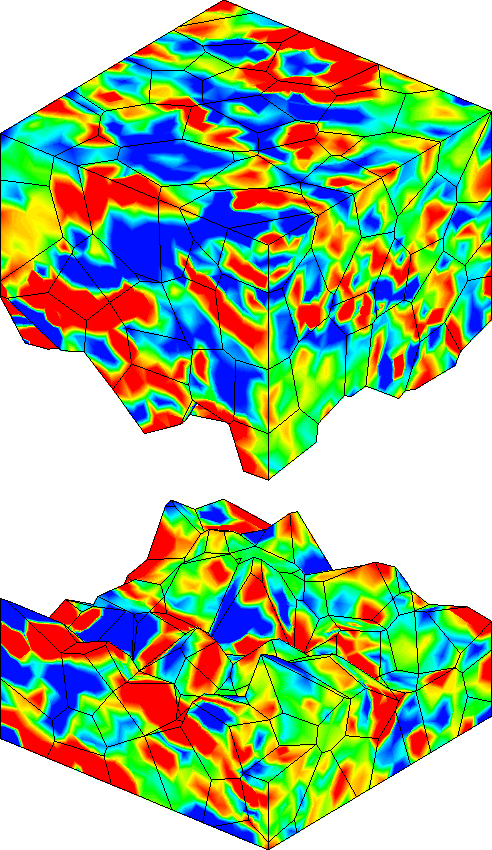
\includegraphics[height=0.4\textheight]{images/polycristal}\\
          \tiny{\fe{\emph{Microstructure : agrégat polycristallin}}{\emph{Microstructure: polycrystalline aggregate}}}
        \end{center}
      \end{textblock*}
      \begin{textblock*}{4cm}(3.4cm,0.8cm)
        \begin{center}
          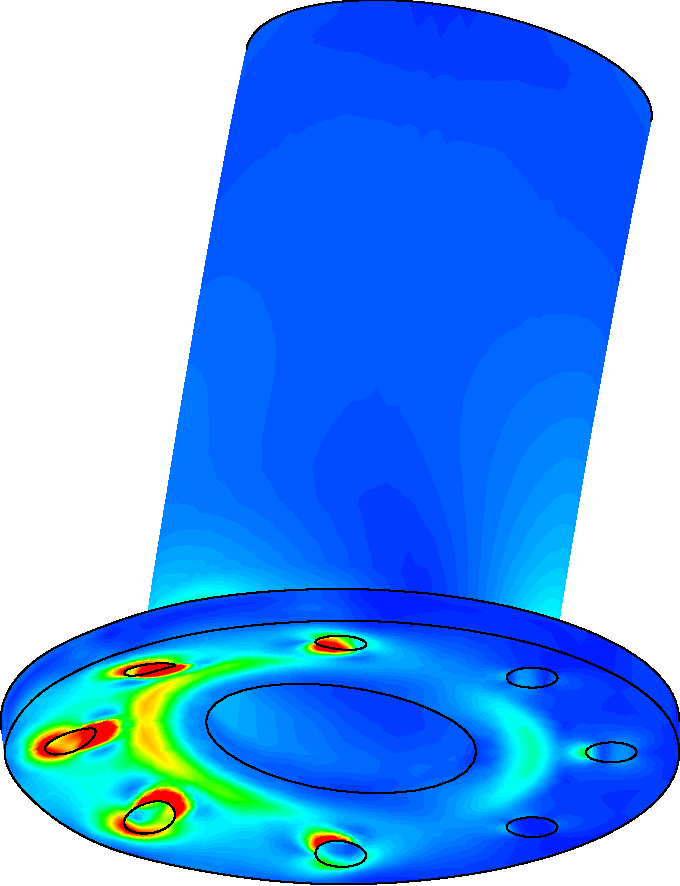
\includegraphics[height=0.4\textheight]{images/tube}\\
          \tiny{\fe{\emph{Composant : liaison d'un tube}}{\emph{Component: connection on a tube}}}
        \end{center}
      \end{textblock*}
      \begin{textblock*}{5cm}(7.2cm,1.6cm)
        \begin{center}
          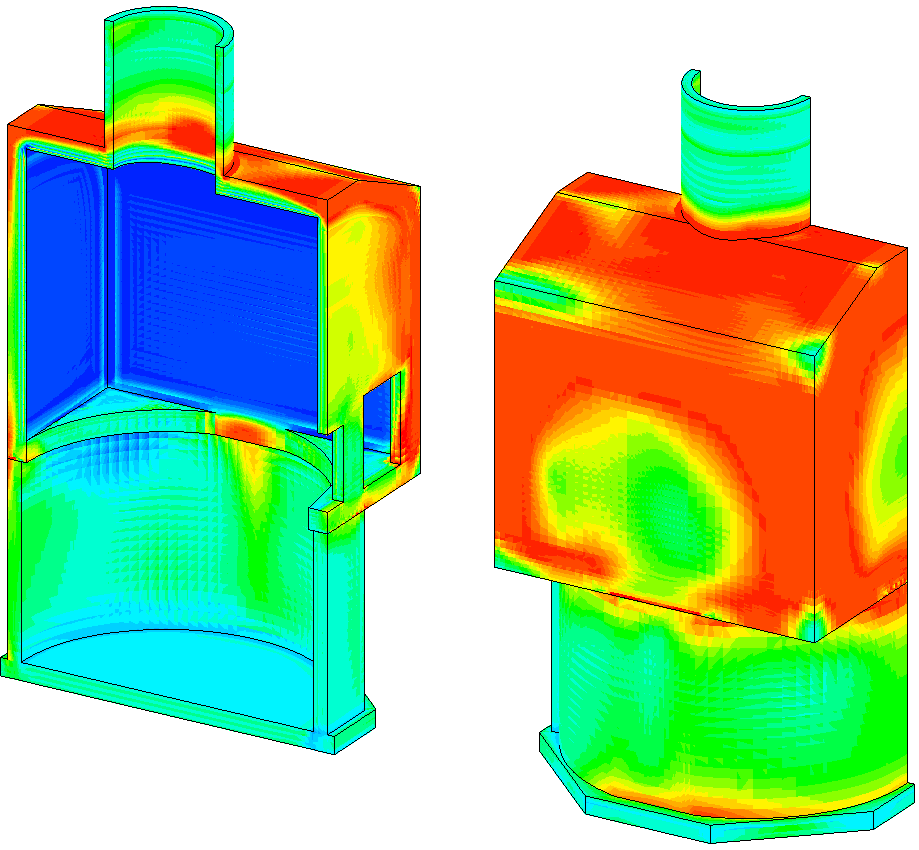
\includegraphics[height=0.4\textheight]{images/galatee}\\
          \tiny{\fe{\emph{Batiment en béton armé (S. Durand)}}{\emph{Reinforced concrete building (S. Durand)}}}
        \end{center}
      \end{textblock*}
      }
    \onslide<2->\fe{\orange{Contact/frottement}, \green{Flambage}}
                    {\orange{Contact/friction}, \green{Buckling}}\\
    \onslide<2>{
      \begin{textblock*}{10cm}(1cm,0.2cm)
        \begin{center}
          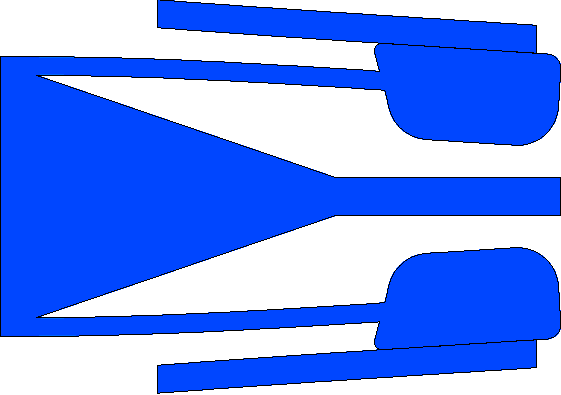
\includegraphics[height=0.25\textheight]{images/sac_a_dos.15}
          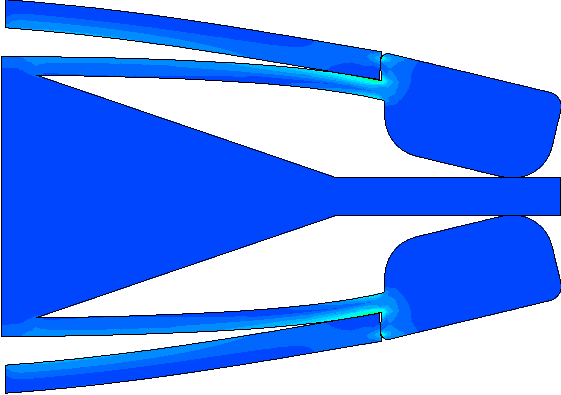
\includegraphics[height=0.25\textheight]{images/sac_a_dos.32}
          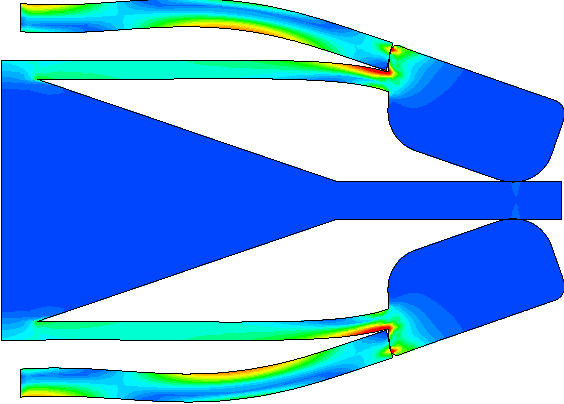
\includegraphics[height=0.25\textheight]{images/sac_a_dos.41}\\
          \tiny{\fe{\emph{Attachement d'un clip (contact + plasticité)}}{\emph{Locking a clip buckle (contact + plasticity)}}}
        \end{center}
      \end{textblock*}
      }
    \onslide<3->\fe{\blue{Dynamique} (temporelle, modale, interaction fluide structure)}
                   {\blue{Dynamic} (temporal, modal, fluid structure interaction)}\\
    \onslide<3>{
      \begin{textblock*}{10cm}(1cm,0.2cm)
        \begin{center}
          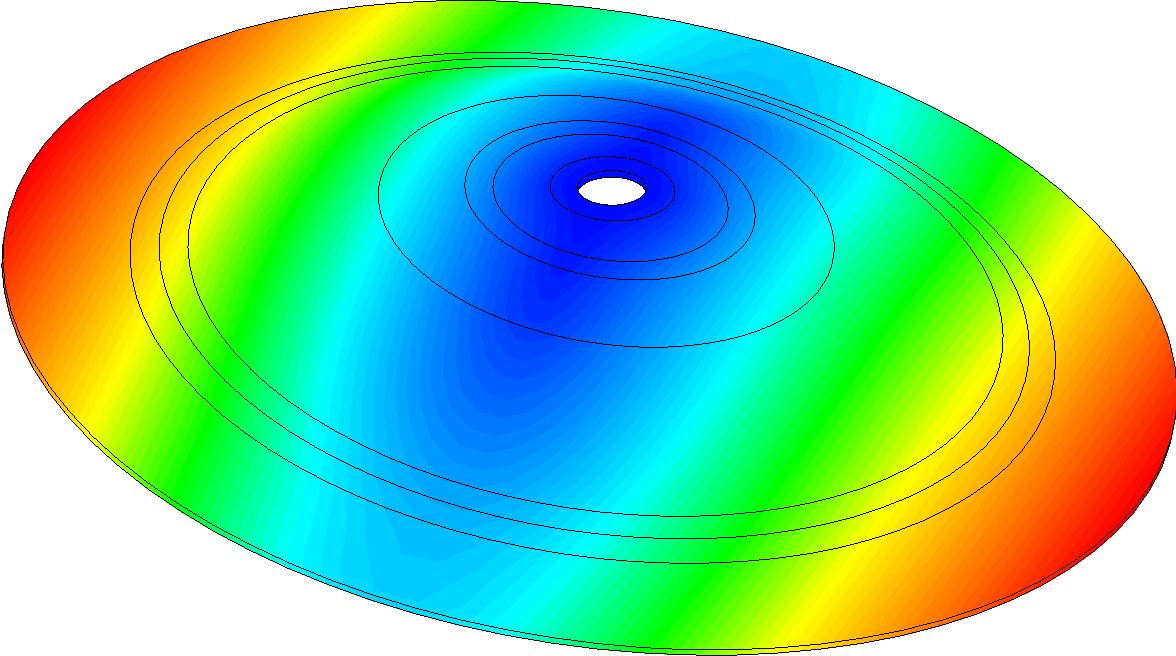
\includegraphics[height=0.2\textheight]{images/cymbale_mode_1}
          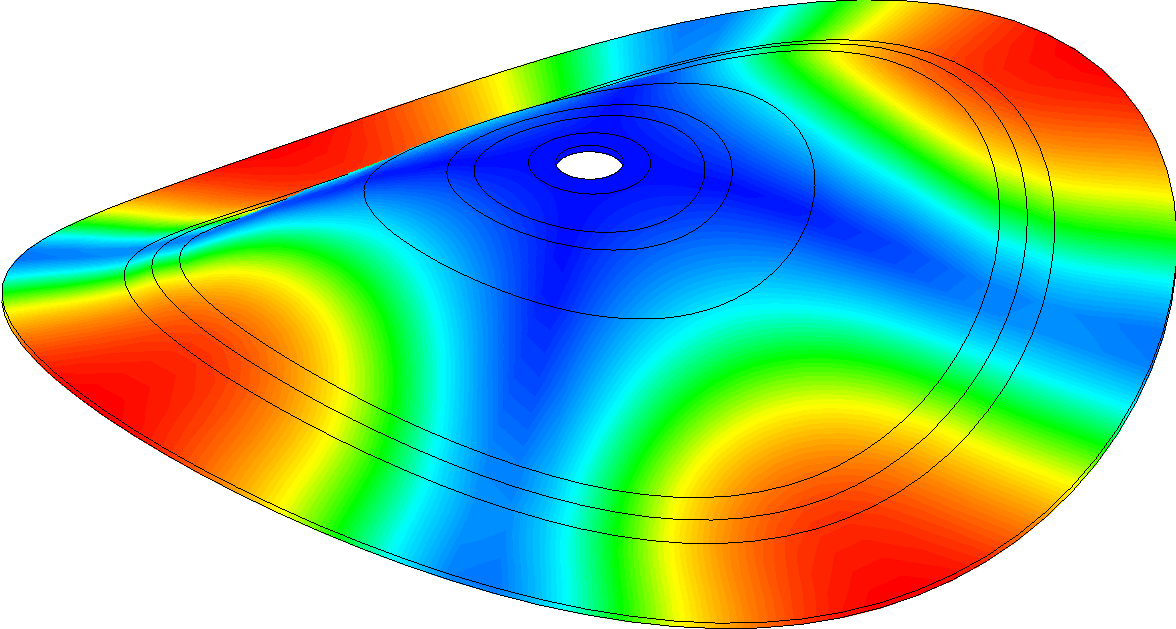
\includegraphics[height=0.2\textheight]{images/cymbale_mode_2}
          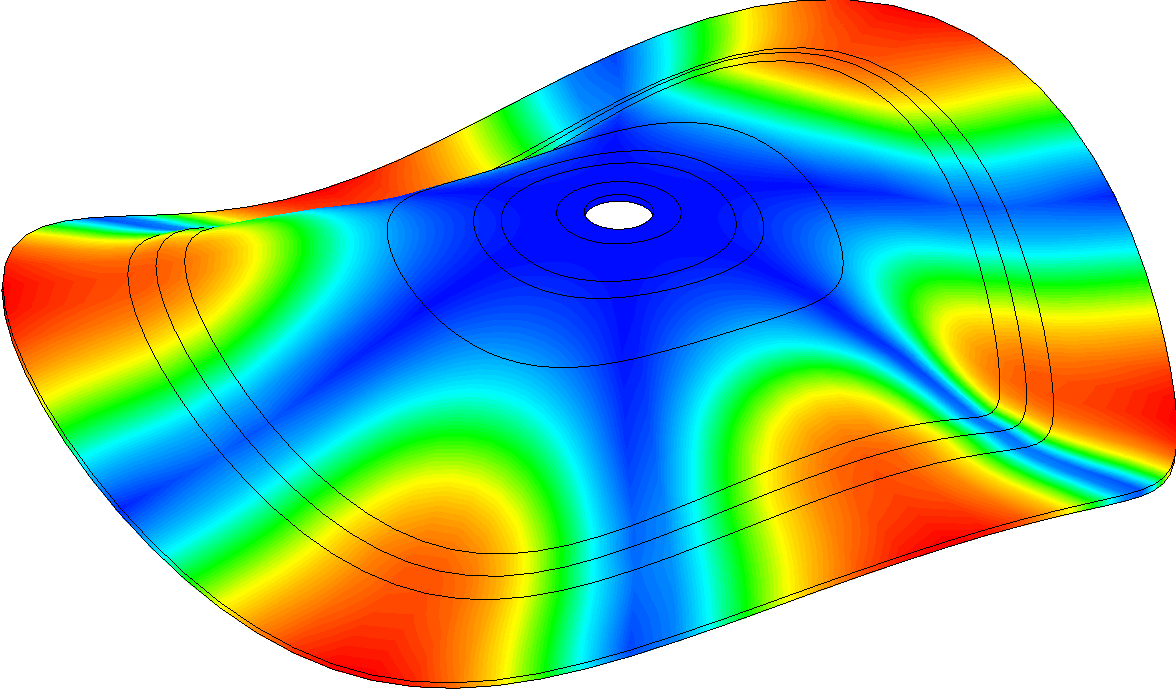
\includegraphics[height=0.2\textheight]{images/cymbale_mode_4}\\
          \tiny{\fe{\emph{Premiers modes propres d'une cymbale}}{\emph{First eigenmodes of a cymbal}}}
        \end{center}
      \end{textblock*}
      }
    \onslide<4->{\fe{\violet{Rupture} (XFEM, propagation dynamique, zones cohésives)}
                    {\violet{Fracture} (XFEM, dynamic propagation, cohesive zones models)}}\\
    \only<4>{
      \begin{textblock*}{11cm}(1cm,0cm)
        \begin{center}
          \if \animation 1
            \animategraphics[controls,loop,poster=last,height=4cm]{3}{images/rupture_ct/rupture_ct_}{1}{8}
            \animategraphics[controls,loop,poster=last,height=4cm]{3}{images/rupture_ct/rupture_ct_detail_}{1}{8}\\
          \else
            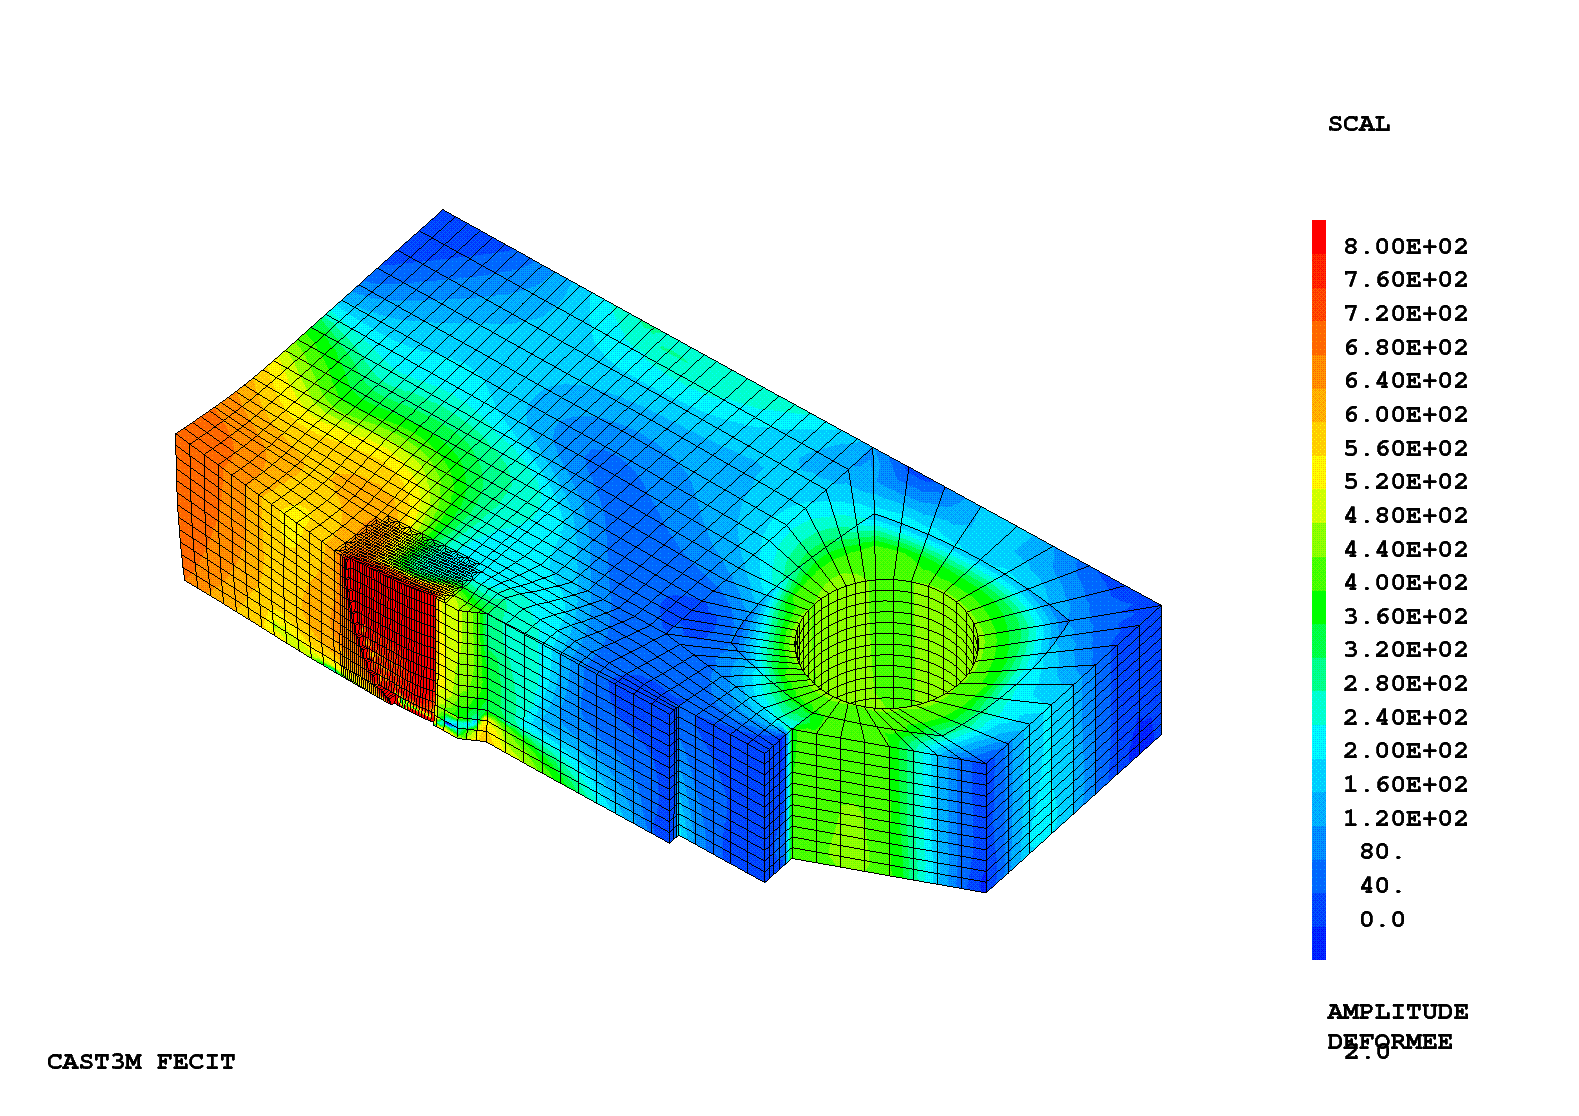
\includegraphics[height=4cm]{images/rupture_ct/rupture_ct_8}
            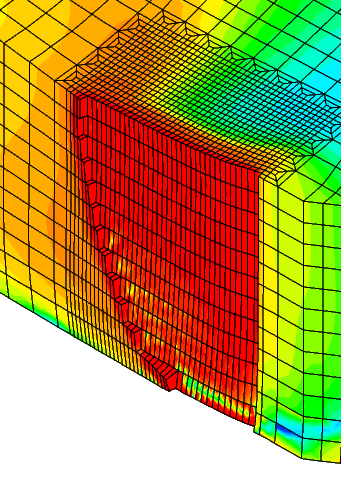
\includegraphics[height=4cm]{images/rupture_ct/rupture_ct_detail_8}\\
          \fi
          \tiny{\fe{\emph{Rupture d'éprouvette CT, plasticité/endommagement, suppression d'éléments lors du calcul (S. Kebiri)}}
                   {\emph{Fracture of a CT sepcimen, plasticity/dammage, elements removal during computation (S. Kebiri)}}}
        \end{center}
      \end{textblock*}
      }
    \small
    \item<5->\fe{\g{Thermique}}{\g{Thermal analysis}}\\
    \footnotesize
    \onslide<5->{\fe{Conduction, convection, rayonnement, changement de phase}
                    {Conduction, convection, radiation, phase transition}}\\
    \onslide<5>{
      \begin{textblock*}{10cm}(1cm,0.1cm)
        \begin{center}
          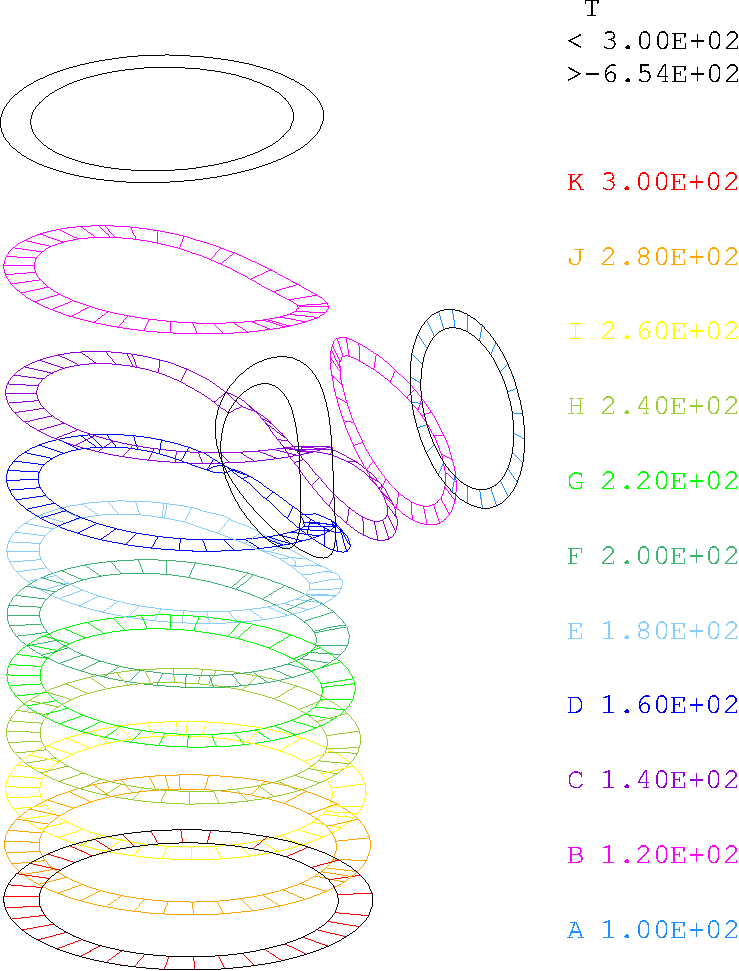
\includegraphics[height=0.4\textheight]{images/te_temperature}\hspace{1cm}
          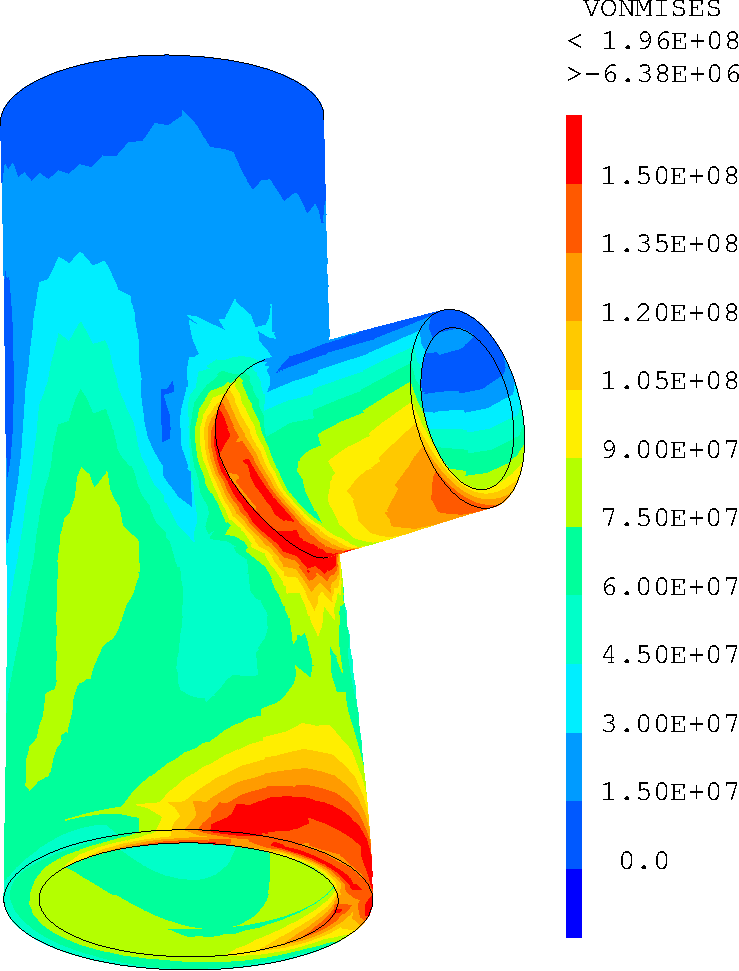
\includegraphics[height=0.4\textheight]{images/te_sigma}\\
          \tiny{\fe{\emph{Thermo mécanique d'un té de tuyauterie}}{\emph{Thermo mechanical analysis of a pipe tee}}}
        \end{center}
      \end{textblock*}
      }
    \small
    \item<6-> \fe{\g{Mécanique des fluides}}{\g{Fluid mechanics}}
    \item<6-> \fe{\g{Diffusion} multi espèces (loi de Fick)}{Multi species \g{diffusion} (Fick's law)}\\
    \item<6-> \fe{Fabrication additive, Métallurgie}{Additive manufacturing, Metallurgy}\\
    \footnotesize
    \only<6>{
      \begin{textblock*}{7cm}(5.7cm,-2cm)
        \begin{center}
          \if \animation 1
            \animategraphics[controls,loop,poster=last,width=5cm]{20}{images/fab_add/fab_add_}{001}{397}\\
          \else
            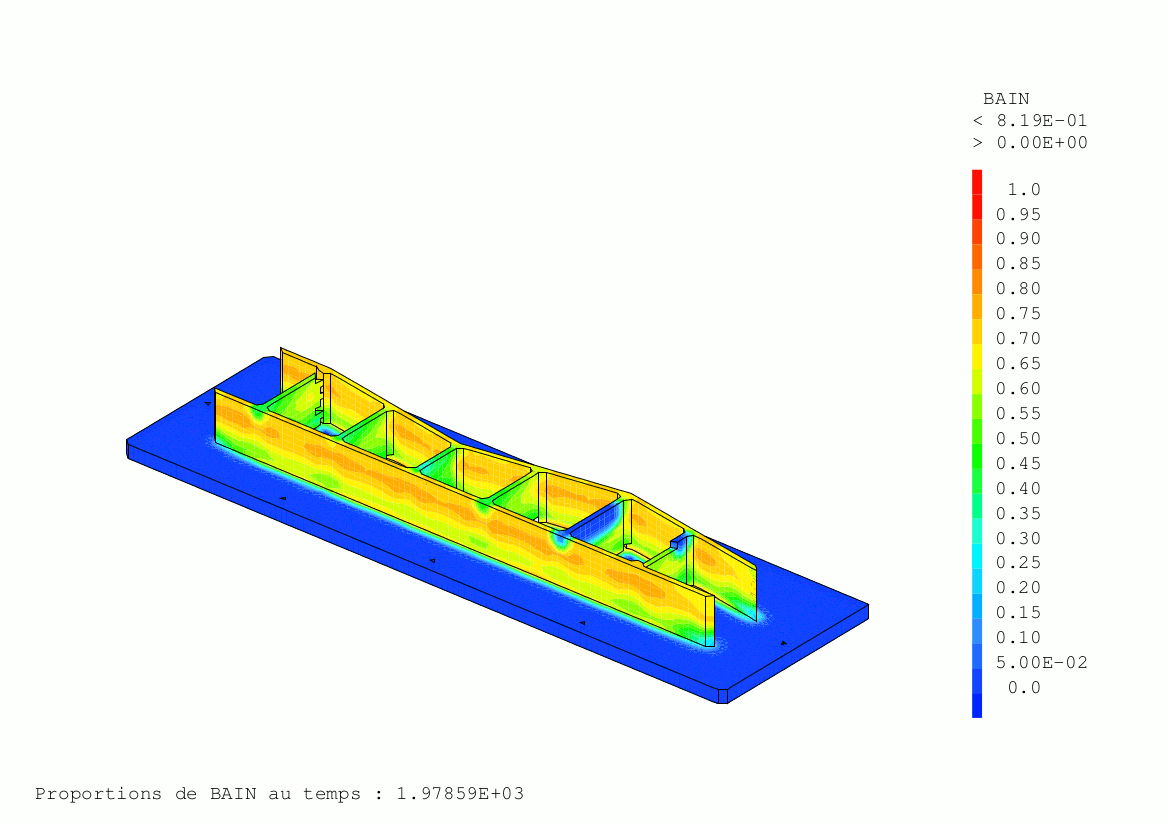
\includegraphics[width=5cm]{images/fab_add/fab_add_397}\\
          \fi
          \tiny{\fe{\emph{Proportion de bainite lors d'une fabrication additive (C. Berthinier)}}
                   {\emph{Proportion of bainite during the additive manufacturing (C. Berthinier)}}}
        \end{center}
      \end{textblock*}
      }
    \onslide<7>{
      \begin{textblock*}{5cm}(6.5cm,-1.5cm)
        \begin{center}
          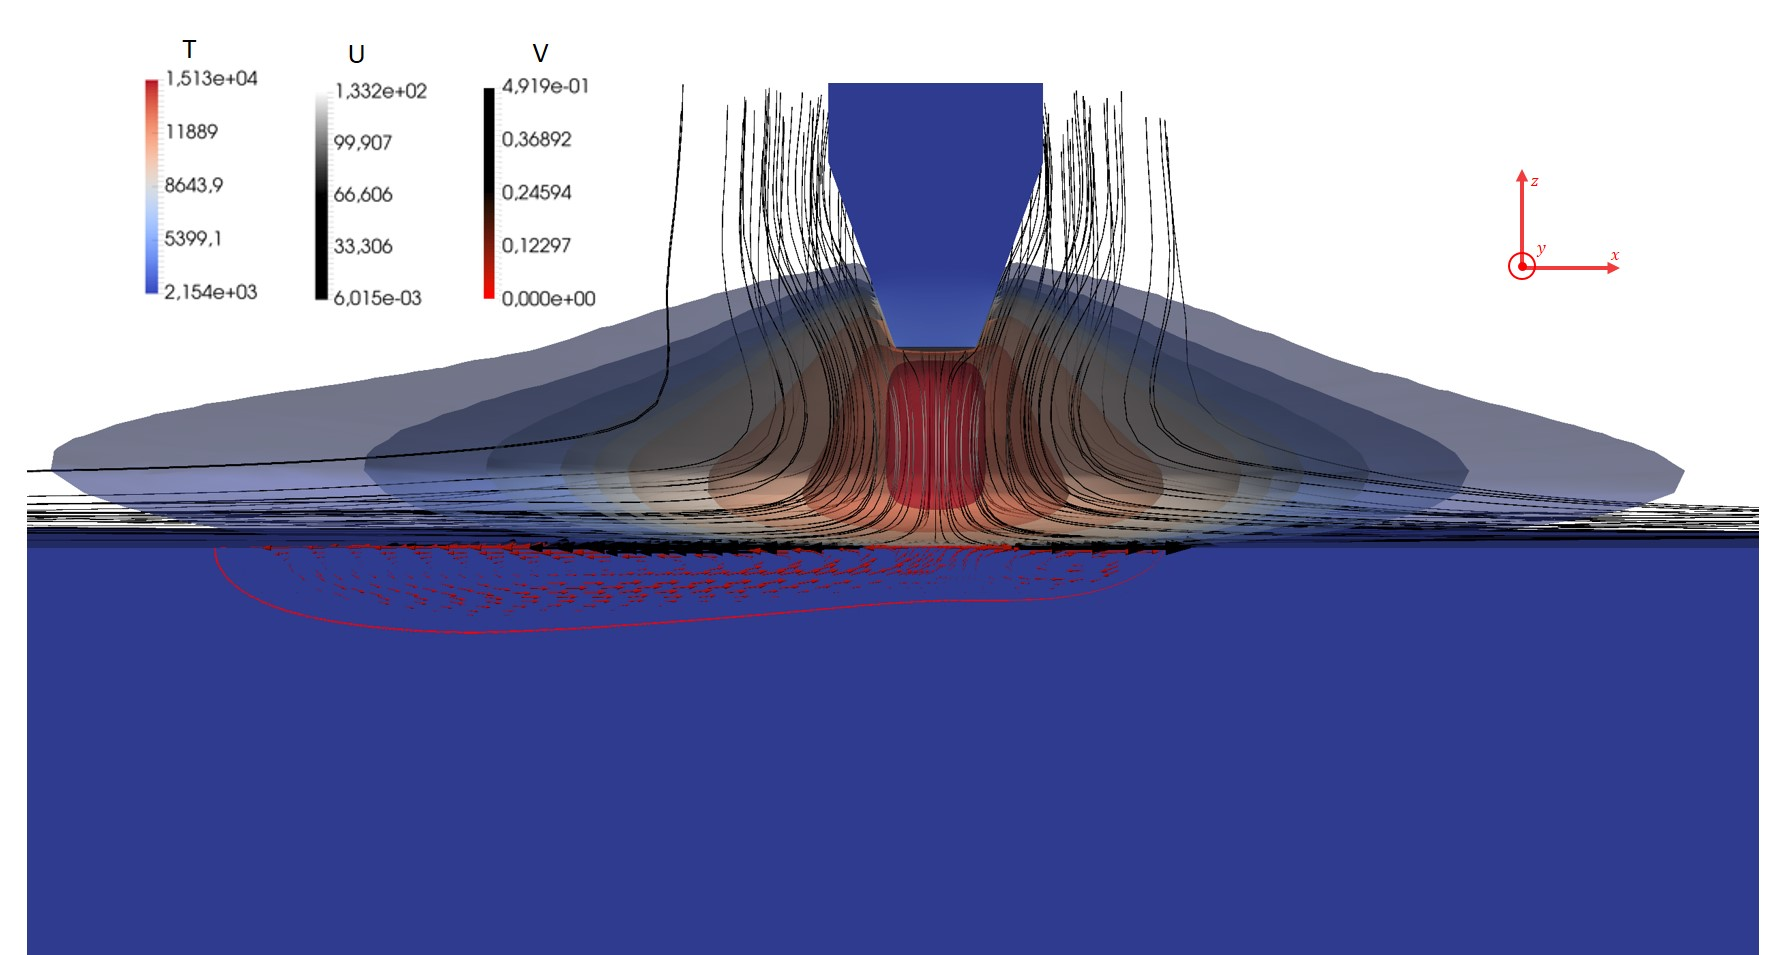
\includegraphics[width=5cm]{images/soudage}\\
          \tiny{\fe{\emph{Simulation magnéto thermo hydrodynamique du soudage TIG (arc plasma + bain) (C. Nahed)}}
                   {\emph{Magneto thermo hydro dynamic simulation of TIG welding (plasma arc + weld pool) (C. Nahed)}}}
        \end{center}
      \end{textblock*}
      }
    \small
    \item<8-> \fe{Magnétostatique}{Magneto-statics}
    \item<8-> \fe{Couplage thermo-hygro-mécanique}{Thermo-hygro-mechanics coupling}
    \item<8-> \fe{Optimisation topologique}{Topology optimization}
    \only<8>{
      \begin{textblock*}{5cm}(6.2cm,-6cm)
        \begin{center}
          \if \animation 1
            \animategraphics[controls,loop,poster=last,width=6cm]{10}{images/topoptim/topoptim.}{001}{100}\\~\\
          \else
            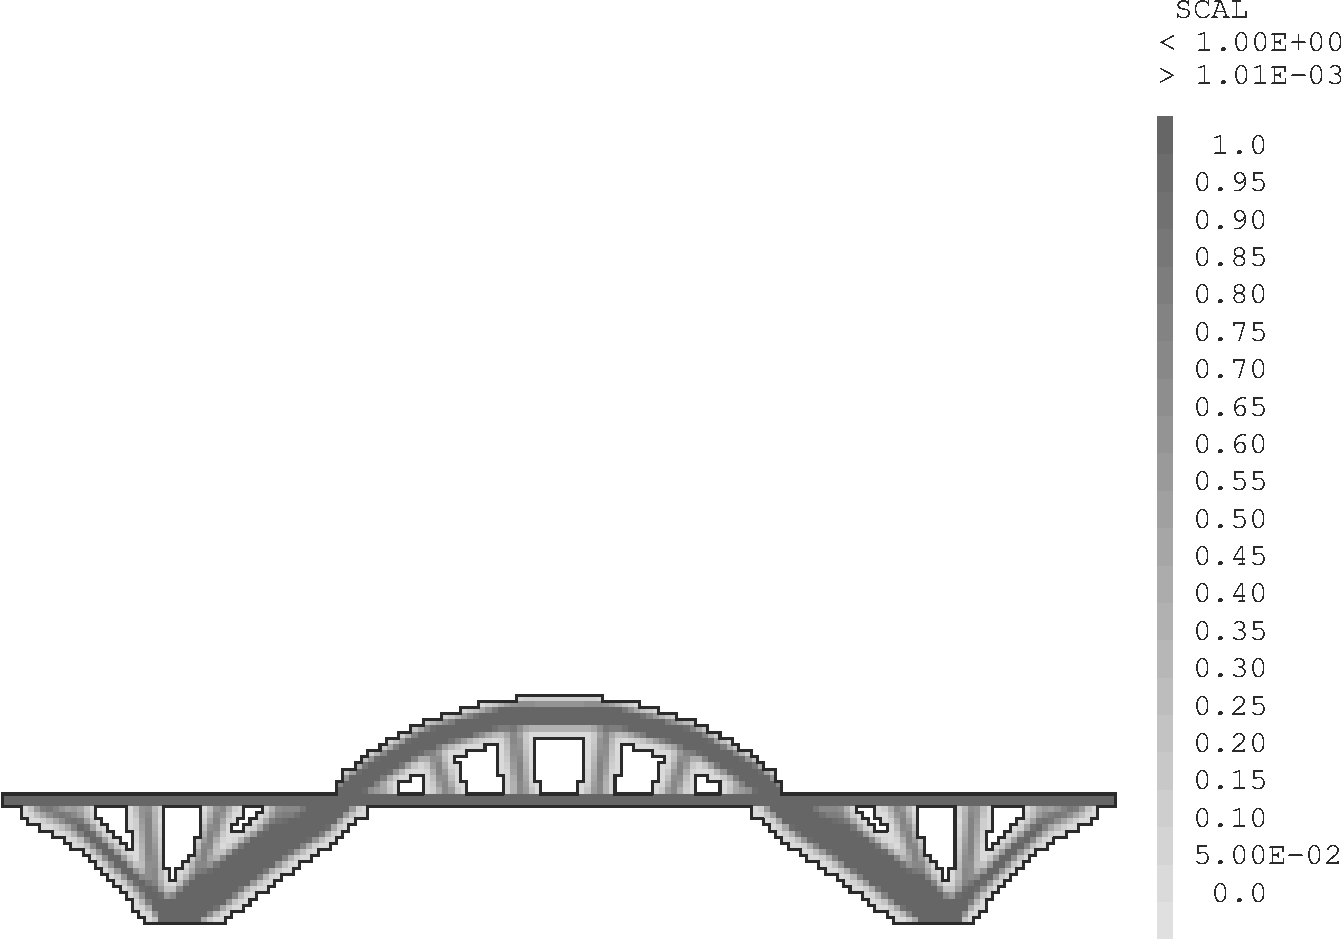
\includegraphics[width=6cm]{images/topoptim/topoptim.100}\\~\\
          \fi
          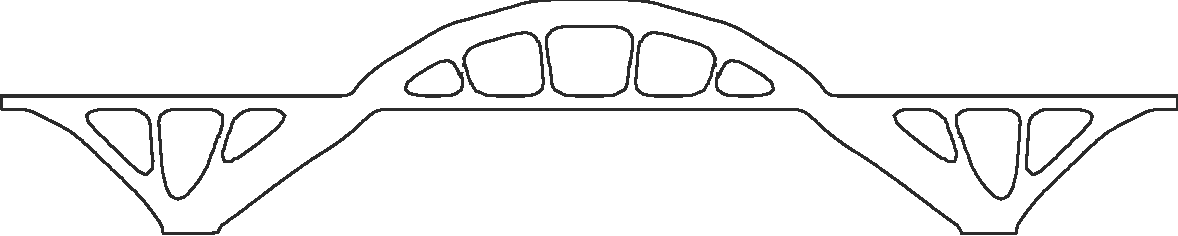
\includegraphics[width=5cm]{images/topoptim/toposurf}\\
          \tiny{\fe{\emph{Optimisation topologique d'un pont}}{\emph{Topology optimization of a bridge}}}
        \end{center}
      \end{textblock*}
      }
  \end{itemize}
\end{frame}

\begin{frame}{\fe{Comment obtenir Cast3M ?}{How to get Cast3M}}
  \begin{itemize}
    \item \fe{Multi plateformes}{Cross platform}\\
    \footnotesize
    \blue{Windows}, \red{Linux}, \green{macOS}
    \normalsize
    \item \fe{Où télécharger Cast3M ?}{Where can I download Cast3M?}\\
    \footnotesize
    \url{http://www-cast3m.cea.fr/index.php?page=dlcastem}
    \normalsize
    \item \fe{Accès au code source}{Access to the source code}\\
    \footnotesize
    \fe{Développement communautaire}{Open collaboration}\\
    \fe{Compilateur / éditeur de liens fournis}{Compiler / Linker are provided}
    \normalsize
    \item \fe{Prix}{Price}\\
    \footnotesize
    \fe{\green{Gratuit} pour la recherche et l'enseignement\\
        \red{Payant} pour une utilisation commerciale}
       {\green{Free} license, for education and research use\\
        \red{Paid} license, for enterprise use}
    \normalsize
    \item \fe{Utilisateurs/clients}{Users/customers}\\
    \footnotesize
    \fe{Universités, écoles d'ingénieurs\\
        IRSN, EDF, SNCF, CNRS, Framatome, Air Liquide, CERN, \dots}
       {Universities, engineering schools\\
        IRSN, EDF, SNCF, CNRS, Framatome, Air Liquide, CERN, \dots}\\
    \scriptsize
    \fe{Outil de référence IRSN pour les analyse de sureté des installations nucléaires françaises\\
        Outil de référence Framatome pour l'analyse en mécanique de la rupture}
       {Reference FEM tool for IRSN for safety analysis of French nuclear installations\\
        Reference tool for Framatome for fracture mechanics}
    \normalsize
    \end{itemize}
\end{frame}

\begin{frame}{\fe{Comment utiliser Cast3M ?}{How to launch Cast3M?}}
  \begin{textblock*}{5cm}(7.9cm,0cm)
    \if \animation 1
      \animategraphics[autoplay,loop,poster=last,width=4.5cm]{10}{images/new_dgibi/new_dgibi-}{000}{235}
    \else
      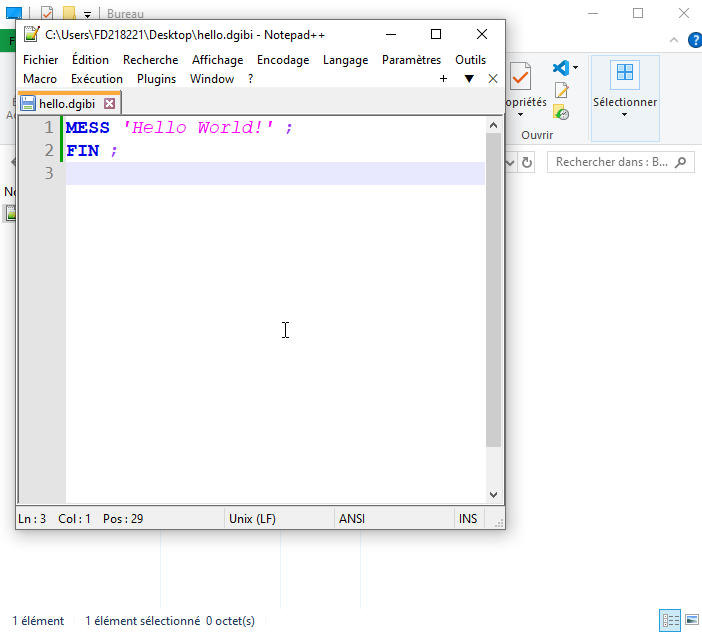
\includegraphics[width=4.5cm]{images/new_dgibi/new_dgibi-235}
    \fi
  \end{textblock*}
  \begin{enumerate}
    \item\fe{Écrire un fichier texte en Gibiane}{Write a Gibiane script in a text file}\\
    \footnotesize
    \fe{et l'enregistrer dans un répertoire de travail}{and save it in a working directory}
    \normalsize
    \item[]\white{O/}\\
    \footnotesize
    \white{et}\\
    \normalsize
    \item[]\white{Cast3M}\\
    \footnotesize
    \white{castem24  hello.dgibi}
    \normalsize
    \item[]\white{U}\\
    \footnotesize
    \white{mode}\\
    \white{castem24}
    \normalsize
  \end{enumerate}
\end{frame}

\begin{frame}{\fe{Comment utiliser Cast3M ?}{How to launch Cast3M?}}
  \begin{textblock*}{5cm}(7.9cm,0cm)
    \if \animation 1
      \animategraphics[autoplay,loop,poster=last,width=4.5cm]{10}{images/new_cmd/new_cmd-}{000}{179}
    \else
      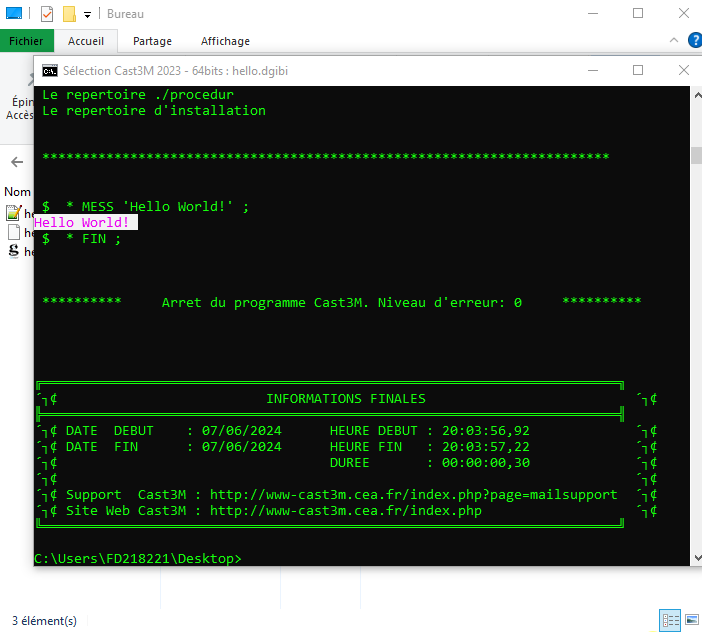
\includegraphics[width=4.5cm]{images/new_cmd/new_cmd-179}
    \fi
  \end{textblock*}
  \begin{enumerate}
    \item\fe{Écrire un fichier texte en Gibiane}{Write a Gibiane script in a text file}\\
    \footnotesize
    \fe{et l'enregistrer dans un répertoire de travail}{and save it in a working directory}
    \normalsize
    \item\fe{Ouvrir un terminal / invite de commandes}{Open a terminal / command prompt}\\
    \footnotesize
    \fe{et se placer dans le répertoire}{and go to the working directory}\\
    \normalsize
    \item\fe{Lancer Cast3M sur ce fichier}{Launch Cast3M on this file}\\
    \footnotesize
    \kwr{castem24 }\kw{ hello.dgibi}
    \normalsize
    \item\fe{Utilisable aussi sans fichier}{Can also be use without file}\\
    \footnotesize
    \fe{mode interactif}{interactive mode}\\
    \kwr{castem24}
    \normalsize
  \end{enumerate}
\end{frame}

\begin{frame}{\fe{Le site web Cast3M}{The Cast3M web site}}
  \begin{center}
    \url{http://www-cast3m.cea.fr/}
  \end{center}
  \begin{itemize}
    \item \fe{Présentation de Cast3M}{Cast3M presentation}
    \item \fe{Formation et tutoriels vidéo}{Training courses and video tutorials}
    \item \fe{Documentation (notices, manuels, sources, exemples)}{Documentation (manual pages, source code, examples)}
    \item \fe{Fiches d'anomalie et de développement}{Anomaly and development reports}
    \item \fe{Téléchargements}{Downloads}
    \item \fe{Contact : support Cast3M}{Contact: Cast3M support}
    \item \fe{Communauté : liste de diffusion, club Cast3M}{Community: mailing list, Cast3M club}
  \end{itemize}
\end{frame}

%%%%%%%%%%%%%%%%%%%%%%%%%%%%%%%%%%%%%%%%%%%%%%%%%%%%%%%%%%
\fe{\section{Langage Gibiane}}{\section{Gibiane Language}}
\label{gibiane}
%%%%%%%%%%%%%%%%%%%%%%%%%%%%%%%%%%%%%%%%%%%%%%%%%%%%%%%%%%

\begin{frame}{\fe{Le langage Gibiane}{The Gibiane language}}
  \begin{itemize}
    \item \fe{\red{Langage de programmation} destiné au calcul EF}
             {\red{Programming language} dedicated to FE calculation}\\
    \footnotesize
    \begin{textblock*}{5cm}(7cm,0.5cm)
      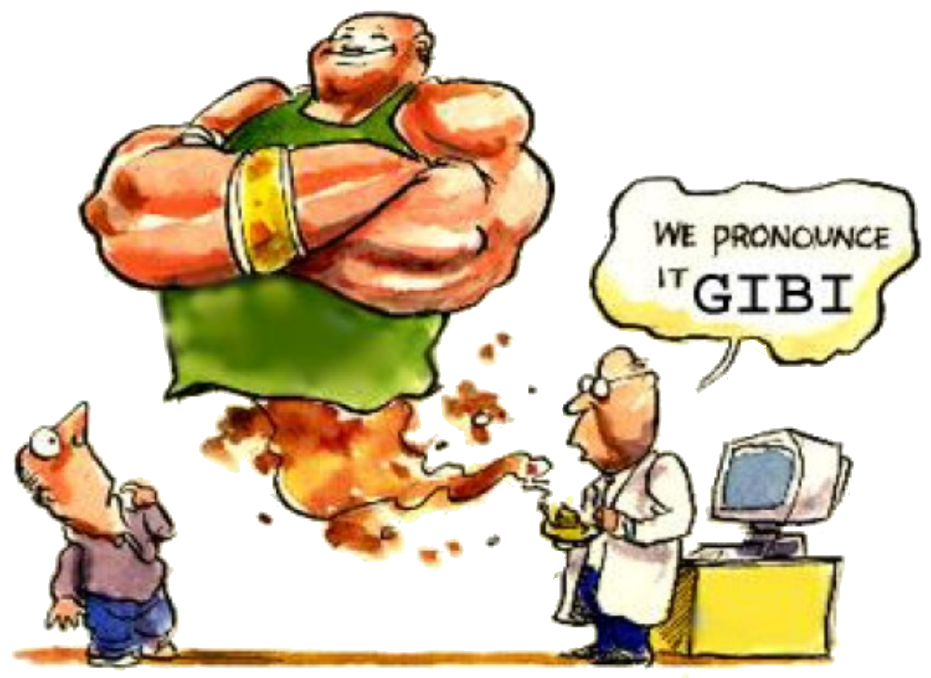
\includegraphics[width=3cm]{images/gibi_genie}
    \end{textblock*}
    \fe{Objets classiques (entiers, flottants, chaines, logiques, tables)\\
        Instructions conditionnelles\\
        Boucles itératives\\
        Sous structuration\\
        Récursivité}
       {Classical objects (integer, floating-point, string, logical , tables)\\
       Flow control statements\\
       Loops and iterations\\
       Subroutines\\
       Recursion}
    \normalsize
    \item \fe{Langage \red{interprété}}{\red{Interpreted} language}\\
    \footnotesize
    \fe{Le programme peut être exécuté dès que le script est modifié\\
        Le programme peut être exécuté en mode interactif}
       {You can run the program as soon as you make changes to the file\\
       You can run it in a interactive mode}
    \normalsize
    \item \fe{Langage \red{orienté objet}}{\red{Object-oriented} language}\\
    \footnotesize
    \fe{Tout est traité comme un objet\\
        Pas besoin de déclarer les variables ou de spécifier leur type}
       {Everything in the program is treated as an object\\
       No need to declare variables or to specify the type of a variable}
    \normalsize
    \item \fe{Mots clefs en français}{French key words}
    \item \fe{Programmation facile et rapide}{Easy to learn, easy to read}
  \end{itemize}
\end{frame}

\begin{frame}{\fe{Gibiane : règles de syntaxe}{Gibiane: syntax rules}}
  \begin{itemize}
    \item \fe{Ligne(s) de commande}{Statements lines}\\
    \footnotesize
    \fe{\red{500 caractères max} par instruction\\
        Une instruction peut être écrite sur plusieurs lignes\\
        Se \red{termine par un point virgule \kw{;}}\\
        Le \red{symbole d'affectation} est le signe égal \kwr{=}}
       {\red{500 characters max} per statement\\
        A statement can be written on several lines\\
        \red{End with a semicolon \kw{;}}\\
        The \red{assignment operator} is the equals sign \kwr{=}}
    \normalsize
    \item \fe{Insensibilité à la casse}{Case insensitive}\\
    \footnotesize
    \kw{TOTO = 3.14 ;}\\
    \kw{A~~~ = 2.~}\kwr{*}\kw{~tOTo ;}
    \fe{la variable \kw{A} vaut bien 6.28}{variable \kw{A} has the value of 6.28}\\
    \normalsize
    \item \fe{Fin du fichier de données}{Program ends}\\
    \footnotesize
    \fe{Commande \kwr{FIN ;} $\Rightarrow$ arrêt de Cast3M}
       {Statement \kwr{FIN ;} $\Rightarrow$ Cast3M stop}\\
    \fe{Ligne vide ou un EOF $\Rightarrow$ mode interactif}
       {Empty line or EOF    $\Rightarrow$ interactive mode}\\
    \normalsize
    \item \fe{Ligne de \red{commentaire} : commence par \kwr{*}}
             {\red{Comment} line: starts with a \kwr{*}}
    \item \fe{Lignes vides autorisées}{Empty lines accepted}
  \end{itemize}
\end{frame}

\begin{frame}{\fe{Gibiane : règles de syntaxe}{Gibiane: syntax rules}}
  \begin{itemize}
    \item \fe{\red{Pas de priorité des opérations (lecture de gauche à droite)}}
             {\red{No precedence in operators (from left to rigth)}}\\
    \footnotesize
    \kw{1}\kwr{+}\kw{2}\kwr{*}\kw{3~~~= 9}\\
    \kw{1}\kwr{+}\kw{(2}\kwr{*}\kw{3) = 7}
    \normalsize
    \item \fe{Quelques \red{interdictions} :}{\red{Prohibitions}:}\\
    \footnotesize
    \fe{Pas de \red{tabulations} $\Rightarrow$ messages d'erreur incompréhensibles}
       {No \red{tab key} $\Rightarrow$ incomprehensible error message}\\
    \fe{Pas de \red{double quotes} \kw{"}}{No \red{double quote} \kw{"}}
    \normalsize
    \item \fe{Quelques (fortes !) \green{recommandations} :}{\green{Guidelines}:}\\
    \footnotesize
    \fe{Pas de \green{caractères spéciaux (é, ç, œ, \dots)}}{No special characters (é, ç, œ, \dots)}\\
    \fe{Utiliser une \green{indentation} (avec des espace)}
       {Use line indentation (with spaces)}\\
    \fe{Régler son éditeur de texte : coloration syntaxique, remplacement des tabulations par des espaces}
       {Adjust the text editor: syntax highlighting, switch tabulations by spaces}
    \normalsize
    \item \fe{Quelques \blue{erreurs} classiques :}{Common \blue{errors}:}\\
    \footnotesize
    \fe{Point virgule \kw{;} oublié en fin de ligne $\Rightarrow$ la lecture de l'instruction continue !}
       {Semicolon \kw{;} forgotten at the end of the statement $\Rightarrow$ the statement is not ended}\\
    \fe{Apostrophe \kw{'} oubliée à la fin d'une chaine $\Rightarrow$ la définition de la chaine continue !}
       {Single quote \kw{'} forgotten at the end of a string $\Rightarrow$ the string is not ended}
    \normalsize
  \end{itemize}
\end{frame}

\begin{frame}{\fe{Gibiane : les objets}{Gibiane: objects}}
  \begin{itemize}
    \item \fe{Définition}{Definition}\\
    \footnotesize
    \fe{Désigne toute \g{structure de données/résultats} munie d'un \red{type}\\
        (éventuellement d'un sous-type) et d'un \red{nom}}
       {Any data/result with a defined \red{type}\\
        (possibly a sub-type) and \red{name}}
    \normalsize
    \item \fe{Noms des objets}{Objects Names}\\
    \footnotesize
    \fe{Donné par l'utilisateur}{User Defined}\\
    \fe{\red{Limité à 24 caractères} parmi :}{\red{Limited to 24 characters} chosen in:} a...z A...Z 0...9 \_\\
    \fe{\red{Pièges classiques} :}{\red{Classic traps}:}\\
    \fe{~~~~plus de 24 caractères : les surnuméraires sont ignorés}{more than 24 characters: additional characters ignored}\\
    \fe{~~~~utilisation du tiret – $\Rightarrow$ interdit !}{dash sign – $\Rightarrow$ not allowed}\\
    \fe{~~~~caractères accentués é, è $\Rightarrow$ interdit !}{letters with accents: é, è $\Rightarrow$ not allowed}
    \normalsize
    \item \fe{Type des objets}{Objects types}\\
    \footnotesize
    \fe{Il existe plus de 40 types d'objets différents}{There are more than 40 types of objects}
    \normalsize
  \end{itemize}
\end{frame}

\begin{frame}{\fe{Gibiane : les objets}{Gibiane: objects}}
  \begin{itemize}
    \item \fe{Exemple}{Example}\\
    \lstinputlisting[language=gibiane, firstline=1, lastline=9]{dgibi/exemples.dgibi}
    \lstinputlisting[firstline=10, lastline=16]{dgibi/exemples.dgibi}
  \end{itemize}
\end{frame}

\begin{frame}{\fe{Gibiane : les opérateurs}{Gibiane: operators}}
  \begin{itemize}
    \item \fe{Définition}{Definition}\\
    \footnotesize
    \fe{Désigne tout \g{traitement} muni d'un \red{nom} (instruction Gibiane) qui
        construit un ou plusieurs \g{objets nouveaux} à partir d'un ou plusieurs
        objets existants}
       {Any \g{processing} with a \red{name} (Gibiane instruction) that creates
        \red{new object(s)} from pre-existing object(s)}
    \normalsize
    \item \fe{Noms des opérateurs}{Operators Names}\\
    \footnotesize
    \fe{Imposés à l'utilisateur}{Pre-defined}\\
    \fe{Ce sont des instructions Gibiane}{These are Gibiane instructions}\\
    \fe{Insensibles à la casse}{Case insensitive}\\
    \fe{Cast3M ne lit que les \red{4 premiers caractères} :}
       {Only the \red{4 first characters} are necessary and taken into account:}
    \kwr{DROITE} $\Leftrightarrow$ \kwr{DROI}\\
    \fe{Quelques exceptions : forme abrégée}{Excepted abbreviations}\\
    ~~~~\kwr{DROI} $\Leftrightarrow$ \kwr{D}\\
    ~~~~\kwr{CERC} $\Leftrightarrow$ \kwr{C}\\
    ~~~~\kw{poin2 =~}\kwr{POIN}\kw{ 28.~3.~;} $\Leftrightarrow$ \kw{poin2 = 28.~3.~;}\\
    ~~~~\kw{obj3~ =~}\kwr{MOT}\kw{~'Hello' ;} $\Leftrightarrow$ \kw{obj3~ = 'Hello' ;}
    \normalsize
  \end{itemize}
\end{frame}

\begin{frame}{\fe{Gibiane : les opérateurs}{Gibiane: operators}}
  \begin{itemize}
    \item \fe{Exemples d'appel à un opérateur (invocation)}
             {Examples of operator call}\\
    \footnotesize
    \fe{Cas courants : 1 objet à gauche du =}
       {Common cases: single object on the left of =}\\
    ~~~~\kw{obj1 = }\kwr{OPER}\kw{ obj2 ;}\\
    ~~~~\kw{obj3 = }\kwr{OPER}\kw{ obj4 obj5 ;}\\
    ~~~~\kw{obj6 = obj7 }\kwr{OPER}\kw{ obj8 obj9 ;}\\~\\
    \fe{Cas exceptionnels : plusieurs objets à gauche du =}
       {Unusual cases: multiple objects on the left of =}\\
    ~~~~\kw{obj1 obj2 obj3 = }\kwr{OPER}\kw{ obj4 obj5 ;}
    \normalsize
  \end{itemize}
\end{frame}

\begin{frame}{\fe{Gibiane : les opérateurs}{Gibiane: operators}}
  \begin{itemize}
    \item \fe{L'ordre des opérandes}
             {Arguments order}\\
    \footnotesize
    \fe{Est \green{indifférent} si les opérandes sont de \green{type différents}\\
        (sauf exception dans la documentation)\\
        Est \red{important} si plusieurs opérandes du \red{même type}}
       {\green{Do not matters} if arguments have \green{different types}\\
        (with a few exceptions pointed in the manual)\\
        \red{Matters} if \red{same type} arguments}
    \normalsize
    \item \fe{Surcharge d'un objet}
             {Overwriting an object}\\
    \footnotesize
    \fe{Toujours possible, l'ancien objet disparait}
       {Always possible, the overwritten object does not exists any longer}\\
       ~~~~\kw{A = 'Hello' ;} \fe{\kw{A} est du type MOT}{\kw{A} has type MOT}\\
       ~~~~\kw{B = 28 ;}\\
       ~~~~\kw{C = 3 ;}\\
       ~~~~\kw{A = B}\kwr{**}\kw{C ;}
           \fe{\kw{A} est du type ENTIER et vaut 21952}
              {\kw{A} has type ENTIER, its value is 21952}
    \normalsize
    \item \fe{Pièges classiques}{Classic traps}\\
    \footnotesize
    \fe{Nom d'objet = nom d'opérateur $\Rightarrow$ appel à l'opérateur impossible !\\
        sauf si on l'appelle entre quotes et en capitales}
       {Object name = operator name $\Rightarrow$ operator cannot be called!\\
        excepted if you call it with quotes in upper case}\\
    \kw{A = 'OPER' B C ;}\\
    \fe{Objet nommé \kw{C} ou \kw{D}}{Objet name \kw{C} ou \kw{D}}
    \normalsize
  \end{itemize}
\end{frame}

\begin{frame}{\fe{Gibiane : les directives}{Gibiane: directives}}
  \begin{itemize}
    \item \fe{Définition}{Definition}\\
    \footnotesize
    \fe{Commande sans symbole d'affectation =\\
        Ne crée pas de nouvel objet}
       {Statement without assignment operator =\\
       Does not create a new object}
    \normalsize
    \item \fe{Exemples}{Examples}\\
    \lstinputlisting[language=gibiane, firstline=18, lastline=21]{dgibi/exemples.dgibi}
  \end{itemize}
\end{frame}

\begin{frame}{\fe{Gibiane : les procédures}{Gibiane: procedures}}
  \begin{itemize}
    \item \fe{Définition}{Definition}\\
    \footnotesize
    \fe{Ensemble nommé de \g{commandes Gibiane} muni d'une liste d'opérandes d'entrée et de sortie\\
        Analogue à une subroutine Fortran ou à une fonction C}
       {Set of \g{Gibiane statements} having a name with input and output arguments\\
        Similar to Fortran subroutine or a C function}
    \normalsize
    \item \fe{Nom des procédures}{Procedures names}\\
    \footnotesize
    \fe{Comme un objet ordinaire (une procédure est un objet de type PROCEDUR)}
       {As other objects (a procedure is an object with PROCEDUR type)}
    \normalsize
    \item \fe{Déclaration}{Declaration}\\
    \lstinputlisting[language=gibiane, firstline=23, lastline=27]{dgibi/exemples.dgibi}
  \end{itemize}
\end{frame}

\begin{frame}{\fe{Gibiane : les procédures}{Gibiane: procedures}}
  \begin{itemize}
    \item \fe{Invocation}{Calling}\\
    \footnotesize
    \fe{Comme un opérateur ou une directive ordinaire}
       {As an operator or directive}\\
    \kw{a~b~c~=~}\kwr{MATHS}\kw{~21~11.0~;}
    \normalsize
    \item \fe{Il existe des procédures pré-cablées dans Cast3M}
             {Pre-existing procedures in Cast3M}\\
    \footnotesize
    \kwr{PASAPAS}  \fe{calculs non linéaires}{non-linear calculations}\\
    \kwr{FLAMBAGE} \fe{calculs de flambage}{buckling calculations}\\
    \kwr{DYNAMIC}  \fe{calculs dynamiques}{dynamics calculations}\\
    \kwr{THERMIC}  \fe{calculs thermiques}{thermal calculations}\\
    \kwr{G\_THETA} \fe{calcul d'intégrales J et FIC (rupture)}{J integrals and SIF computation (fracture)}\\
    \dots\\~\\
    \fe{Consultez la documentation :}{Read the doc:}\\
    \url{http://www-cast3m.cea.fr/index.php?page=notices}
    \normalsize
  \end{itemize}
\end{frame}

\begin{frame}{\fe{Gibiane : les procédures}{Gibiane: procedures}}
  \begin{itemize}
    \item \fe{Pièges classiques}{Classic traps}\\
    \footnotesize
    \fe{\kwr{FINP} \red{manquant}\\
        ~~~~$\Rightarrow$ arrêt de Cast3M + message d'erreur parfois difficile à interpréter}
       {\kwr{FINP} \red{missing}\\
        ~~~~$\Rightarrow$ Cast3M stops, error message that can be misunderstood}\\~\\
    \fe{\kwr{FINP} présent mais \kwr{;} manquant\\
        ~~~~$\Rightarrow$ arrêt de Cast3M + message d'erreur parfois difficile à interpréter}
       {\kwr{FINP} existinf but missing \kwr{;}\\
        ~~~~$\Rightarrow$ Cast3M stops, error message that can be misunderstood}\\~\\
    \fe{\red{Invocation} d'une procédure \red{avant} qu'elle ne soit \red{déclarée}\\
        ~~~~$\Rightarrow$ arrêt de Cast3M + message de l'opérateur =}
       {Procedure \red{called before} it is \red{declared}\\
        ~~~~$\Rightarrow$ Cast3M stops, error message in the = operator}\\
    \normalsize
  \end{itemize}
\end{frame}

\begin{frame}{\fe{Gibiane : quelques instructions utiles}{Gibiane: some useful statements}}
  \begin{itemize}
    \item \fe{Débogage}{Debugging}\\
    \footnotesize
    \fe{~}{\kwr{OPTI}\kwg{ 'LANG' 'ANGL'}\kw{ ;}}\\
    \kwr{INFO}\kw{ OPER ;}\\
    ~~~~$\Rightarrow$\fe{affiche la notice d'un opérateur/directive/procédure}
                        {print the manual page of a operator/directive/procedure}\\
    \kwr{OPTI}\kwg{ 'DONN'}\kw{ 5 ;}\\
    ~~~~$\Rightarrow$\fe{arrêt de la lecture du fichier .dgibi, passage en \green{mode interactif}}
                        {stop to run the file .dgibi switch to \green{interactive prompt}}\\
    \kwr{OPTI}\kwg{ 'DONN'}\kw{ 3 ;}\\
    ~~~~$\Rightarrow$\fe{reprise de la lecture du fichier .dgibi}
                        {return to run the file .dgibi}\\
    \kwr{LIST}\kw{ obj1 ;}\\
    ~~~~$\Rightarrow$\fe{affiche le contenu de l'objet}
                        {print object contents}\\
    \kwr{LIST}\kwg{ 'RESU'}\kw{ obj1 ;}\\
    ~~~~$\Rightarrow$\fe{affiche un \green{résumé} du contenu de l'objet}
                        {print a \green{summary} of the object}\\
    \kwr{OPTI}\kwg{ 'DEBU'}\kw{ 1 ;}\\
    ~~~~$\Rightarrow$\fe{accès aux variables locales des procédures}
                        {acces to procedure local variables}\\
    \kwr{TRAC}\kw{ obj1 ;}\\
    ~~~~$\Rightarrow$\fe{affiche l'objet}{plot the object}\\
    \kwr{MESS}\kwg{ 'Hello'}\kw{ ;}\\
    ~~~~$\Rightarrow$\fe{écrit un message}{print a message}\\
    \normalsize
  \end{itemize}
\end{frame}

\begin{frame}{Documentation}
  \begin{itemize}
    \item \fe{Notices des opérateurs/directives/procédures}{Manual pages of operators/directives/procedures}\\
    \begin{enumerate}
      \item \fe{Utiliser la \green{directive INFO} :}{Use the \green{INFO directive}:}
      \kwr{INFO}\kwg{ 'DROI'}\kw{ ;}\\~
      \item \fe{Consulter la \green{page html locale}}{Read the \green{local html page}}\\
      \fe{située dans le répertoire d'installation}{located in the installation directory}\\
      \fe{sur Linux :}{on Linux:}~~~~ \kw{/home/user/CAST3M\_2024/doc/index.html}\\
      \fe{sur Windows :}{on Windows:} \kw{C:\textbackslash{}Cast3M\textbackslash{}PCW\_24\textbackslash{}doc\textbackslash{}index.html}\\~
      \item \fe{Consulter le \green{site web}}{Read the \green{web site}}
      \url{http://www-cast3m.cea.fr/index.php?page=notices}\\
      \fe{\red{attention, il s'agit de la version du jour !}}{\red{dedicated to the up to date version!}}
    \end{enumerate}
    \item \fe{Manuels utilisateurs}{Users manual}\\
    \footnotesize
    \fe{sur le site web, à l'onglet "Documentation"}{On the web site, see the "Documentation" tab}
    \normalsize
  \end{itemize}
\end{frame}

\begin{frame}{\fe{Organisation d'un calcul élément-finis}
                 {Method to perform finite element calculations}}
  \begin{enumerate}
    \footnotesize
    \item \fe{Choix de la géométrie et du maillage}
             {Geometry description and meshing}
    \begin{enumerate} \scriptsize
      \item \fe{Définition des points lignes, surfaces, volumes}
              {Description of points, lines, surfaces, volumes}
      \item \fe{Discrétisation}{Discretization}
    \end{enumerate}
    \item \fe{Définition du modèle mathématique}{Mathematical model definition}
    \begin{enumerate} \scriptsize
      \item \fe{Modèle (type d'analyse, formulation, comportement matériau, type d'élément)}
               {Model (type of analyze, formulation, material behavior, types of elements)}
      \item \fe{Propriétés matérielles (module d'Young, masse volumique, …)}
               {Material properties (Young's modulus, density, …)}
      \item \fe{Propriétés géométriques (épaisseur, moments quadratiques, …)}
               {Geometrical properties (thickness, quadratic moments of area, …)}
      \item \fe{Conditions aux limites/chargements}
               {Boundary conditions and loadings}
      \item \fe{Conditions initiales}
               {Initial values}
    \end{enumerate}
    \item \fe{Résolution du problème discrétisé}{Solving the discretized model}
    \begin{enumerate} \scriptsize
      \item \fe{Calcul des matrices de rigidité/masse élémentaires}
              {Elementary stiffness/mass matrix calculation}
      \item \fe{Assemblage des matrices}{Global matrix calculation}
      \item \fe{Application des conditions limites/chargements}
              {Introduction of the loadings and boundary conditions}
      \item \fe{Résolution du système d'équations}{Solving the system of equations}
    \end{enumerate}
    \item \fe{Analyse et post-traitement des résultats}{Analysis et post-processing}
      \begin{enumerate} \scriptsize
        \item \fe{Calcul de quantités locales (déplacement, contraintes, déformation, …)}
                 {Local quantities (strains, stresses, displacements, …)}
        \item \fe{Calcul de quantités globales (déformation maximale, charge limite, …)}
                 {Global quantities (maximal strains, strain energy, …)}
      \end{enumerate}
  \end{enumerate}
  \normalsize
\end{frame}

%%%%%%%%%%%%%%%%%%%%%%%%%%%%%%%%%%%%%%%%%%
\fe{\section{Maillage}}{\section{Meshing}}
\label{maillage}
%%%%%%%%%%%%%%%%%%%%%%%%%%%%%%%%%%%%%%%%%%

\begin{frame}{\fe{Géométrie}{Geometry}}
  \begin{itemize}
    \item \fe{Dimensions de la pièce}{Dimensions of the part}\\
    \begin{center}
      \tiny
      \begin{tikzpicture}
        \node[anchor=south west,inner sep=0] (image) at (0,0)
        {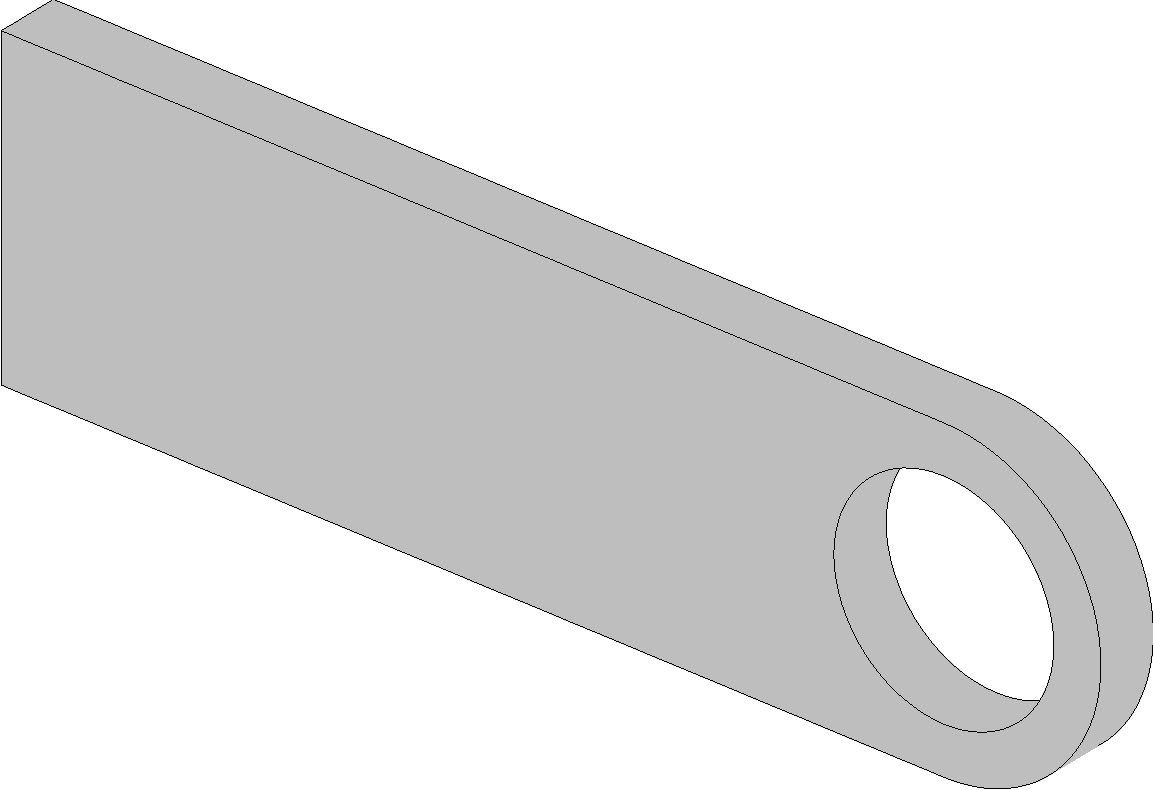
\includegraphics[width=7cm]{images/exo/1.2_geometrie}};
        \begin{scope}[x={(image.south east)},y={(image.north west)}]
          \draw[latex-latex,thick,<->] (0,0.45) -- (0.82,-0.05) node[midway,fill=white]{30~cm};
          \draw[latex-latex,thick,<->] (-0.06,0.51) -- (-0.06,0.96) node[midway,fill=white]{10~cm};
          \draw[thick,<->] (0,1) -- (0.05,1.05);
          \draw (0.07,1.1) node[anchor=north west] {2~cm};
          \draw[thick,->] (0.82,0.25) -- (0.75,0.4);
          \draw (0.75,0.4) node[anchor=south east] {3,5~cm};
          \draw[dotted,thick] (0.82,-0.1) -- (0.82,0.3);
        \end{scope}
      \end{tikzpicture}
    \end{center}
    \normalsize
  \end{itemize}
\end{frame}

\begin{frame}{\fe{1.1 Maillage non structuré}{1.1 Unstructured mesh}}
  \begin{itemize}
    \item \fe{Objectif : créer un \g{maillage paramétré} de la structure}
             {Objective: to create a \g{parametered mesh} of the structure}
    \begin{itemize}
      \item[] $\Rightarrow$ \fe{maillage non structuré}{unstructured grid}
      \item[] $\Rightarrow$ \fe{paramètre : taille de maille globale}
                              {parameter: average element size}
      \item[] $\Rightarrow$ \fe{éléments triangles/tétraèdres}{triangles/tetrahedra elements}
      \item[]
    \end{itemize}
    \item \fe{Méthode :}{Method:}
    \begin{enumerate}
      \item \fe{placer des points guides}{define the main points}
      \item \fe{mailler le contour fermé}{mesh the closed border} 
      \item \fe{mailler la surface par remplissage}{mesh the internal surface by filling}
      \item \fe{mailler le volume par extrusion}{mesh the volume by extrusion}
    \end{enumerate}
  \end{itemize}
\end{frame}

\begin{frame}{\fe{1.1 Maillage non structuré}{1.1 Unstructured mesh}}
  \begin{itemize}
    \item \fe{Options générales et paramètres}{General options and parameters}
    \lstinputlisting[language=gibiane, firstline=33, lastline=40]{dgibi/formation_debutant_1_maillage.dgibi}
    \lstinputlisting[language=gibiane, firstline=56, lastline=57]{dgibi/formation_debutant_1_maillage.dgibi}
    \vspace{2cm}
    \item[] \violet{\emph{\fe{Nouveaux objets : ENTIER, FLOTTANT, MOT}
                             {New objects: ENTIER, FLOTTANT, MOT}}}
  \end{itemize}
\end{frame}

\begin{frame}{\fe{1.1 Maillage non structuré}{1.1 Unstructured mesh}}
  \begin{itemize}
    \item \fe{Création de points}{Points creation}
    \lstinputlisting[language=gibiane, firstline=59, lastline=69]{dgibi/formation_debutant_1_maillage.dgibi}
    \vspace{2cm}
    \item[] \violet{\emph{\fe{Nouvel objet : POINT}
                             {New object: POINT}}}
  \end{itemize}
\end{frame}

\begin{frame}{\fe{1.1 Maillage non structuré}{1.1 Unstructured mesh}}
  \begin{itemize}
    \item \fe{Maillage des lignes et de contours fermés}{Meshing lines and closed contours}
    \lstinputlisting[language=gibiane, firstline=71, lastline=73]{dgibi/formation_debutant_1_maillage.dgibi}
    \lstinputlisting[language=gibiane, firstline=78, lastline=84]{dgibi/formation_debutant_1_maillage.dgibi}
    \onslide<2->{
      \lstinputlisting[language=gibiane, firstline=86, lastline=86]{dgibi/formation_debutant_1_maillage.dgibi}
      \begin{textblock*}{5cm}(8.1cm,-2.6cm)
        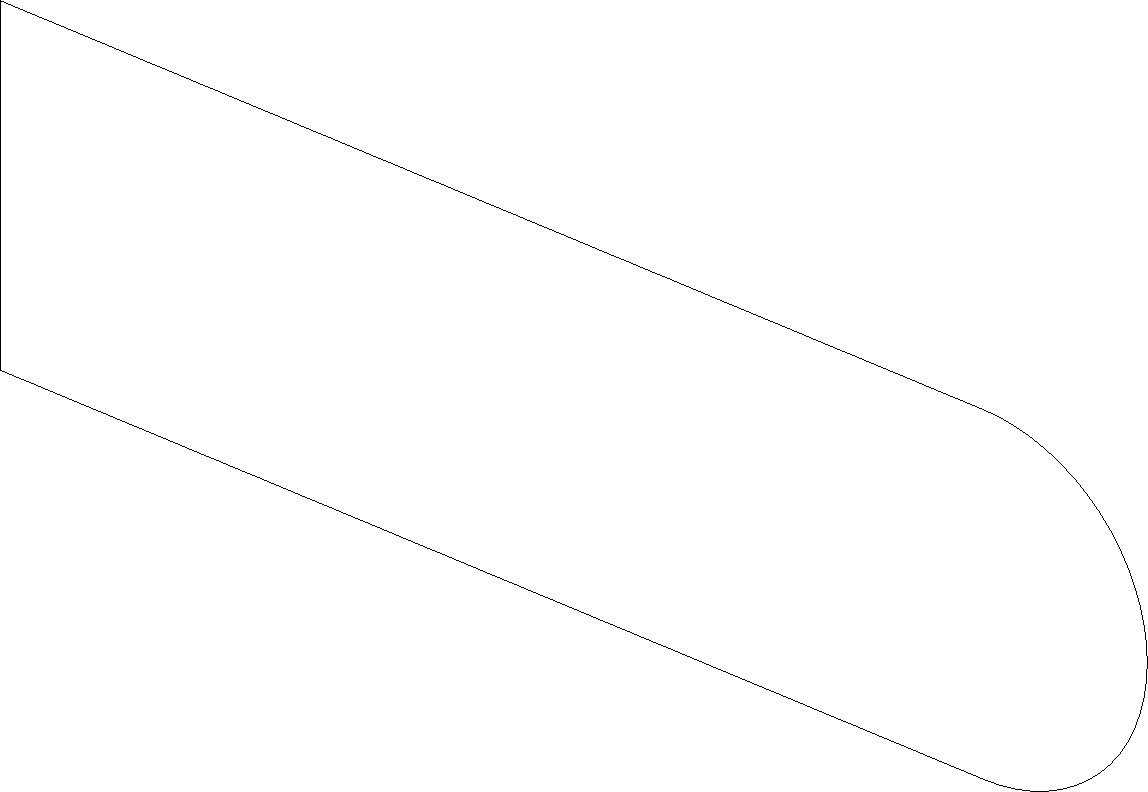
\includegraphics[width=4cm]{images/exo/1.1_maillage_tetra.01}
      \end{textblock*}}
    \onslide<3->{
      \footnotesize
      \avous{\fe{Maillage du cercle de centre p6}{Meshing the circle with center p6}}
      \normalsize}
    \onslide<4->{
      \lstinputlisting[language=gibiane, firstline=88, lastline=89]{dgibi/formation_debutant_1_maillage.dgibi}
      \lstinputlisting[language=gibiane, firstline=91, lastline=91]{dgibi/formation_debutant_1_maillage.dgibi}
      \begin{textblock*}{5cm}(8.1cm,-2.5cm)
        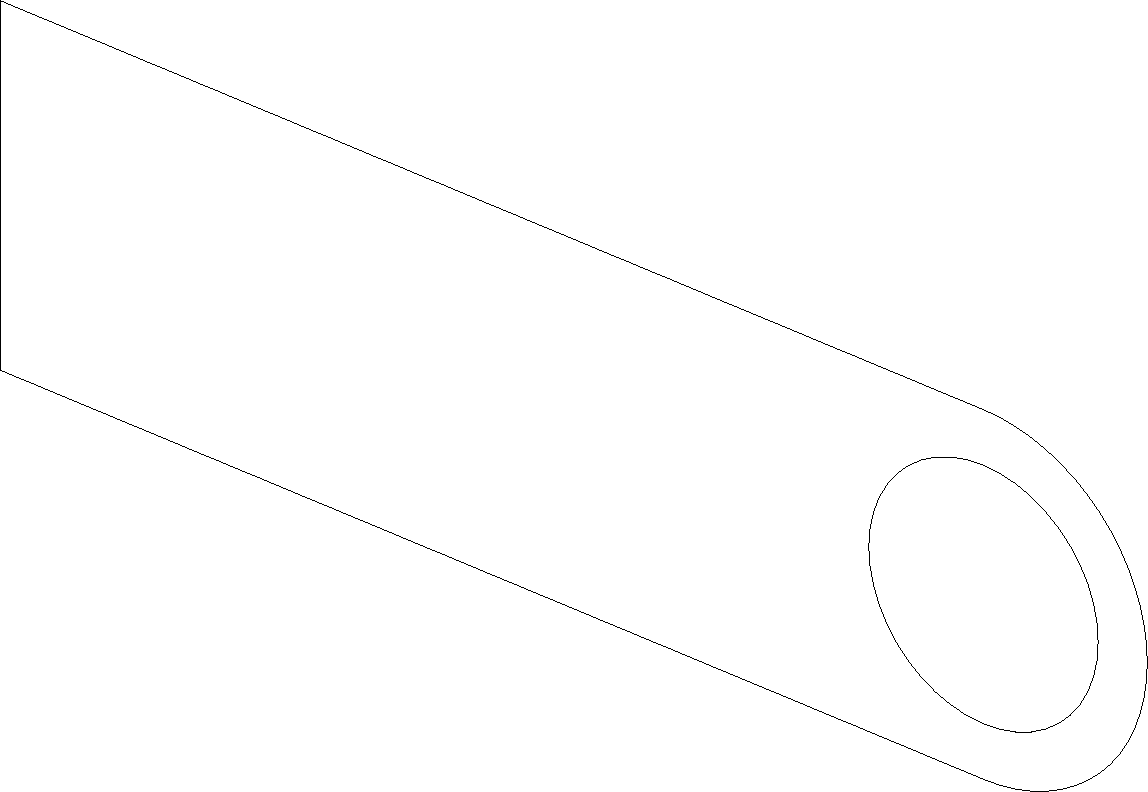
\includegraphics[width=4cm]{images/exo/1.1_maillage_tetra.02}
      \end{textblock*}}
    \item[] \violet{\emph{\fe{Nouvel objet : MAILLAGE}
                             {New object: MAILLAGE}}}
  \end{itemize}
\end{frame}

\begin{frame}{\fe{1.1 Maillage non structuré}{1.1 Unstructured mesh}}
  \begin{itemize}
    \item \fe{Maillage de la surface (maillage libre depuis le contour fermé)}
             {Surface meshing (unstructured mesh inside the closed contour)}
    \lstinputlisting[language=gibiane, firstline=93, lastline=94]{dgibi/formation_debutant_1_maillage.dgibi}
    \onslide<2->{
      \lstinputlisting[language=gibiane, firstline=96, lastline=96]{dgibi/formation_debutant_1_maillage.dgibi}}
    \onslide<2-3>{
      \begin{textblock*}{5cm}(8.1cm,-1.cm)
        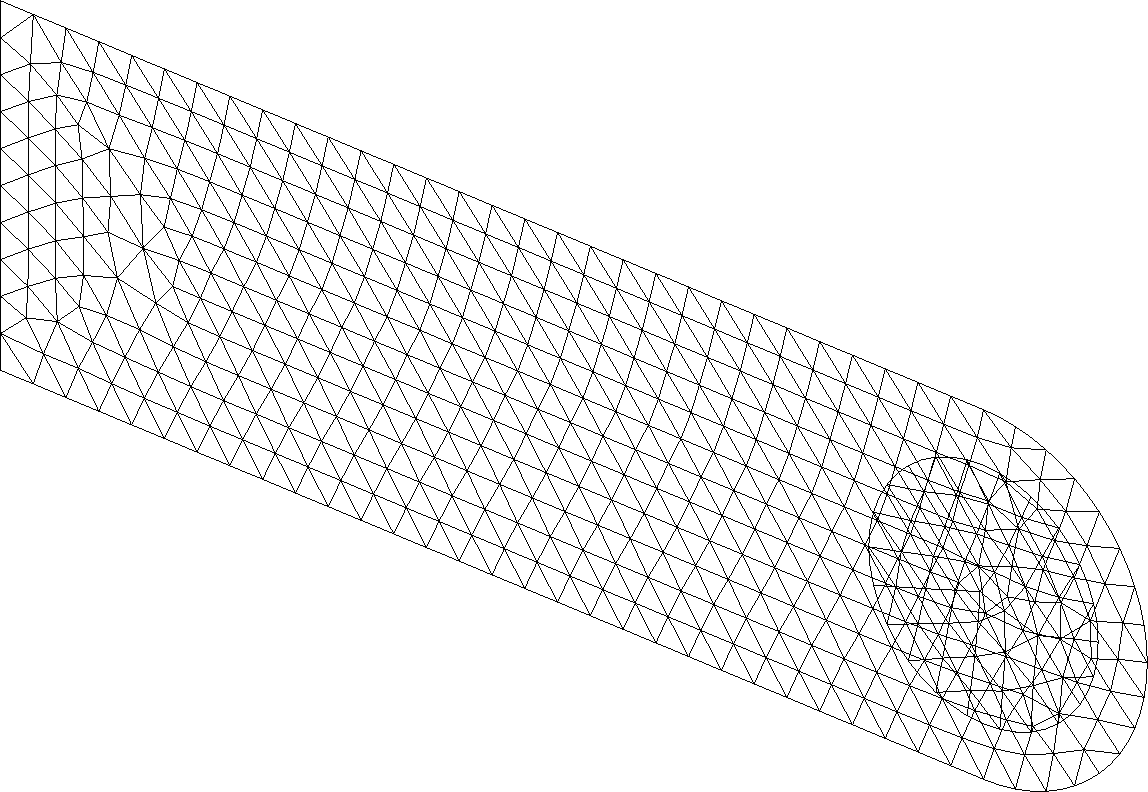
\includegraphics[width=4cm]{images/exo/1.1_maillage_tetra.03}
      \end{textblock*}}
    \onslide<3->{
      \lstinputlisting[language=gibiane, firstline=98, lastline=99]{dgibi/formation_debutant_1_maillage.dgibi}}
    \onslide<4->{
      \lstinputlisting[language=gibiane, firstline=101, lastline=101]{dgibi/formation_debutant_1_maillage.dgibi}
      \begin{textblock*}{5cm}(8.1cm,-2.5cm)
        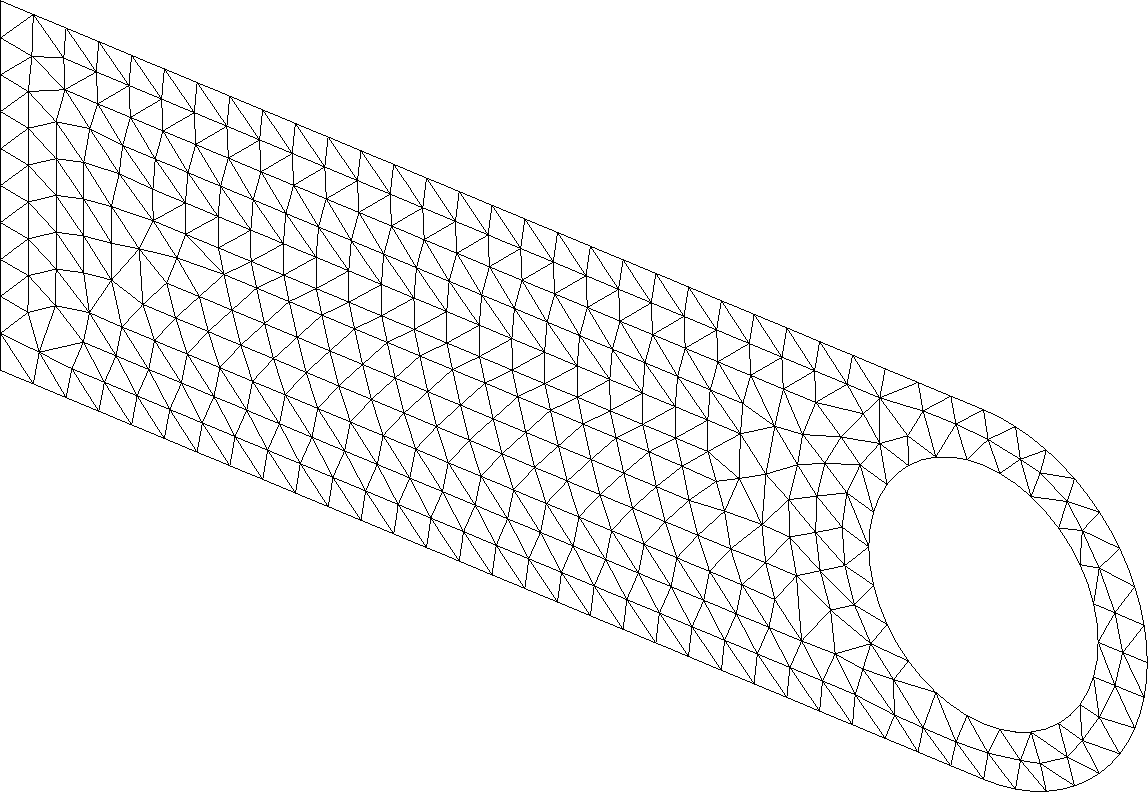
\includegraphics[width=4cm]{images/exo/1.1_maillage_tetra.04}
      \end{textblock*}}
    \item<5->\fe{Maillage du volume}{Meshing the volume}\\
    \onslide<5->{
      \footnotesize
      \avous{\fe{Mailler le volume par translation (voir : VOLU)}{Mesh the volume by translation (see: VOLU)}}
      \normalsize}
    \onslide<6->{
    \lstinputlisting[language=gibiane, firstline=103, lastline=104]{dgibi/formation_debutant_1_maillage.dgibi}}
    \onslide<6->{
      \lstinputlisting[language=gibiane, firstline=106, lastline=106]{dgibi/formation_debutant_1_maillage.dgibi}}
    \onslide<6>{
      \begin{textblock*}{5cm}(8.1cm,-2.cm)
        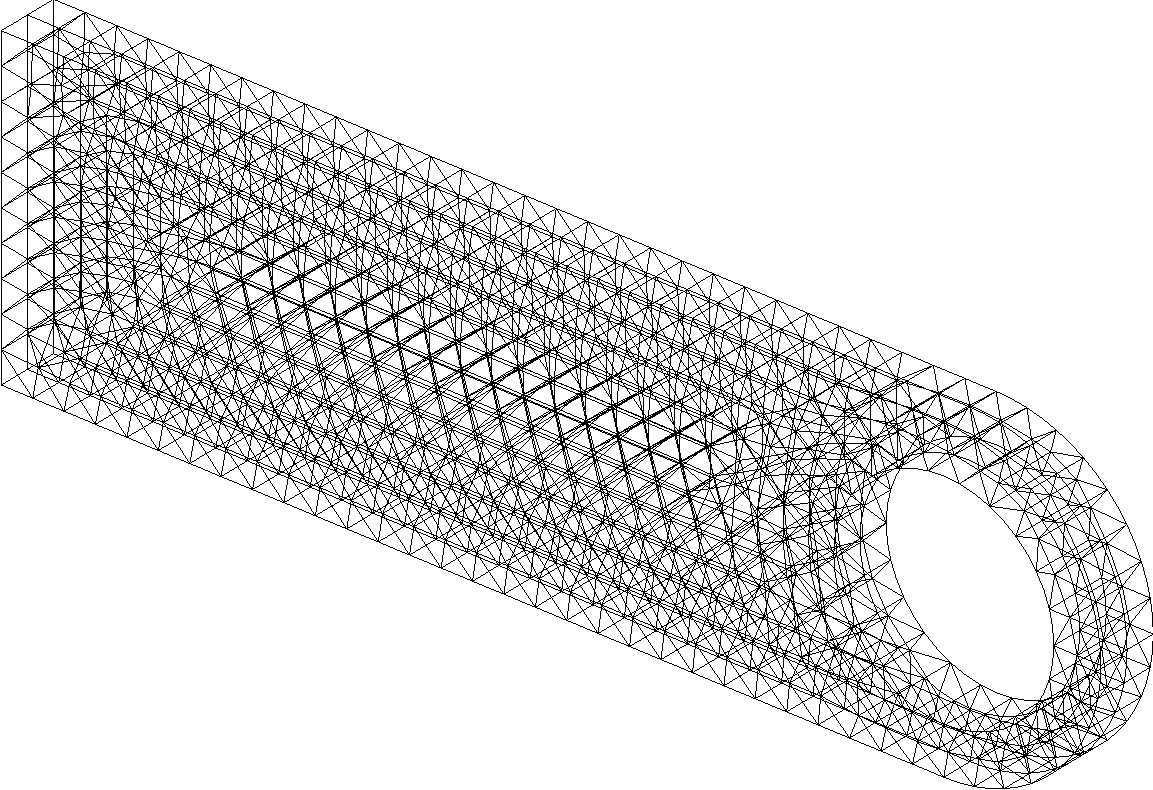
\includegraphics[width=4cm]{images/exo/1.1_maillage_tetra.05}
      \end{textblock*}}
    \onslide<7->{
      \lstinputlisting[language=gibiane, firstline=107, lastline=107]{dgibi/formation_debutant_1_maillage.dgibi}
      \begin{textblock*}{5cm}(8.1cm,-2.5cm)
        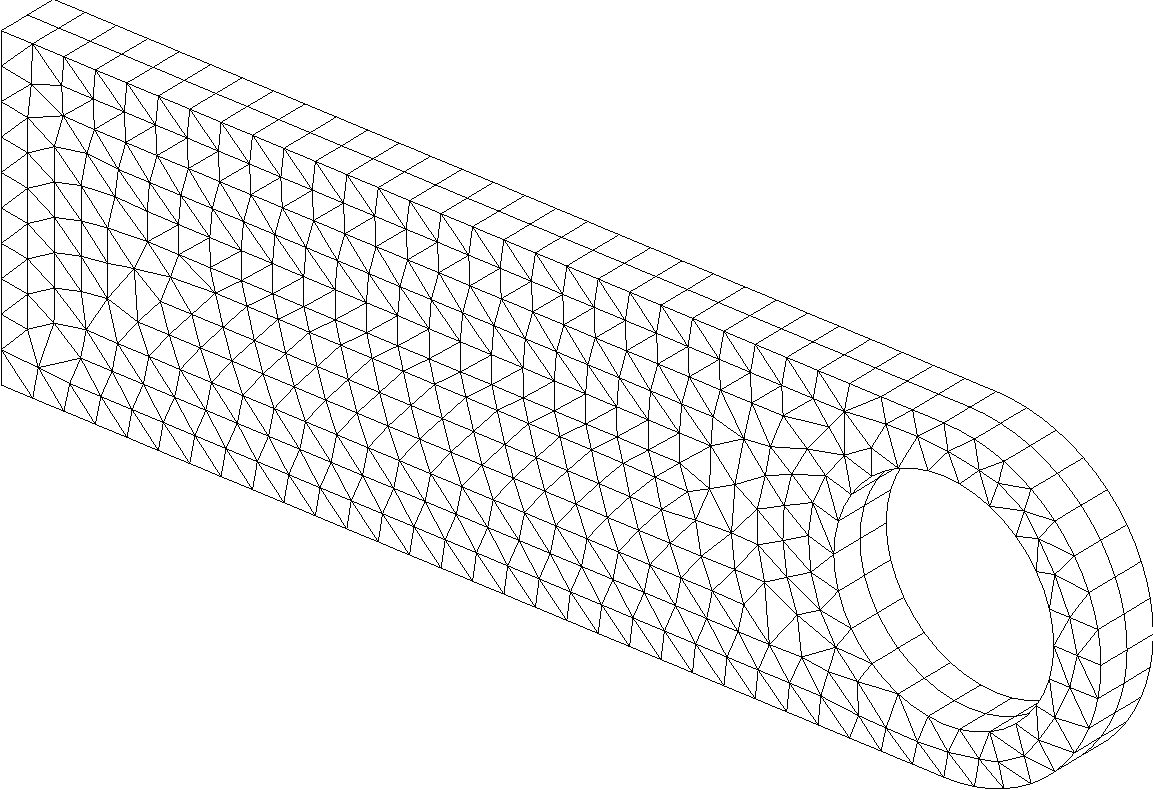
\includegraphics[width=4cm]{images/exo/1.1_maillage_tetra.06}
      \end{textblock*}}
    \item<8->\fe{Le maillage est fait de prismes !}{The mesh is made of prisms!}
  \end{itemize}
\end{frame}

\begin{frame}{\fe{1.1 Maillage non structuré}{1.1 Unstructured mesh}}
  \begin{itemize}
    \item \fe{Modification du type d'éléments}{Changing the type of elements}
    \lstinputlisting[language=gibiane, firstline=109, lastline=111]{dgibi/formation_debutant_1_maillage.dgibi}
    \lstinputlisting[language=gibiane, firstline=113, lastline=113]{dgibi/formation_debutant_1_maillage.dgibi}
    \begin{textblock*}{5cm}(8.1cm,-2.4cm)
      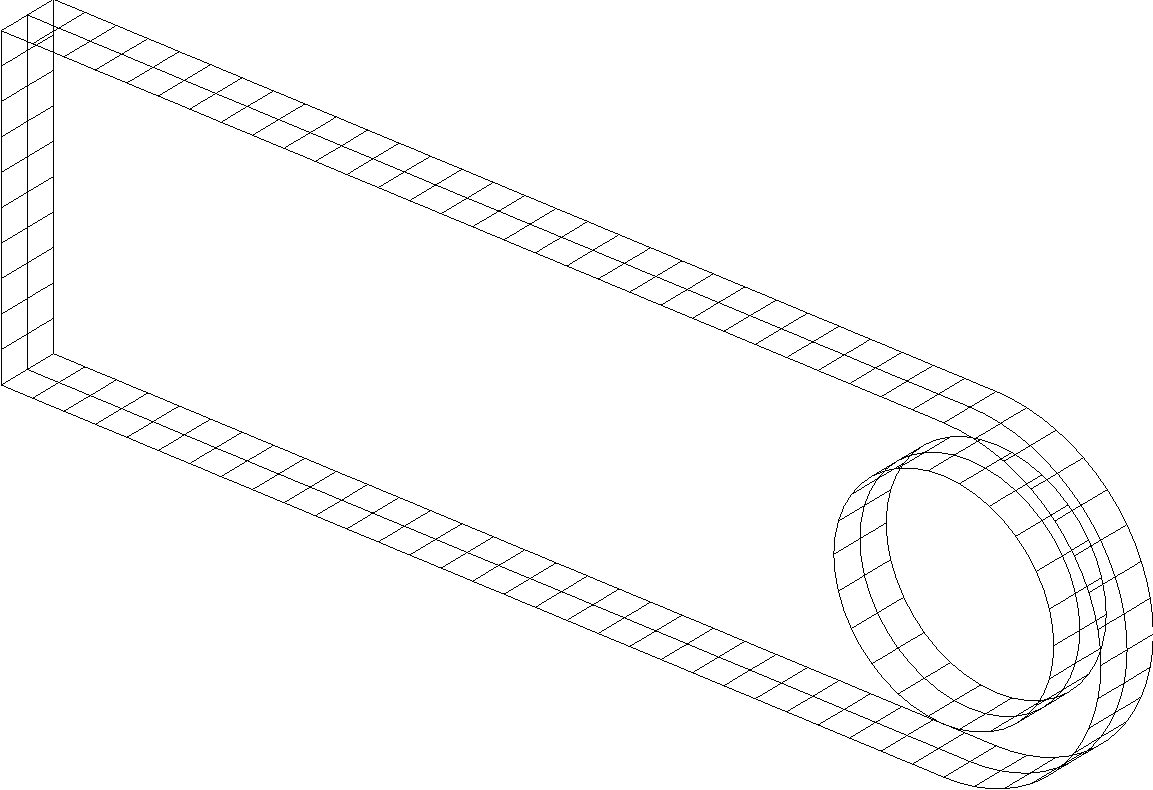
\includegraphics[width=4cm]{images/exo/1.1_maillage_tetra.07}
    \end{textblock*}
    \onslide<2->{
      \lstinputlisting[language=gibiane, firstline=115, lastline=117]{dgibi/formation_debutant_1_maillage.dgibi}}
    \onslide<3->{
      \lstinputlisting[language=gibiane, firstline=119, lastline=119]{dgibi/formation_debutant_1_maillage.dgibi}
      \begin{textblock*}{5cm}(8.1cm,-2.4cm)
        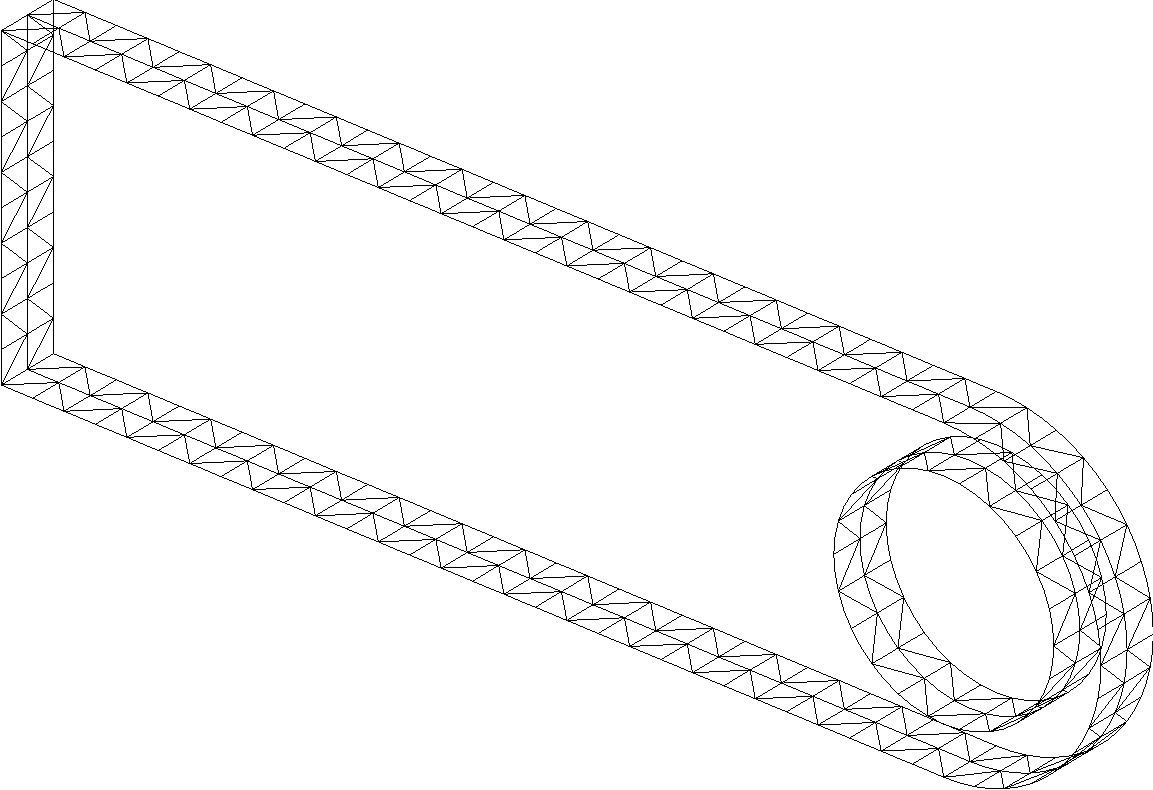
\includegraphics[width=4cm]{images/exo/1.1_maillage_tetra.08}
      \end{textblock*}}
    \onslide<4->{
      \footnotesize
      \avous{\fe{Mailler le volume dans la surface enveloppe (voir : VOLU)}
                {Mesh the volume inside the enveloppe (see: VOLU)}}
      \normalsize}
    \onslide<5->{
      \lstinputlisting[language=gibiane, firstline=121, lastline=123]{dgibi/formation_debutant_1_maillage.dgibi}
      \lstinputlisting[language=gibiane, firstline=125, lastline=125]{dgibi/formation_debutant_1_maillage.dgibi}
      \begin{textblock*}{5cm}(8.1cm,-1.8cm)
        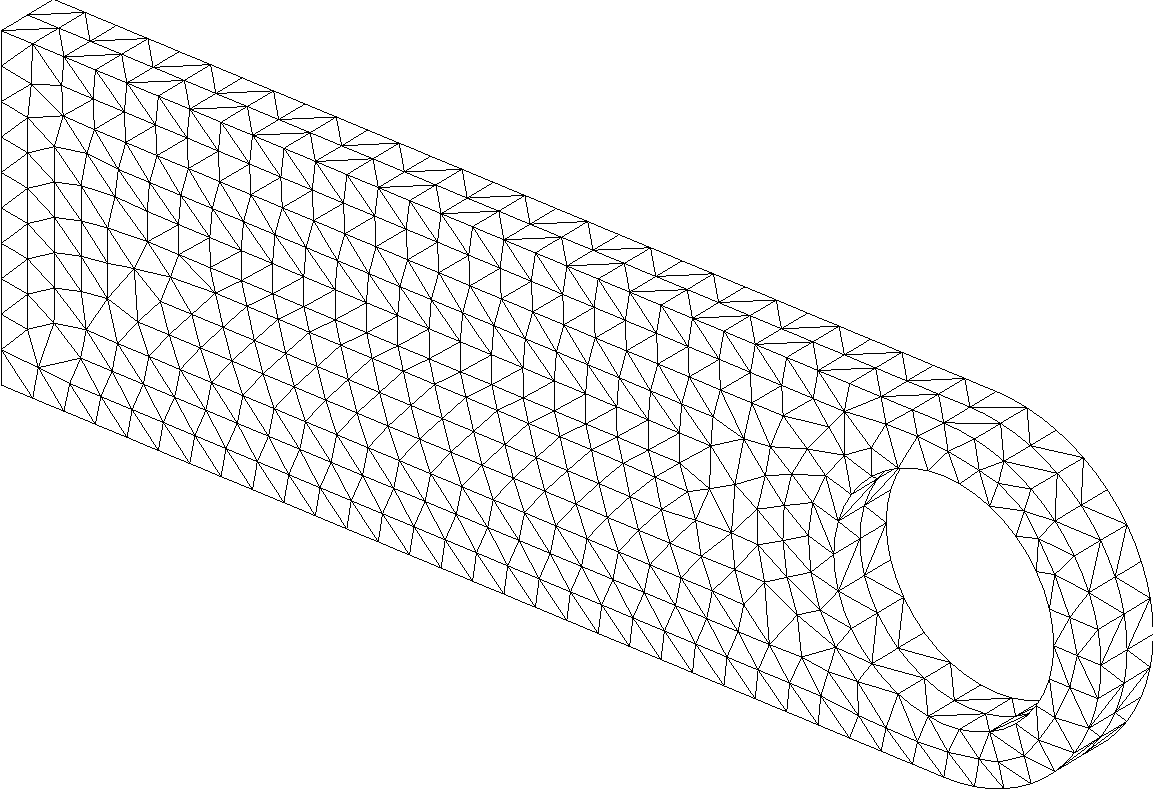
\includegraphics[width=4cm]{images/exo/1.1_maillage_tetra.09}
      \end{textblock*}}
  \end{itemize}
\end{frame}

\begin{frame}{\fe{1.2 Maillage structuré}{1.2 Structured mesh}}
  \begin{itemize}
    \item \fe{Objectif : créer un \g{maillage paramétré} de la structure}
            {Objective: to create a \g{parametered mesh} of the structure}
    \begin{itemize}
      \item[] $\Rightarrow$ \fe{maillage structuré}{structured grid}
      \item[] $\Rightarrow$ \fe{paramètre : nombre d'éléments sur les arêtes}
                              {parameter: number of elements on the edges}
      \item[] $\Rightarrow$ \fe{éléments quadrangles/hexaèdres}{quadrangles/hexahedra elements}
      \item[]
    \end{itemize}
    \item \fe{Méthode :}{Method:}
    \begin{enumerate}
      \item \fe{placer des points guides}{define the main points}
      \item \fe{mailler des lignes opposées}{mesh opposed lines}
      \item \fe{mailler des surfaces réglées}{mesh ruled surfaces}
      \item \fe{mailler le volume par extrusion}{mesh the volume by extrusion}
    \end{enumerate}
  \end{itemize}
\end{frame}

\begin{frame}{\fe{1.2 Maillage structuré}{1.2 Structured mesh}}
  \begin{itemize}
    \item \fe{Options et paramètres}{Options and parameters}
    \lstinputlisting[language=gibiane, firstline=143, lastline=145]{dgibi/formation_debutant_1_maillage.dgibi}
    \lstinputlisting[language=gibiane, firstline=150, lastline=152]{dgibi/formation_debutant_1_maillage.dgibi}
    \item<2->\fe{Maillage surfacique par translation}{Surface mesh by translation}
    \lstinputlisting[language=gibiane, firstline=154, lastline=158]{dgibi/formation_debutant_1_maillage.dgibi}
    \lstinputlisting[language=gibiane, firstline=160, lastline=160]{dgibi/formation_debutant_1_maillage.dgibi}
    \onslide<2->{
      \begin{textblock*}{5cm}(8.1cm,-2.7cm)
        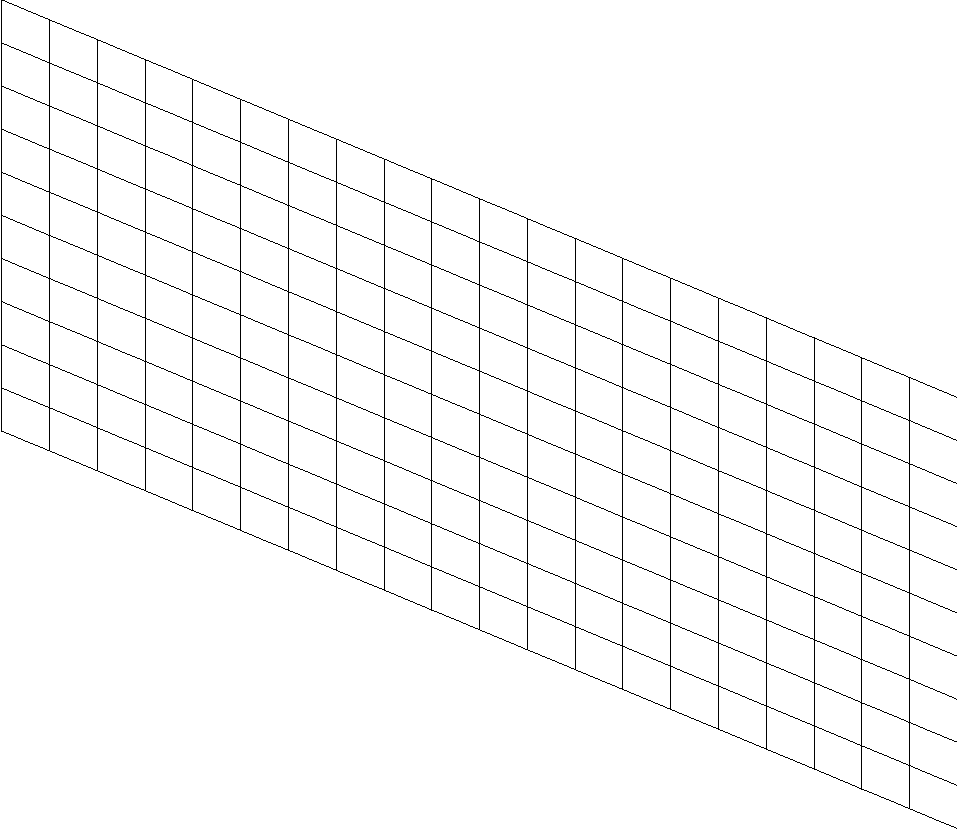
\includegraphics[width=4cm]{images/exo/1.2_maillage_hexa.1}
      \end{textblock*}}
  \end{itemize}
\end{frame}

\begin{frame}{\fe{1.2 Maillage structuré}{1.2 Structured mesh}}
  \begin{itemize}
    \item \fe{Récupération de sous zones}{Subzone recovery}
    \lstinputlisting[language=gibiane, firstline=162, lastline=166]{dgibi/formation_debutant_1_maillage.dgibi}
    \item<2->\fe{Maillage de la surface autour du trou}{Surface mesh around the hole}
    \lstinputlisting[language=gibiane, firstline=167, lastline=171]{dgibi/formation_debutant_1_maillage.dgibi}
    \onslide<3->{
      \footnotesize
      \avous{\fe{Mailler le cercle du trou par PROJection de \kw{lig1}}
                {Mesh the circle of the hole by PROJection of \kw{lig1}}}
      \normalsize}
    \onslide<4->{
    \lstinputlisting[language=gibiane, firstline=172, lastline=174]{dgibi/formation_debutant_1_maillage.dgibi}
    \lstinputlisting[language=gibiane, firstline=176, lastline=176]{dgibi/formation_debutant_1_maillage.dgibi}
      \begin{textblock*}{5cm}(9cm,-4.1cm)
        \begin{tikzpicture}
          \node[anchor=south west,inner sep=0] (image) at (0,0)
          {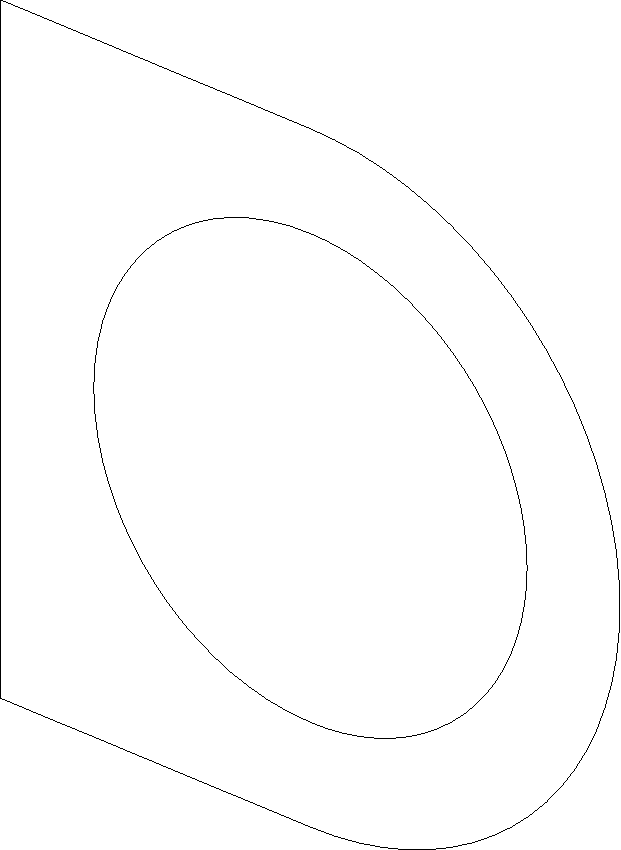
\includegraphics[width=3cm]{images/exo/1.2_maillage_hexa.2}};
          \begin{scope}[x={(image.south east)},y={(image.north west)}]
            \tiny
            \draw (0.02,0.2) node[anchor=west] {\kw{lig1}};
            \draw (0.3,0.3) node[anchor=west] {\kw{cin}};
          \end{scope}
        \end{tikzpicture}
      \end{textblock*}}
  \end{itemize}
\end{frame}

\begin{frame}{\fe{1.2 Maillage structuré}{1.2 Structured mesh}}
  \begin{itemize}
    \item \fe{Maillage de la surface réglée}{Meshing the ruled surface}\\
    \footnotesize
    \avous{\fe{Mailler la surface réglée entre \kw{cin} et \kw{lig1}\\
         \quad avec 3 éléments (voir : REGL)}
              {Mesh the ruled surface between \kw{cin} and \kw{lig1}\\
        \qquad with 3 elements (see: REGL)}}
    \normalsize
    \onslide<1-2>{
      \begin{textblock*}{5cm}(9cm,-2cm)
        \begin{tikzpicture}
          \node[anchor=south west,inner sep=0] (image) at (0,0)
          {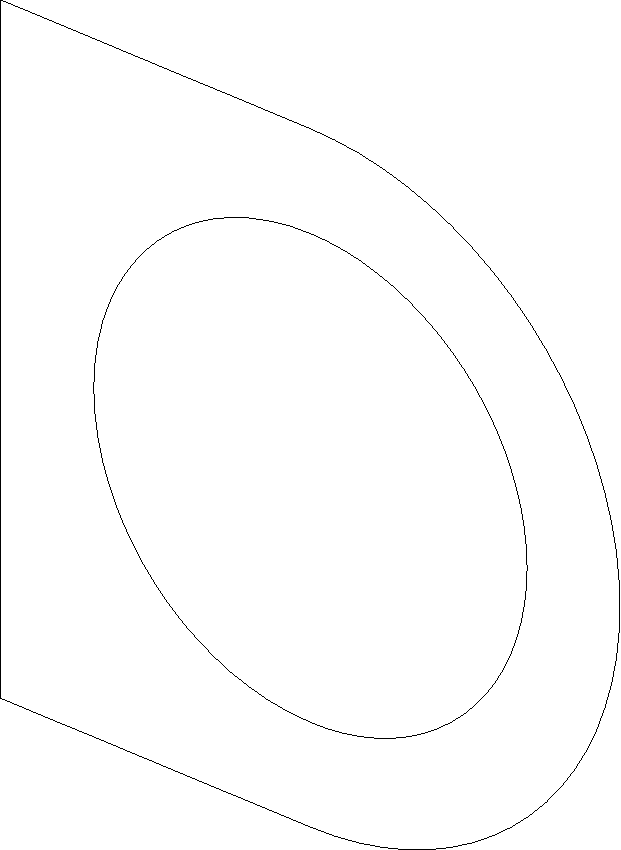
\includegraphics[width=3cm]{images/exo/1.2_maillage_hexa.2}};
          \begin{scope}[x={(image.south east)},y={(image.north west)}]
            \tiny
            \draw (0.02,0.2) node[anchor=west] {\kw{lig1}};
            \draw (0.3,0.3) node[anchor=west] {\kw{cin}};
          \end{scope}
        \end{tikzpicture}
      \end{textblock*}}
      \onslide<2->{
      \lstinputlisting[language=gibiane, firstline=178, lastline=182]{dgibi/formation_debutant_1_maillage.dgibi}}
    \onslide<3->{
      \lstinputlisting[language=gibiane, firstline=184, lastline=184]{dgibi/formation_debutant_1_maillage.dgibi}
      \begin{textblock*}{5cm}(8.1cm,-2cm)
        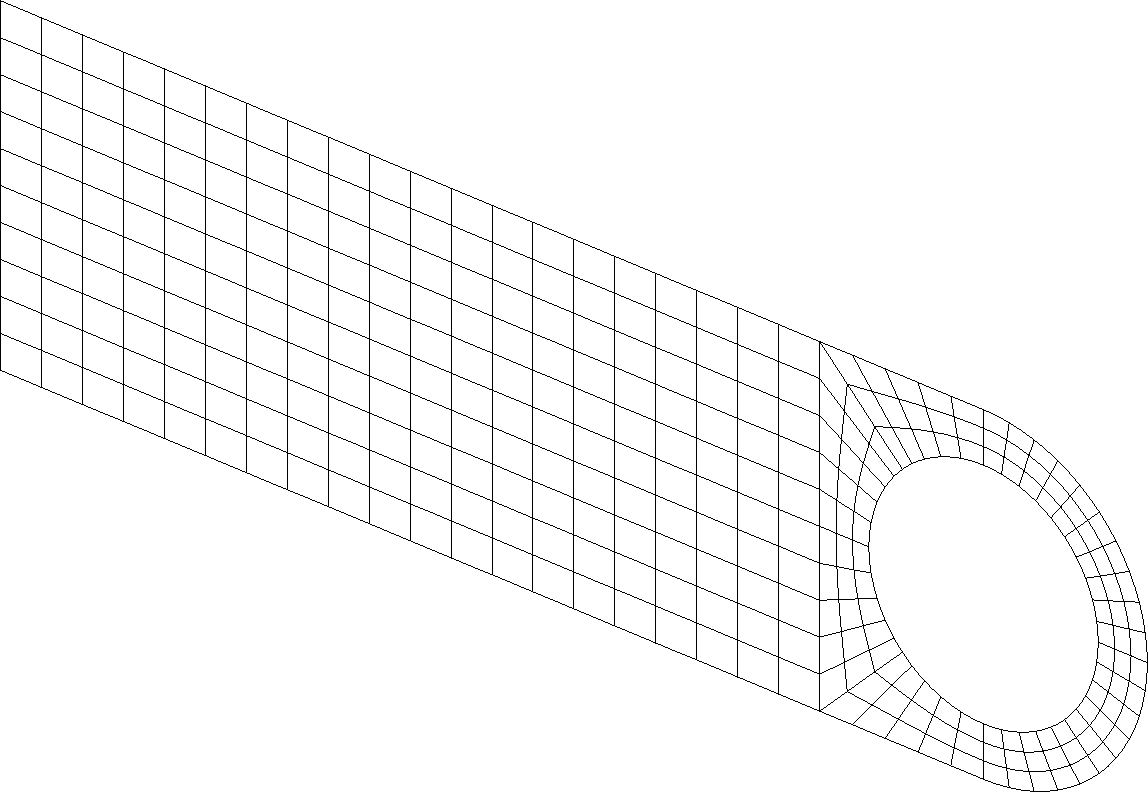
\includegraphics[width=4cm]{images/exo/1.2_maillage_hexa.3}
      \end{textblock*}}
    \item<4->\fe{Maillage du volume par translation}{Meshing the volume by translation}
    \lstinputlisting[language=gibiane, firstline=186, lastline=187]{dgibi/formation_debutant_1_maillage.dgibi}
    \lstinputlisting[language=gibiane, firstline=189, lastline=189]{dgibi/formation_debutant_1_maillage.dgibi}
    \begin{textblock*}{5cm}(8.1cm,-2cm)
      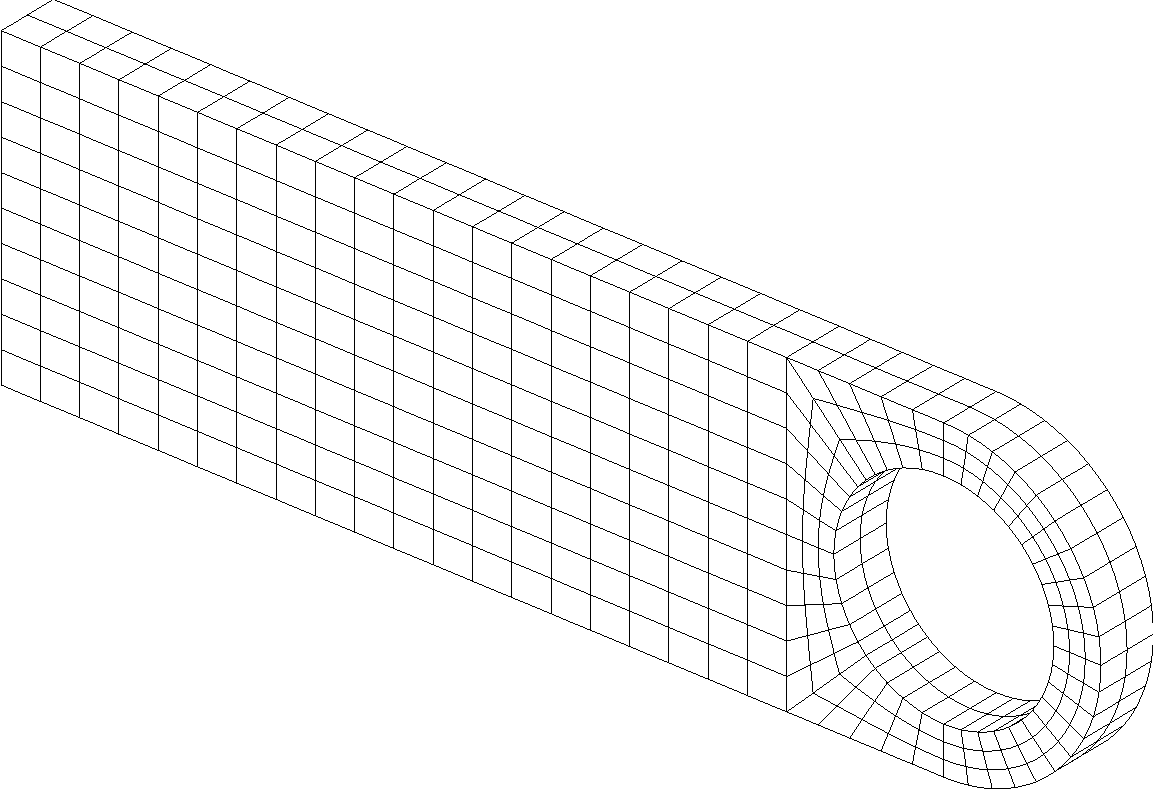
\includegraphics[width=4cm]{images/exo/1.2_maillage_hexa.4}
    \end{textblock*}
  \end{itemize}
\end{frame}

\begin{frame}{\fe{1.2 Maillage structuré}{1.2 Structured mesh}}
  \begin{itemize}
    \item \fe{Récupération de sous zones}{Subzone recovery}
    \lstinputlisting[language=gibiane, firstline=191, lastline=197]{dgibi/formation_debutant_1_maillage.dgibi}
    \item<2->\fe{Sauvegarde des données}{Saving data}
    \lstinputlisting[language=gibiane, firstline=215, lastline=218]{dgibi/formation_debutant_1_maillage.dgibi}
  \end{itemize}
\end{frame}

%%%%%%%%%%%%%%%%%%%%%%%%%%%%%%%%%%%%%%%%%%%%%%%%%%%%%%%%%%%%%%
\fe{\section{Calcul thermique}}{\section{Thermal Calculation}}
\label{thermique}
%%%%%%%%%%%%%%%%%%%%%%%%%%%%%%%%%%%%%%%%%%%%%%%%%%%%%%%%%%%%%%

\begin{frame}{On teste des trucs}
  \begin{itemize}
    \item<1->Hello
    \item<2->Comment
    \onslide<2>{\hfill\raisebox{-2cm}[0pt][0pt]{\makebox[0pt][r]{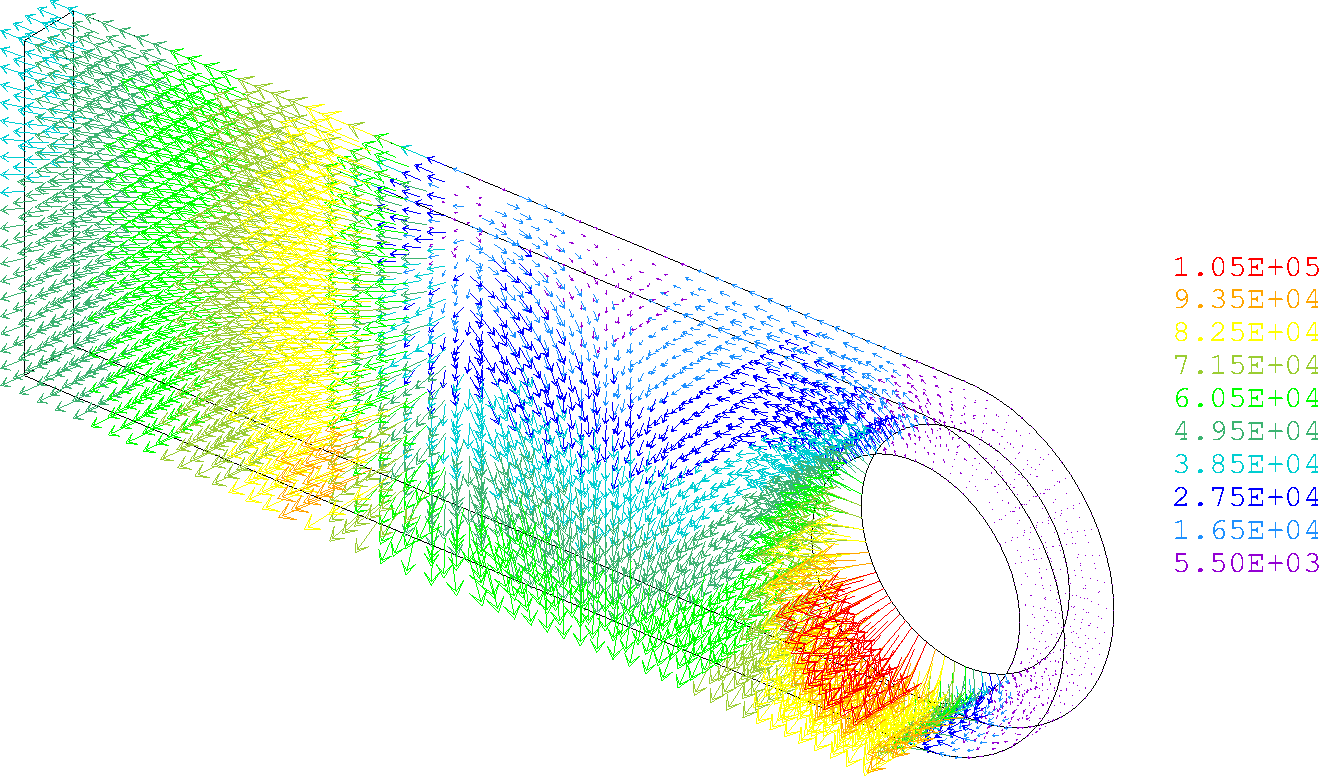
\includegraphics[height=0.5\textheight]{images/exo/4_flux}}}}
    \item<3->Ça
    \item<4->Va ?
  \end{itemize}
\end{frame}
\begin{frame}{On teste des trucs}
  \begin{itemize}
    \item<1->Hello
    \item<2->Comment
    \item<3->Ça
    \item<4->Va ?
  \end{itemize}
\end{frame}

\begin{frame}{On teste encore des trucs}
  \begin{itemize}
    \item<1->Hello
    \item<2->Comment
    \item<3->Ça
    \item<4->Va ?
  \end{itemize}
\end{frame}

\begin{frame}{On teste toujours des trucs}
  \begin{itemize}
    \item<1->Hello
    \item<2->Comment
    \item<3->Ça
    \item<4->Va ?
  \end{itemize}
\end{frame}

%%%%%%%%%%%%%%%%%%%%%%%%%%%%%%%%%%%%%%%%%%%%%%%%%%%%%%%%%%%%%%
\fe{\section{Calcul mécanique}}{\section{Mechanical Calculation}}
\label{mecanique}
%%%%%%%%%%%%%%%%%%%%%%%%%%%%%%%%%%%%%%%%%%%%%%%%%%%%%%%%%%%%%%

\fe{\subsection{Mécanique linéaire}}{\subsection{Linear Mechanics}}
\begin{frame}{\fe{Mécanique}{Mechanics}}{\fe{Rappels}{Reminders}}
  \begin{itemize}
    \item \fe{Équation d'équilibre statique}{Static equilibrium equation}
    \begin{block}{\fe{Forme locale}{Local form}}
      \begin{equation*}
        \tx{div}(\tod{\sigma})+\tou{f}=\tou{0}\quad\fe{\tx{sur }V}{\tx{on }V}
      \end{equation*}
    \end{block}~
    \item \fe{Conditions aux limites}{Boundary conditions}\\
    \footnotesize
%    \setlength\tabcolsep{1.5pt}
    \fe{\begin{tabular}{lrll}
          Déplacements imposés & $\tou{u}$              & $=\tou{u}_{\tx{imp}}$ & sur $\partial V_u$\\
          Efforts imposés      & $\tod{\sigma}.\tou{n}$ & $=\tou{t}_{\tx{imp}}$ & sur $\partial V_t$\\
        \end{tabular}}
       {\begin{tabular}{lrll}
          Imposed displacements & $\tou{u}$              & $=\tou{u}_{\tx{imp}}$ & on $\partial V_u$\\
          Imposed forces        & $\tod{\sigma}.\tou{n}$ & $=\tou{t}_{\tx{imp}}$ & on $\partial V_t$\\
        \end{tabular}}
    \normalsize
    \item \fe{Avec}{With}
    \begin{itemize}
      \item[] $\tou{u}$ \fe{vecteur déplacement}{displacement vector}
      \item[] $\tod{\sigma}$ \fe{tenseur des contraintes}{stress tensor}
      \item[] $\tou{f}$ \fe{vecteur des forces volumiques}{volumic forces vector}
      \item[] $\tou{n}$ \fe{vecteur normal à la surface}{normal vector to a surface}
    \end{itemize}
    \normalsize
  \end{itemize}
\end{frame}

\begin{frame}{\fe{Mécanique}{Mechanics}}{\fe{Rappels}{Reminders}}
  \small
  \begin{itemize}
    \item \fe{Éléments finis :}{Finite elements:} $\tou{u}(x)=[N(x)]\{U\}$
    \begin{block}{\fe{Formulation faible et discrétisée de l'équilibre :}
                     {Weak and discrete formulation of equilibrium:}}
      \begin{equation*}
        \int_{V}[B]^T\{\sigma\}dV=\{F\}
      \end{equation*}
    \end{block}~\\
    \footnotesize
    \begin{center}
      $\underbrace{\int_{V}[B]^T\{\sigma\}dV}_{[B]\{\sigma\}}=\underbrace{\int_{\partial V_t}[N]^T\{t\}_{\tx{imp}}dS}_{\{F\}_{\tx{s}}}+\underbrace{\int_{\partial V_u}[N]^T\{\sigma .n\}dS}_{\{F\}_{\tx{reac}}}+\underbrace{\int_{V}[N]^T\{f\}_{\tx{s}}dV}_{\{F\}_{\tx{v}}}$
    \end{center}
    \scriptsize
    \fe{Vecteurs de forces nodales équivalentes aux :}{Equivalent nodal forces vector to:}
    \scriptsize
    \begin{tabular}{ll}
      $\{F\}_{\tx{s}}$    & \fe{densité surfacique d'efforts imposés $\tou{t}_{\tx{imp}}$}
                               {imposed surface forces $\tou{t}_{\tx{imp}}$}\\
      $\{F\}_{\tx{reac}}$ & \fe{densité surfacique de réaction aux déplacements imposés $\tou{u}_{\tx{imp}}$}
                               {surface reactions to imposed displacements $\tou{u}_{\tx{imp}}$}\\
      $\{F\}_{\tx{v}}$    & \fe{densité volumique d'efforts imposés $\tou{f}_{\tx{imp}}$}{imposed volume forces $\tou{f}_{\tx{imp}}$}\\
      $[B]\{\sigma\}$     & \fe{densité volumique d'efforts intérieurs}{internal volume forces}
    \end{tabular}\\
    \fe{Matrices :}{Matrices:}\\
    \begin{tabular}{ll}
      $[N]$ & \fe{matrice des fonctions de forme}{matrix of shape functions}\\
      $[B]$ & \fe{matrice des dérivées des fonctions de forme}{matrix of derivative of shape functions}
     \end{tabular}
  \end{itemize}
  \normalsize
\end{frame}

\begin{frame}{\fe{Mécanique}{Mechanics}}{\fe{Rappels}{Reminders}}
  \begin{itemize}
    \item \fe{Hypothèse des petites déformations :}{Infinitesimal strains hypothesis:} $\{\varepsilon\}=[B]\{U\}$
    \item \fe{Élasticité linéaire :}{Linear elasticity:} $\{\sigma\}=[C]\{\varepsilon\}$
    \begin{block}{\fe{Formulation faible et discrétisée de l'équilibre :}
                     {Weak and discrete formulation of equilibrium:}}
      \begin{equation*}
        \underbrace{\int_{V}[B]^T[C][B]dV}_{[K]}\{U\}=\{F\}
      \end{equation*}
    \end{block}~\\
    \fe{Matrices :}{Matrices:}\\
    \begin{tabular}{ll}
      $[C]$ & \fe{matrice de Hooke}{Hooke matrix}\\
      $[K]$ & \fe{matrice de rigidité}{stifness matrix}
    \end{tabular}
  \end{itemize}
\end{frame}

\begin{frame}{\fe{6 Problème étudié}{6 Problem description}}
  \begin{itemize}
    \item \fe{Élasticité linéaire}{Linear elasticity}
    \begin{center}
    \footnotesize
    \begin{tikzpicture}
      \node[anchor=south west,inner sep=0] (image) at (0,0)
      {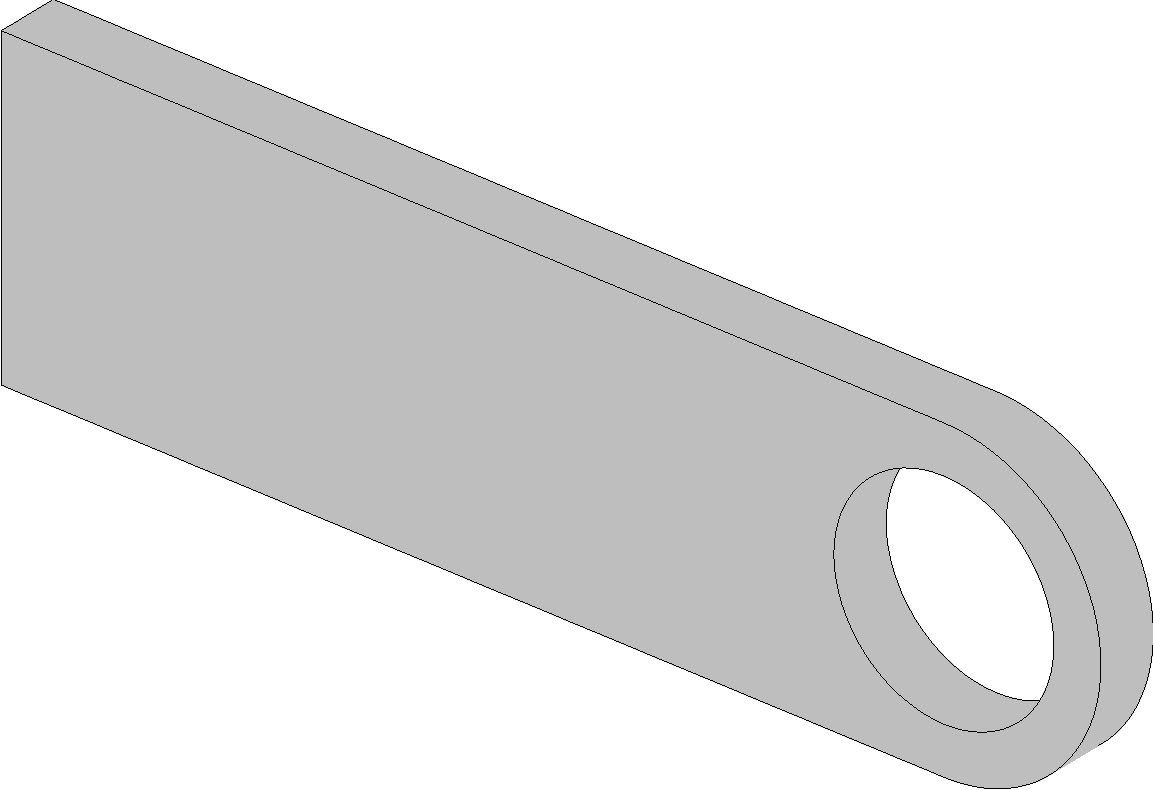
\includegraphics[width=4cm]{images/exo/1.2_geometrie}};
      \begin{scope}[x={(image.south east)},y={(image.north west)}]
        \draw (1,0.9) node[anchor=west] {$E$~=~200~GPa};
        \draw (1,0.7) node[anchor=west] {$\nu$~=~0.3};
        \draw (1,0.5) node[anchor=west] {$\alpha$~=~10$^{-5}$~K$^{-1}$};
      \end{scope}
    \end{tikzpicture}
    \normalsize
    \end{center}
    \begin{columns}
      \begin{column}{.4\textwidth}
        \item \fe{Déplacements imposés}{Imposed displacements}
        \footnotesize
        \begin{tikzpicture}
          \node[anchor=south west,inner sep=0] (image) at (0,0)
          {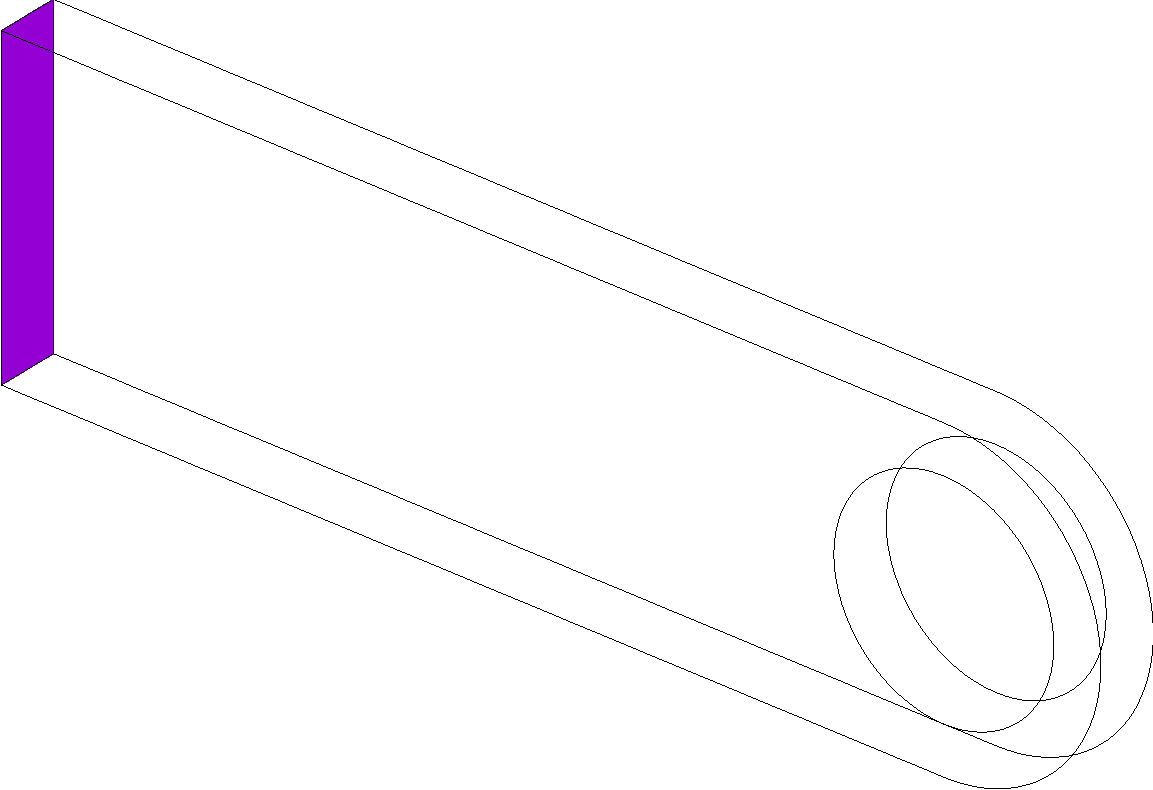
\includegraphics[width=3.5cm]{images/exo/6_cl_deplacement}};
          \begin{scope}[x={(image.south east)},y={(image.north west)},color=violet]
            \draw (0.06,0.7) node[anchor=north west] {$u_x=u_y=u_z$~=~0~m};
          \end{scope}
        \end{tikzpicture}
        \normalsize
      \end{column}
      \begin{column}{.4\textwidth}
        \item \fe{Forces imposées}{Imposed forces}
        \footnotesize
        \begin{tikzpicture}
          \node[anchor=south west,inner sep=0] (image) at (0,0)
          {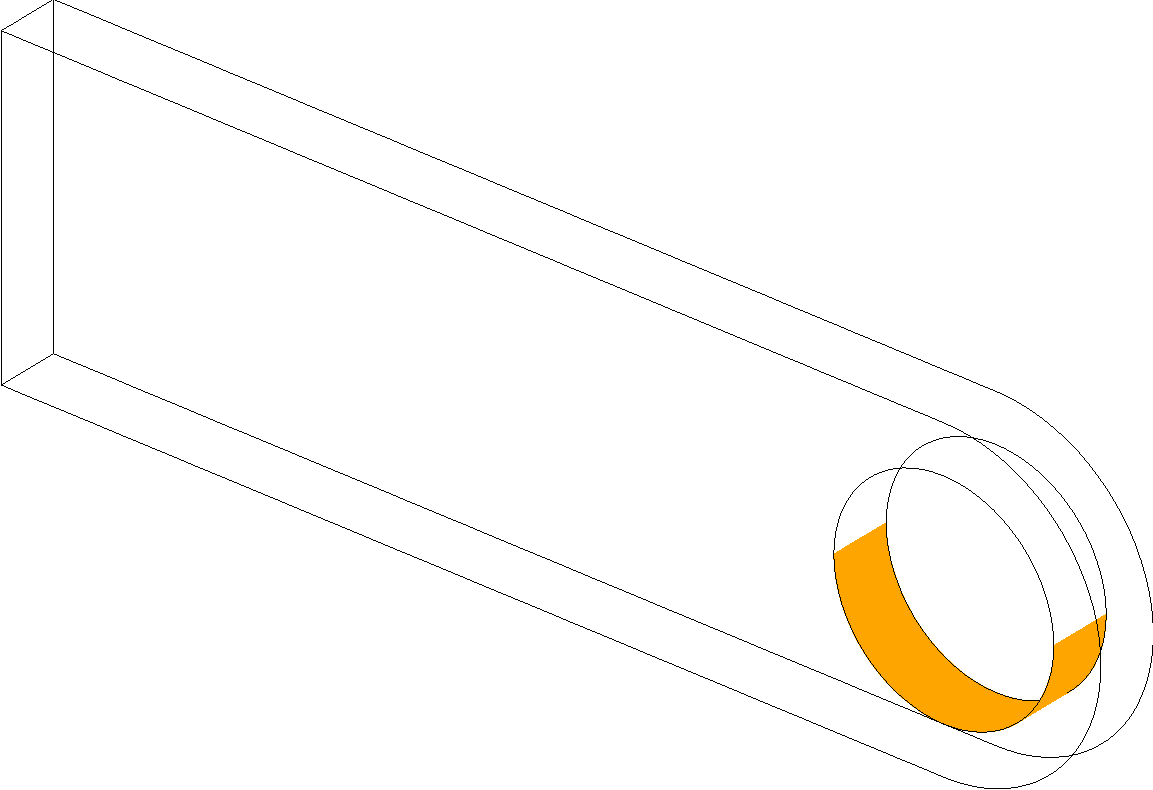
\includegraphics[width=3.5cm]{images/exo/6_cl_force}};
          \begin{scope}[x={(image.south east)},y={(image.north west)},color=orange]
            \draw (0.8,0.75) node[anchor=north west] {\fe{masse suspendue}{hanging mass}};
            \draw (0.9,0.6) node[anchor=north west] {$m$~=~2500~kg};
          \end{scope}
        \end{tikzpicture}
        \normalsize
      \end{column}
    \end{columns}
  \end{itemize}
\end{frame}

\begin{frame}{\fe{6 Mécanique linéaire}{6 Linear mechanics}}
             {\fe{Élasticité}{Elasticity}}
  \begin{itemize}
    \item \fe{Objectif : calcul mécanique linéaire\\
              en déplacements et forces imposées}
            {Objective: linear mechanical calculation\\
             with fixed displacements and forces}
    \begin{center}
      $[K]\{U\}=\{F\}$ \qquad $\Rightarrow$ \fe{Système linéaire}{Linear system}
    \end{center}
    \item \fe{Méthode :}{Method:}\\
    \begin{tabular}{ll}
      \fe{calcul de la matrice de rigidité}{stiffness matrix calculation} & $[K]$\\
      \fe{calcul des chargement nodaux équivalents}{fixed nodal forces loads calculation} & $\{F\}$\\
      \fe{résolution avec \kwr{RESO}}{sovling with \kwr{RESO}} & $\{U\}=[K]^{-1}\{F\}$
    \end{tabular}
  \end{itemize}
\end{frame}



\begin{frame}{\fe{6 Mécanique linéaire}{6 Linear mechanics}}
             {\fe{Élasticité}{Elasticity}}
  \begin{itemize}
    \item \fe{Restitution des objets (maillage, paramètres, …)}
             {Input data from previous computation (mesh, parameters, …)}
    \lstinputlisting[language=gibiane, firstline=28, lastline=29]{dgibi/formation_debutant_3_mecanique.dgibi}
    \item \fe{Nouveaux paramètres}{New parameters}
    \lstinputlisting[language=gibiane, firstline=42, lastline=45]{dgibi/formation_debutant_3_mecanique.dgibi}
    \lstinputlisting[language=gibiane, firstline=48, lastline=50]{dgibi/formation_debutant_3_mecanique.dgibi}
  \end{itemize}
\end{frame}

\begin{frame}{\fe{6 Mécanique linéaire}{6 Linear mechanics}}
             {\fe{Élasticité}{Elasticity}}
  \begin{itemize}
    \item \fe{Formulation mathématique (élasticité)}{Mathematical formulation (elasticity)}
    \lstinputlisting[language=gibiane, firstline=68, lastline=71]{dgibi/formation_debutant_3_mecanique.dgibi}
    \item<2->\fe{Matrice de rigidité}{Stifness matrix}
    \onslide<2->{
      \lstinputlisting[language=gibiane, firstline=73, lastline=74]{dgibi/formation_debutant_3_mecanique.dgibi}
      \begin{flushright}
        \footnotesize
        $[K]=\int_V[B]^T[C][B]dV$
        \normalsize
      \end{flushright}}
    \item<3->\fe{Conditions aux limites}{Boundary conditions}
    \onslide<3->{
      \lstinputlisting[language=gibiane, firstline=76, lastline=77]{dgibi/formation_debutant_3_mecanique.dgibi}}
  \end{itemize}
\end{frame}

\begin{frame}{\fe{6 Mécanique linéaire}{6 Linear mechanics}}
             {\fe{Élasticité}{Elasticity}}
  \begin{itemize}
    \item \fe{Comment représenter le chargement ?}{How to represent the load?}
    \only<1>{\vspace{7cm}}
    \only<2-4>{
    \item \fe{1) Avec une \g{\tou{force ponctuelle}}}{1) With a \g{\tou{single point force}}}\\
    \begin{textblock*}{5cm}(8.7cm,-2.4cm)
      \begin{tikzpicture}
        \scriptsize
        \node[anchor=south west,inner sep=0] (image) at (0,0)
        {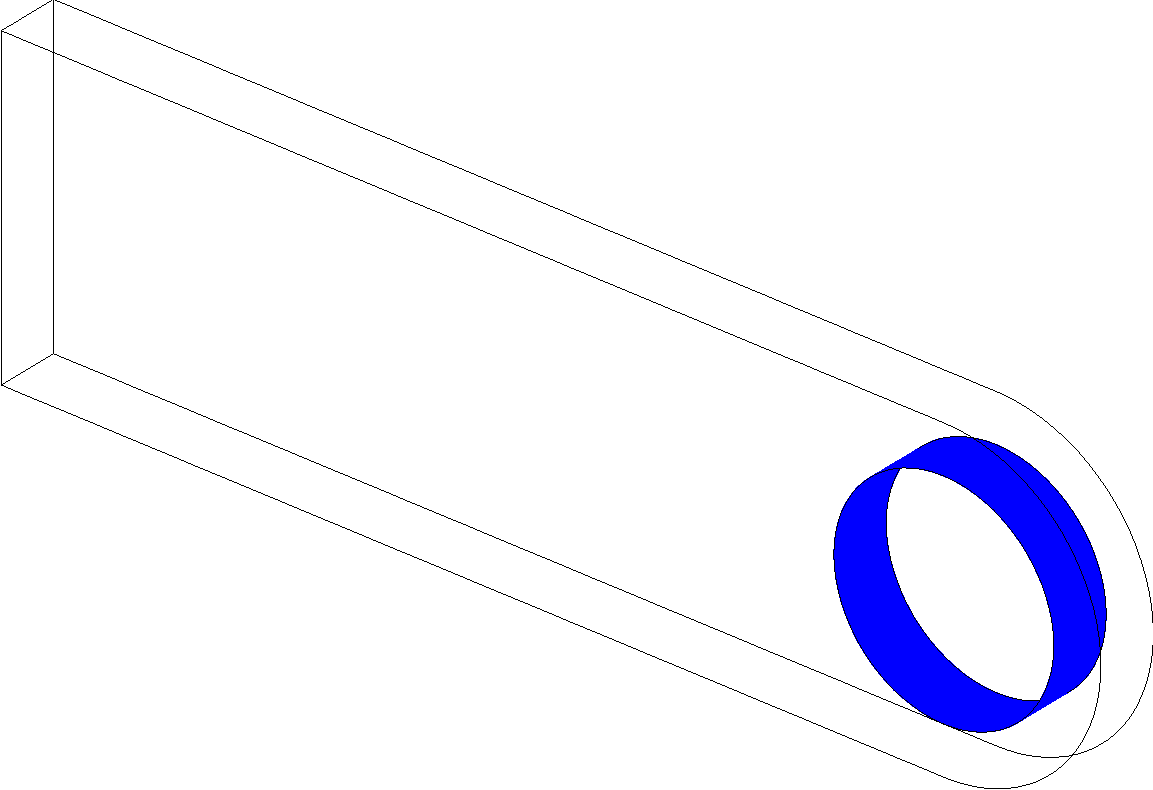
\includegraphics[width=3.5cm]{images/exo/2.1_cl_temperature}};
        \begin{scope}[x={(image.south east)},y={(image.north west)}]
          \draw (0.85,0.5) node {\kwb{sint}};
          \filldraw[black] (0.85,0.1) circle (1pt) node[anchor=north]{\kw{ptmass}};
        \end{scope}
      \end{tikzpicture}
    \end{textblock*}
    \avous{\fe{Récupérer le "centre" de la surface (voir : POIN 'PROC')}
              {Get the "center" of the surface (see: POIN 'PROC')}}\\
    \avous{\fe{Appliquer une force ponctuelle (voir : FORC)}
              {Apply a single point force (see: FORC)}}
    \onslide<3-4>{
      \lstinputlisting[language=gibiane, firstline=88, lastline=89]{dgibi/formation_debutant_3_mecanique.dgibi}}
    \onslide<4>{
      \lstinputlisting[language=gibiane, firstline=90, lastline=90]{dgibi/formation_debutant_3_mecanique.dgibi}
      \lstinputlisting[language=gibiane, firstline=95, lastline=95]{dgibi/formation_debutant_3_mecanique.dgibi}
      \begin{textblock*}{5cm}(7.8cm,-0.5cm)
        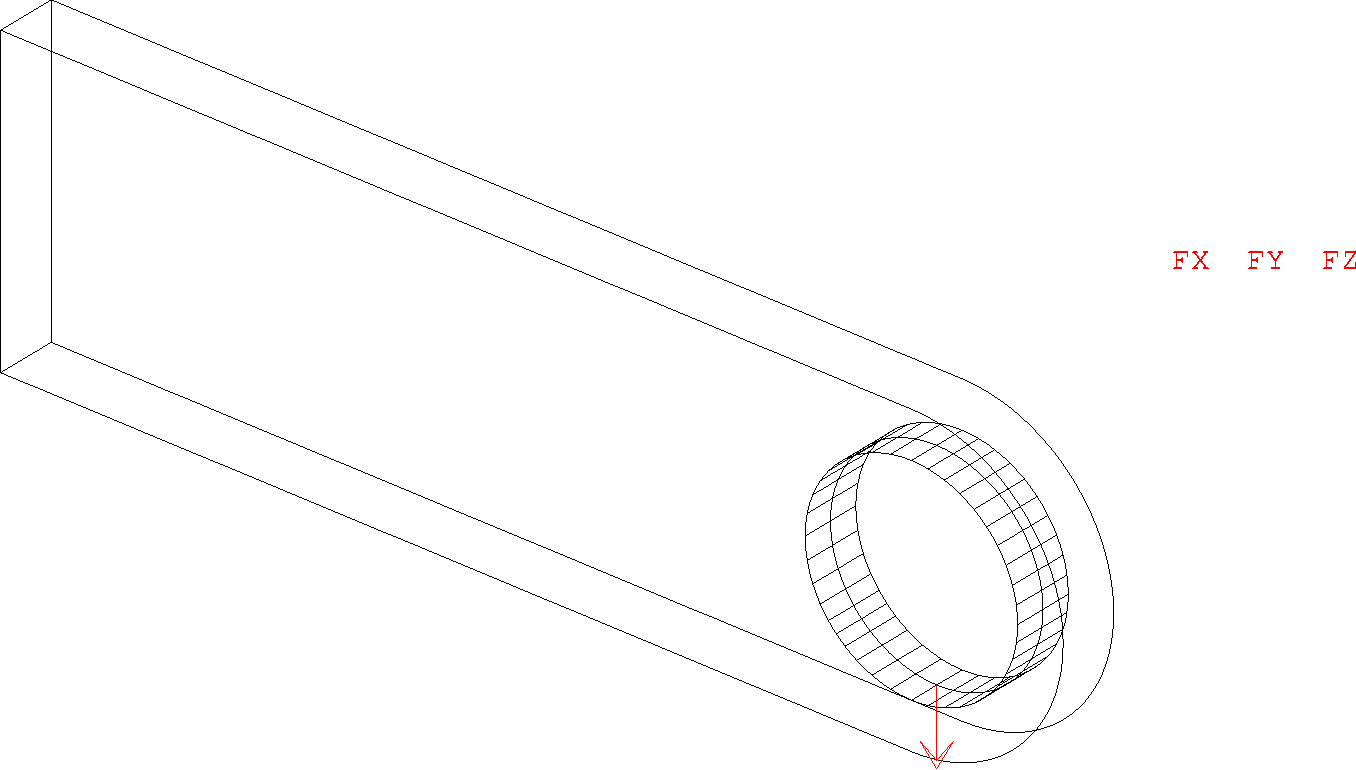
\includegraphics[width=4.5cm]{images/exo/6_forces.1}
      \end{textblock*}}
    \vspace{5cm}
    }
    \only<5-7>{
    \item \fe{2) Avec une \g{\tou{pression}}}{2) With a \g{\tou{pressure}}}\\
    \begin{textblock*}{5cm}(8.7cm,-2.4cm)
      \begin{tikzpicture}
        \scriptsize
        \node[anchor=south west,inner sep=0] (image) at (0,0)
        {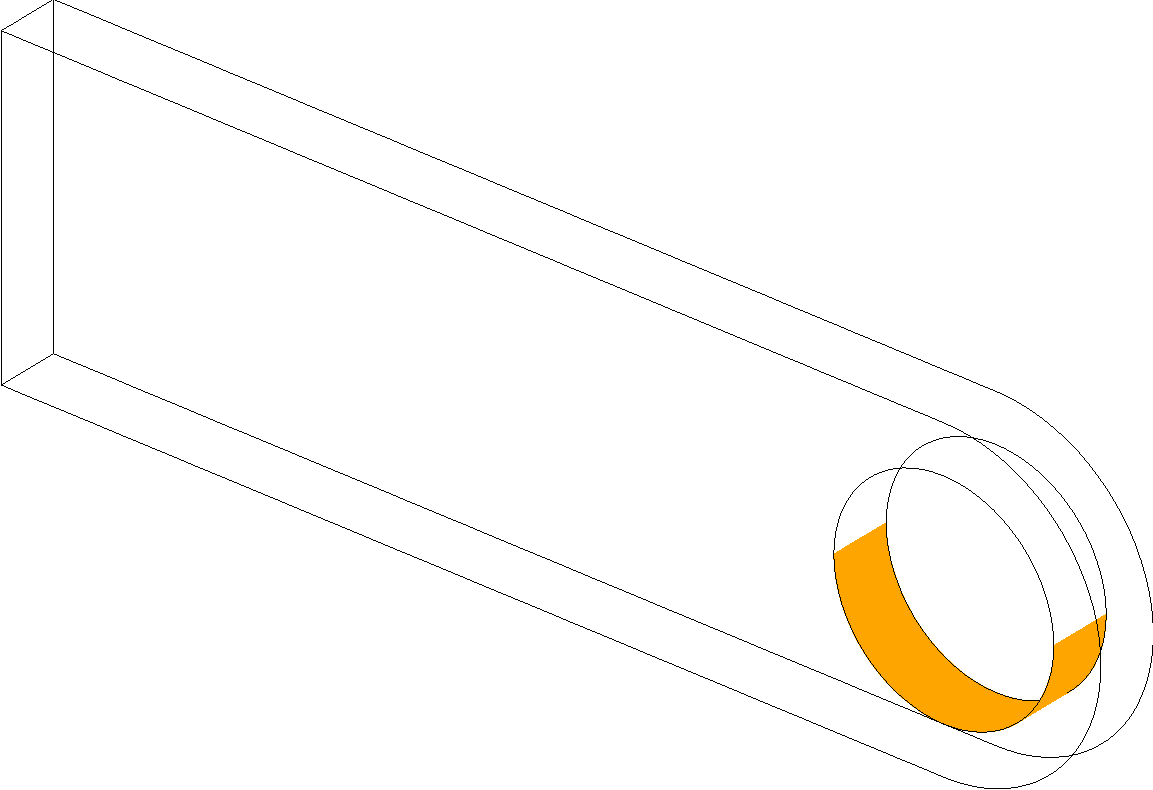
\includegraphics[width=3.5cm]{images/exo/6_cl_force}};
        \begin{scope}[x={(image.south east)},y={(image.north west)}]
          \draw (0.85,0.03) node {\orange{\kw{elmass}}};
        \end{scope}
      \end{tikzpicture}
    \end{textblock*}
    \avous{\fe{Récupérer "la moitié" de \kw{sint} (voir : COOR/POIN/ELEM)}
              {Get the "half part" of \kw{sint} (see: COOR/POIN/ELEM)}}\\
    \avous{\fe{Appliquer une pression (voir : PRES 'MASS')}
              {Apply a pressure (see: PRES 'MASS')}}
    \onslide<6-7>{
      \lstinputlisting[language=gibiane, firstline=100, lastline=104]{dgibi/formation_debutant_3_mecanique.dgibi}}
    \onslide<7>{
      \lstinputlisting[language=gibiane, firstline=105, lastline=105]{dgibi/formation_debutant_3_mecanique.dgibi}
      \lstinputlisting[language=gibiane, firstline=107, lastline=107]{dgibi/formation_debutant_3_mecanique.dgibi}
      \begin{textblock*}{5cm}(7.8cm,-0.5cm)
        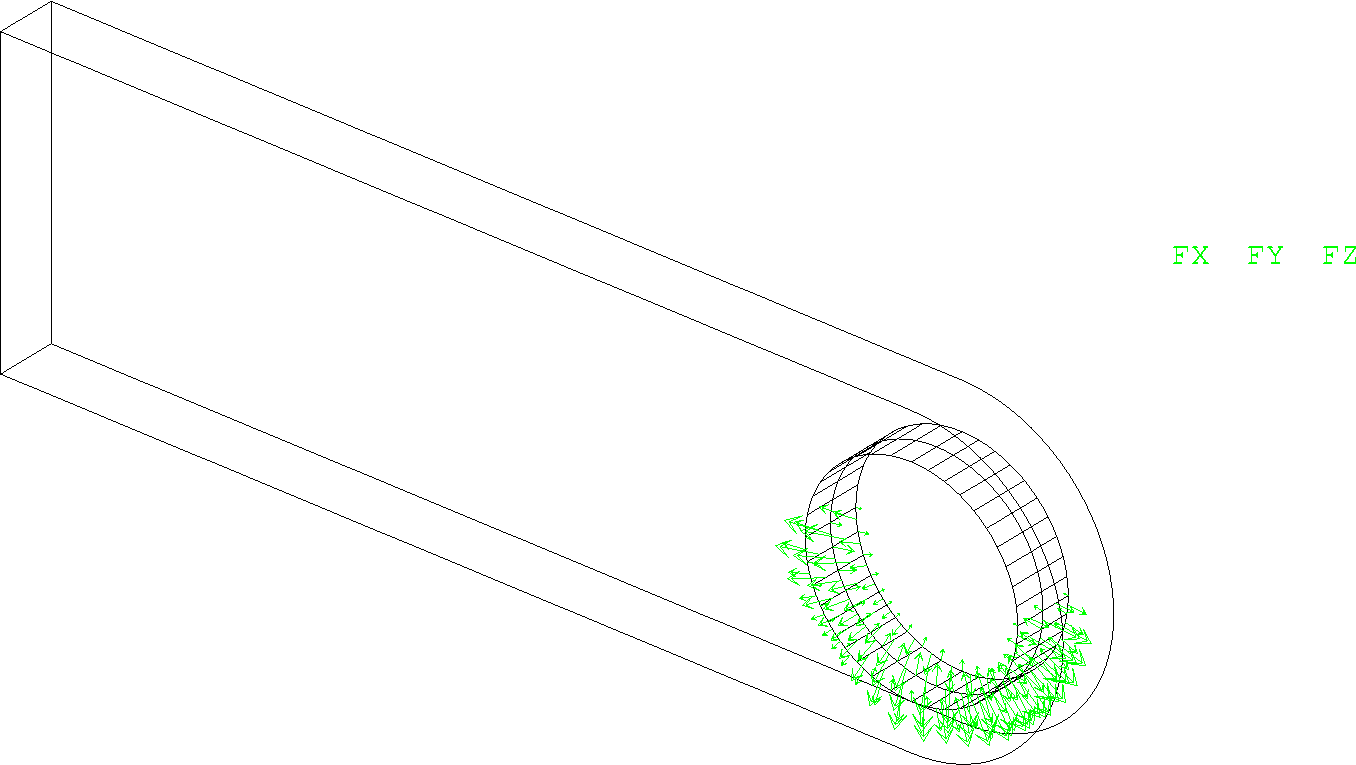
\includegraphics[width=4.5cm]{images/exo/6_forces.2}
      \end{textblock*}}
    \vspace{3cm}
    }
    \only<8-10>{
    \item \fe{3) Avec une \g{\tou{force surfacique}}}{3) With a \g{\tou{surface force}}}\\
    \begin{textblock*}{5cm}(8.7cm,-2.4cm)
      \begin{tikzpicture}
        \scriptsize
        \node[anchor=south west,inner sep=0] (image) at (0,0)
        {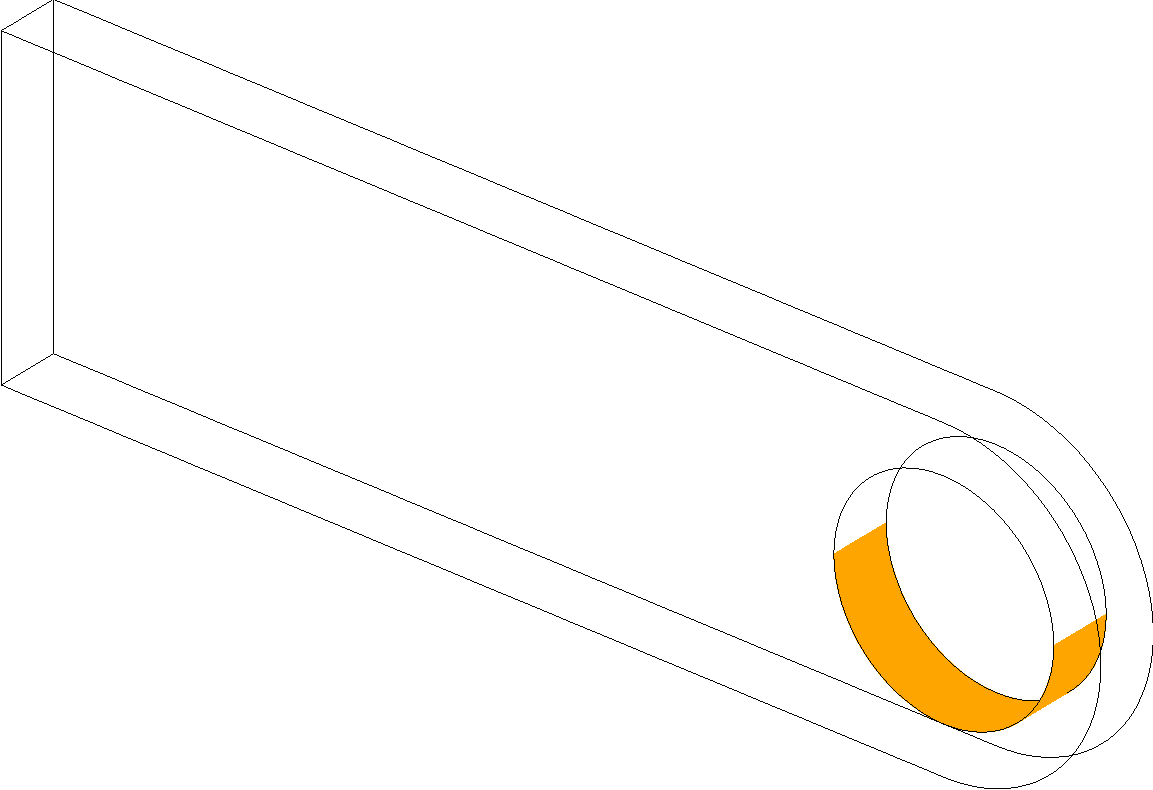
\includegraphics[width=3.5cm]{images/exo/6_cl_force}};
        \begin{scope}[x={(image.south east)},y={(image.north west)}]
          \draw (0.85,0.03) node {\orange{\kw{elmass}}};
        \end{scope}
      \end{tikzpicture}
    \end{textblock*}
    \avous{\fe{Appliquer une force surfacique (voir : FSUR 'MASS')}
              {Apply a surface force (see: FSUR 'MASS')}}
    \onslide<9-10>{
      \lstinputlisting[language=gibiane, firstline=112, lastline=112]{dgibi/formation_debutant_3_mecanique.dgibi}}
    \onslide<10>{
      \lstinputlisting[language=gibiane, firstline=113, lastline=113]{dgibi/formation_debutant_3_mecanique.dgibi}
      \lstinputlisting[language=gibiane, firstline=115, lastline=115]{dgibi/formation_debutant_3_mecanique.dgibi}
      \begin{textblock*}{5cm}(7.8cm,-0.5cm)
        \includegraphics[width=4.5cm]{images/exo/6_forces.3}
      \end{textblock*}}
    \vspace{5cm}
    }
  \end{itemize}
\end{frame}

\begin{frame}{\fe{6 Mécanique linéaire}{6 Linear mechanics}}
             {\fe{Élasticité}{Elasticity}}
  \begin{itemize}
    \item \fe{Résolution des 3 cas de chargement}{Solving 3 load cases}
    \lstinputlisting[basicstyle=\ttfamily\tiny, language=gibiane, firstline=125, lastline=127]{dgibi/formation_debutant_3_mecanique.dgibi}
    \item<2->\fe{Tracé des déformées}{Plotting the deformed shapes}
    \onslide<2->{
      \lstinputlisting[basicstyle=\ttfamily\tiny, language=gibiane, firstline=129, lastline=132]{dgibi/formation_debutant_3_mecanique.dgibi}}
    \onslide<3->{
      \lstinputlisting[basicstyle=\ttfamily\tiny, language=gibiane, firstline=137, lastline=139]{dgibi/formation_debutant_3_mecanique.dgibi}}
    \onslide<3>{
      \begin{textblock*}{5cm}(8.7cm,-6.2cm)
        \includegraphics[width=3.6cm]{images/exo/6_deformees.1}
      \end{textblock*}
      \begin{textblock*}{5cm}(8.7cm,-3.4cm)
        \includegraphics[width=3.6cm]{images/exo/6_deformees.2}
      \end{textblock*}
      \begin{textblock*}{5cm}(8.7cm,-0.6cm)
        \includegraphics[width=3.6cm]{images/exo/6_deformees.3}
      \end{textblock*}}
    \onslide<4->{
      \lstinputlisting[basicstyle=\ttfamily\tiny, language=gibiane, firstline=141, lastline=143]{dgibi/formation_debutant_3_mecanique.dgibi}
      \lstinputlisting[basicstyle=\ttfamily\tiny, language=gibiane, firstline=145, lastline=145]{dgibi/formation_debutant_3_mecanique.dgibi}
      \begin{textblock*}{5.5cm}(6.5cm,-3cm)
        \includegraphics[width=5.5cm]{images/exo/6_deformees.4}
      \end{textblock*}}
  \end{itemize}
\end{frame}

\begin{frame}{\fe{6 Mécanique linéaire}{6 Linear mechanics}}
             {\fe{Élasticité}{Elasticity}}
  \begin{itemize}
    \item \fe{Forces de réaction}{Reaction forces}
    \lstinputlisting[basicstyle=\ttfamily\tiny, language=gibiane, firstline=148, lastline=150]{dgibi/formation_debutant_3_mecanique.dgibi}
    \lstinputlisting[basicstyle=\ttfamily\tiny, language=gibiane, firstline=155, lastline=155]{dgibi/formation_debutant_3_mecanique.dgibi}
    \begin{textblock*}{5cm}(7.4cm,-2.5cm)
      \includegraphics[width=5cm]{images/exo/6_reactions}
    \end{textblock*}
    \item<2->\fe{Déformations et contraintes}{Strains and stresses}
    \onslide<2->{
      \lstinputlisting[basicstyle=\ttfamily\tiny, language=gibiane, firstline=158, lastline=162]{dgibi/formation_debutant_3_mecanique.dgibi}
      \lstinputlisting[basicstyle=\ttfamily\tiny, language=gibiane, firstline=167, lastline=167]{dgibi/formation_debutant_3_mecanique.dgibi}}
    \onslide<2>{
      \begin{textblock*}{5cm}(7.4cm,-2cm)
        \includegraphics[width=5cm]{images/exo/6_contraintes.1.pdf}
      \end{textblock*}}
    \onslide<3>{
      \begin{textblock*}{5cm}(7.4cm,-2cm)
        \includegraphics[width=5cm]{images/exo/6_contraintes.2.pdf}
      \end{textblock*}}
    \onslide<3->{
      \lstinputlisting[basicstyle=\ttfamily\tiny, language=gibiane, firstline=169, lastline=169]{dgibi/formation_debutant_3_mecanique.dgibi}
      \lstinputlisting[basicstyle=\ttfamily\tiny, language=gibiane, firstline=171, lastline=171]{dgibi/formation_debutant_3_mecanique.dgibi}
      \vspace{0.5cm}
      \item[]<3-> \violet{\emph{\fe{Nouvel objet : DEFORMEE}{New object: DEFORMEE}}}}
  \end{itemize}
\end{frame}

\begin{frame}{\fe{6 Mécanique linéaire}{6 Linear mechanics}}
             {\fe{Élasticité}{Elasticity}}
  \begin{itemize}
    \item \fe{Contrainte de von Mises}{von Mises stress}
    \lstinputlisting[basicstyle=\ttfamily\tiny, language=gibiane, firstline=174, lastline=176]{dgibi/formation_debutant_3_mecanique.dgibi}
    \lstinputlisting[basicstyle=\ttfamily\tiny, language=gibiane, firstline=178, lastline=178]{dgibi/formation_debutant_3_mecanique.dgibi}
    \begin{textblock*}{5cm}(7.4cm,-4cm)
      \includegraphics[width=5cm]{images/exo/6_contraintes.3.pdf}
    \end{textblock*}
    \onslide<2->{
      \lstinputlisting[basicstyle=\ttfamily\tiny, language=gibiane, firstline=180, lastline=180]{dgibi/formation_debutant_3_mecanique.dgibi}
      \lstinputlisting[basicstyle=\ttfamily\tiny, language=gibiane, firstline=182, lastline=182]{dgibi/formation_debutant_3_mecanique.dgibi}
      \begin{textblock*}{5cm}(7.4cm,-1.1cm)
        \includegraphics[width=5cm]{images/exo/6_contraintes.4.pdf}
      \end{textblock*}}
  \end{itemize}
\end{frame}

\begin{frame}{\fe{6 Mécanique linéaire}{6 Linear mechanics}}
             {\fe{Élasticité}{Elasticity}}
  \begin{itemize}
    \item \fe{Évolution d'un champ le long d'une ligne\\
              du maillage}
             {Field evolution along a line of the mesh\\~}
    \lstinputlisting[basicstyle=\ttfamily\tiny, language=gibiane, firstline=185, lastline=188]{dgibi/formation_debutant_3_mecanique.dgibi}
    \lstinputlisting[basicstyle=\ttfamily\tiny, language=gibiane, firstline=193, lastline=193]{dgibi/formation_debutant_3_mecanique.dgibi}
    \begin{textblock*}{5cm}(8.1cm,-2.7cm)
      \includegraphics[width=4cm]{images/exo/6_evol_contraintes.1}
    \end{textblock*}
    \item<2->\fe{Évolution d'un champ le long d'une ligne\\
                 quelconque}
                {Field evolution along any line\\~}
    \onslide<2->{
      \lstinputlisting[basicstyle=\ttfamily\tiny, language=gibiane, firstline=196, lastline=202]{dgibi/formation_debutant_3_mecanique.dgibi}
      \lstinputlisting[basicstyle=\ttfamily\tiny, language=gibiane, firstline=204, lastline=204]{dgibi/formation_debutant_3_mecanique.dgibi}
      \begin{textblock*}{5cm}(8.6cm,-3.3cm)
        \includegraphics[width=3cm]{images/exo/6_evol_contraintes.2}
      \end{textblock*}}
    \onslide<3->{
      \lstinputlisting[basicstyle=\ttfamily\tiny, language=gibiane, firstline=206, lastline=208]{dgibi/formation_debutant_3_mecanique.dgibi}
      \lstinputlisting[basicstyle=\ttfamily\tiny, language=gibiane, firstline=210, lastline=210]{dgibi/formation_debutant_3_mecanique.dgibi}
      \begin{textblock*}{5cm}(8.1cm,-2.7cm)
        \includegraphics[width=4cm]{images/exo/6_evol_contraintes.3}
      \end{textblock*}}
  \end{itemize}
\end{frame}





\fe{\subsection{Thermo Mécanique linéaire}}{\subsection{Linear Thermo Mechanics}}
\begin{frame}{\fe{7 Problème étudié}{7 Problem description}}
  \begin{itemize}
    \item \gray{\fe{Élasticité linéaire}{Linear elasticity}}
    \begin{columns}
      \begin{column}{.4\textwidth}
        \item \gray{\fe{Déplacements imposés}{Imposed displacements}}
        \footnotesize
        \begin{tikzpicture}
          \node[anchor=south west,inner sep=0,opacity=0.3] (image) at (0,0)
          {\includegraphics[width=3.5cm]{images/exo/6_cl_deplacement}};
          \begin{scope}[x={(image.south east)},y={(image.north west)},color=violet,opacity=0.3]
            \draw (0.06,0.7) node[anchor=north west] {$u_x=u_y=u_z$~=~0~m};
          \end{scope}
        \end{tikzpicture}
        \normalsize
      \end{column}
      \begin{column}{.4\textwidth}
        \item \gray{\fe{Forces imposées}{Imposed forces}}
        \footnotesize
        \begin{tikzpicture}
          \node[anchor=south west,inner sep=0,opacity=0.3] (image) at (0,0)
          {\includegraphics[width=3.5cm]{images/exo/6_cl_force}};
          \begin{scope}[x={(image.south east)},y={(image.north west)},color=orange,opacity=0.3]
            \draw (0.8,0.75) node[anchor=north west] {\fe{masse suspendue}{hanging mass}};
            \draw (0.9,0.6) node[anchor=north west] {$m$~=~2500~kg};
          \end{scope}
        \end{tikzpicture}
        \normalsize
      \end{column}
    \end{columns}
    \begin{columns}
      \begin{column}{.4\textwidth}
        \item \fe{\tou{Chargement thermique}}{\tou{Thermal load}}
        \footnotesize
        \begin{tikzpicture}
          \node[anchor=south west,inner sep=0] (image) at (0,0)
          {\includegraphics[width=4cm]{images/exo/2.2_temperatures}};
          \begin{scope}[x={(image.south east)},y={(image.north west)},color=blue]
            \draw (0.1,0.2) node {dilatation};
            \draw (0.1,0.05) node {$\alpha$~=~10$^{-5}$~K$^{-1}$};
          \end{scope}
        \end{tikzpicture}
        \normalsize
      \end{column}
      \begin{column}{.4\textwidth}
      \end{column}
    \end{columns}
  \end{itemize}
\end{frame}

\begin{frame}{\fe{7 Mécanique linéaire}{7 Linear mechanics}}
             {\fe{Élasticité, chargement thermique}{Elasticity, thermal load}}
  \begin{itemize}
    \item \fe{Prise en compte de la dilatation thermique}
             {Taking thermal expansion into account}
    \begin{equation*}
      \int_{V}[B]^T\{\sigma\}dV=\{F\}
    \end{equation*}
    \begin{equation*}
      \int_{V}[B]^T[C]\{\varepsilon-\green{\varepsilon_{\tx{th}}}\}dV=\{F\}
    \end{equation*}
    \begin{equation*}
      \int_{V}[B]^T[C]\{\varepsilon\}dV=\{F\}+\green{\int_{V}[B]^T[C]\{\varepsilon\}_{\tx{th}}dV}
    \end{equation*}
    \begin{equation*}
      [K]\{U\}=\{F\}+\green{\underbrace{\int_{V}[B]^T[C]\{\varepsilon\}_{\tx{th}}dV}_{\{F\}_{\tx{th}}}}
    \end{equation*}
  \end{itemize}
\end{frame}

\begin{frame}{\fe{7 Mécanique linéaire}{7 Linear mechanics}}
             {\fe{Élasticité, chargement thermique}{Elasticity, thermal load}}
  \begin{itemize}
    \item \fe{Objectif : calcul mécanique linéaire précédent\\
              \tou{avec un chargement thermique supplémentaire}}
            {Objective: previous linear mechanical calculation\\
             \tou{with an additional thermal load}}
    \begin{equation*}
      [K]\{U\}=\{F\}+\green{\underbrace{\int_{V}[B]^T[C]\{\varepsilon\}_{\tx{th}}dV}_{\{F\}_{\tx{th}}}}
    \end{equation*}
    \item \fe{Méthode :}{Method:}\\
    \begin{tabular}{ll}
      \fe{déformations thermiques}{thermal strains} & $\green{\{\varepsilon\}_{\tx{th}}}$\\
      \fe{contraintes thermiques}{thermal stresses} & $\green{\{\sigma\}_{\tx{th}}=[C]\{\varepsilon\}_{\tx{th}}}$\\
      \fe{forces nodales éq.}{nodal eq. forces} & $\green{\{F\}_{\tx{th}}=\int_{V}[B]^T\{\sigma\}_{\tx{th}}dV}$\\
      \fe{résolution avec \kwr{RESO}}{sovling with \kwr{RESO}} & $\{U\}=[K]^{-1}(\{F\}+\green{\{F\}_{\tx{th}}})$
    \end{tabular}
  \end{itemize}
\end{frame}

\begin{frame}{\fe{7 Mécanique linéaire}{7 Linear mechanics}}
             {\fe{Élasticité, chargement thermique}{Elasticity, thermal load}}
  \begin{itemize}
    \item \fe{Déformation thermique}{Thermal strain}
    \lstinputlisting[language=gibiane, firstline=229, lastline=232]{dgibi/formation_debutant_3_mecanique.dgibi}
    \begin{flushright}
      \footnotesize
      $\{\varepsilon\}_{\tx{th}}=\alpha\{\Delta T\}$
      \normalsize
    \end{flushright}
    \item \fe{Pseudo contraintes thermique}{Pseudo thermal stresses}
    \lstinputlisting[language=gibiane, firstline=234, lastline=235]{dgibi/formation_debutant_3_mecanique.dgibi}
    \begin{flushright}
      \footnotesize
      $\{\sigma\}_{\tx{th}}=[C]\{\varepsilon\}_{\tx{th}}$
      \normalsize
    \end{flushright}
    \item \fe{Forces nodale équivalentes}{Nodal equivalent forces}
    \lstinputlisting[language=gibiane, firstline=237, lastline=239]{dgibi/formation_debutant_3_mecanique.dgibi}
    \begin{flushright}
      \footnotesize
      $\{F\}_{\tx{th}}=\int_{V}[B]^T\{\sigma\}_{\tx{th}}dV$
      \normalsize
    \end{flushright}
  \end{itemize}
\end{frame}

\begin{frame}{\fe{7 Mécanique linéaire}{7 Linear mechanics}}
             {\fe{Élasticité, chargement thermique}{Elasticity, thermal load}}
  \begin{itemize}
    \item \fe{Résolution et affichage des résultats}{Solving and plotting results}
    \lstinputlisting[language=gibiane, firstline=241, lastline=246]{dgibi/formation_debutant_3_mecanique.dgibi}
    \lstinputlisting[language=gibiane, firstline=251, lastline=251]{dgibi/formation_debutant_3_mecanique.dgibi}
    \begin{textblock*}{5cm}(8.2cm,-3.8cm)
      \includegraphics[width=4cm]{images/exo/7_deformee}
    \end{textblock*}
    \onslide<2->{
      \lstinputlisting[language=gibiane, firstline=254, lastline=257]{dgibi/formation_debutant_3_mecanique.dgibi}
      \lstinputlisting[language=gibiane, firstline=262, lastline=262]{dgibi/formation_debutant_3_mecanique.dgibi}
      \begin{textblock*}{5cm}(7.2cm,-2.5cm)
        \includegraphics[width=5cm]{images/exo/7_contraintes.pdf}
      \end{textblock*}}
  \end{itemize}
\end{frame}

\begin{frame}{\fe{8 Problème étudié}{8 Problem description}}
  \begin{itemize}
    \item \gray{\fe{Élasticité linéaire}{Linear elasticity}}
    \begin{columns}
      \begin{column}{.4\textwidth}
        \item \gray{\fe{Déplacements imposés}{Imposed displacements}}
        \footnotesize
        \begin{tikzpicture}
          \node[anchor=south west,inner sep=0,opacity=0.3] (image) at (0,0)
          {\includegraphics[width=3.5cm]{images/exo/6_cl_deplacement}};
          \begin{scope}[x={(image.south east)},y={(image.north west)},color=violet,opacity=0.3]
            \draw (0.06,0.7) node[anchor=north west] {$u_x=u_y=u_z$~=~0~m};
          \end{scope}
        \end{tikzpicture}
        \normalsize
      \end{column}
      \begin{column}{.4\textwidth}
        \item \gray{\fe{Forces imposées}{Imposed forces}}
        \footnotesize
        \begin{tikzpicture}
          \node[anchor=south west,inner sep=0,opacity=0.3] (image) at (0,0)
          {\includegraphics[width=3.5cm]{images/exo/6_cl_force}};
          \begin{scope}[x={(image.south east)},y={(image.north west)},color=orange,opacity=0.3]
            \draw (0.8,0.75) node[anchor=north west] {\fe{masse suspendue}{hanging mass}};
            \draw (0.9,0.6) node[anchor=north west] {$m$~=~2500~kg};
          \end{scope}
        \end{tikzpicture}
        \normalsize
      \end{column}
    \end{columns}
    \begin{columns}
      \begin{column}{.4\textwidth}
        \item \fe{Chargement thermique}{Thermal load}
        \footnotesize
        \begin{tikzpicture}
          \node[anchor=south west,inner sep=0] (image) at (0,0)
          {\includegraphics[width=4cm]{images/exo/2.2_temperatures}};
          \begin{scope}[x={(image.south east)},y={(image.north west)},color=blue]
            \draw (0.1,0.2) node {dilatation};
            \draw (0.1,0.05) node {\fe{$\alpha$ \tou{hétérogène}}{$\alpha$ \tou{heterogeneous}}};
          \end{scope}
        \end{tikzpicture}
        \normalsize
      \end{column}
      \begin{column}{.4\textwidth}
      \end{column}
    \end{columns}
  \end{itemize}
\end{frame}

\begin{frame}{\fe{8 Mécanique linéaire}{8 Linear mechanics}}
             {\fe{Élasticité, chargement thermique, matériau hétérogène}
                 {Elasticity, thermal load, heterogeneous matrial}}
  \begin{itemize}
    \item \fe{Coefficient de dilatation $\alpha$ dépendant de $x$ (loi normale)}
             {Thermal expansion coefficient $\alpha$ dependent on $x$ (normal distribution)}
    \footnotesize
    \begin{equation*}
      \alpha(x)=\alpha_0\left(1+3e^{-\left(\frac{x-\mu}{\sigma}\right)^2}\right)
    \end{equation*}
    \footnotesize
    \fe{avec :}{with}
    \begin{itemize}
        \footnotesize
        \item[] $\mu=\frac{l}{2}$ \fe{moyenne}{mean value}
      \item[] $\sigma=\frac{l}{5}$ \fe{écart type}{standard deviation}
    \end{itemize}
    \normalsize
    \onslide<2->{
      \lstinputlisting[language=gibiane, firstline=281, lastline=284]{dgibi/formation_debutant_3_mecanique.dgibi}}
      \onslide<3->{
        \lstinputlisting[language=gibiane, firstline=285, lastline=287]{dgibi/formation_debutant_3_mecanique.dgibi}
        \lstinputlisting[language=gibiane, firstline=292, lastline=292]{dgibi/formation_debutant_3_mecanique.dgibi}
        \begin{textblock*}{5cm}(7.2cm,-4.6cm)
          \includegraphics[width=5cm]{images/exo/8_alpha_variable}
        \end{textblock*}}
    \end{itemize}
\end{frame}

\begin{frame}{\fe{8 Mécanique linéaire}{8 Linear mechanics}}
             {\fe{Élasticité, chargement thermique, matériau hétérogène}
                 {Elasticity, thermal load, heterogeneous matrial}}
  \begin{itemize}
    \item \fe{Mise à jour des caractéristiques matériau}
             {Updating the material properties}
    \lstinputlisting[language=gibiane, firstline=294, lastline=297]{dgibi/formation_debutant_3_mecanique.dgibi}
    \item<2->\fe{Mise à jour du chargement thermique}
                {Updating the thermal load}
    \onslide<2->{
        \lstinputlisting[language=gibiane, firstline=299, lastline=302]{dgibi/formation_debutant_3_mecanique.dgibi}}
    \end{itemize}
\end{frame}

\begin{frame}{\fe{8 Mécanique linéaire}{8 Linear mechanics}}
             {\fe{Élasticité, chargement thermique, matériau hétérogène}
                 {Elasticity, thermal load, heterogeneous matrial}}
  \begin{itemize}
    \item \fe{Résolution et affichage des résultats}{Solving and plotting results}
    \lstinputlisting[language=gibiane, firstline=304, lastline=308]{dgibi/formation_debutant_3_mecanique.dgibi}
    \lstinputlisting[language=gibiane, firstline=313, lastline=313]{dgibi/formation_debutant_3_mecanique.dgibi}
    \begin{textblock*}{5cm}(8.2cm,-3.8cm)
      \includegraphics[width=4cm]{images/exo/8_deformee}
    \end{textblock*}
    \onslide<2->{
      \lstinputlisting[language=gibiane, firstline=316, lastline=319]{dgibi/formation_debutant_3_mecanique.dgibi}
      \lstinputlisting[language=gibiane, firstline=324, lastline=324]{dgibi/formation_debutant_3_mecanique.dgibi}
      \begin{textblock*}{5cm}(7.2cm,-2.5cm)
        \includegraphics[width=5cm]{images/exo/8_contraintes.pdf}
      \end{textblock*}}
  \end{itemize}
\end{frame}




\fe{\subsection{Thermo mécanique non linéaire}}{\subsection{Non Linear Thermo Mechanics}}
\begin{frame}{\fe{9.1 Problème étudié}{9.1 Problem description}}
  \begin{itemize}
    \item \fe{\tou{Élasto plasticité} (plasticité parfaite)}
             {\tou{Elasto plasticity} (perfect plasticity)}
    \begin{textblock*}{5cm}(8.1cm,-1.8cm)
      \begin{tikzpicture}
        % axes
        \draw [<->,thick] (0,2) node (yaxis) [above] {$\sigma$}
                       |- (3,0) node (xaxis) [right] {$\varepsilon$};
        % courbe de traction
        \draw (0,0) -- (1,1.5) coordinate (a) -- (2.5,1.5);
        % ligne pour sigy
        \draw[dashed] (yaxis |- a) node[left] {$\sigma_y$} -| (a) ;
      \end{tikzpicture}
    \end{textblock*}
    \begin{center}
    \footnotesize
    \begin{tikzpicture}
      \node[anchor=south west,inner sep=0] (image) at (0,0)
      {\includegraphics[width=4cm]{images/exo/1.2_geometrie}};
      \begin{scope}[x={(image.south east)},y={(image.north west)}]
        \draw (1,0.9) node[anchor=west] {$E$~=~200~GPa};
        \draw (1,0.7) node[anchor=west] {$\nu$~=~0.3};
        \draw (1,0.5) node[anchor=west] {$\alpha(x)=10^{-5}\left(1+3e^{-\left(\frac{x-\mu}{\sigma}\right)^2}\right)$~K$^{-1}$};
        \draw (1,0.3) node[anchor=west] {\tou{$\sigma_y$~=~250~MPa}};
      \end{scope}
    \end{tikzpicture}
    \normalsize
    \end{center}
    \begin{columns}
      \begin{column}{.4\textwidth}
        \item \gray{\fe{Déplacements imposés}{Imposed displacements}}
      \end{column}
      \begin{column}{.4\textwidth}
        \item \gray{\fe{Forces imposées}{Imposed forces}}
      \end{column}
    \end{columns}
    \begin{columns}
      \begin{column}{.4\textwidth}
        \item \gray{\fe{Chargement thermique}{Thermal load}}
      \end{column}
      \begin{column}{.4\textwidth}
      \end{column}
    \end{columns}
  \end{itemize}
\end{frame}

\begin{frame}{\fe{9.1 Mécanique non linéaire}{9.1 Non linear mechanics}}
             {\fe{Élastoplasticité, chargement thermique, matériau hétérogène}
                 {Elastoplasticity, thermal load, heterogeneous matrial}}
  \begin{itemize}
    \item \fe{Objectif : calcul mécanique \tou{non linéaire} (matériau)}
             {Objective: \tou{non linear} mechanical calculation}
    \begin{equation*}
      \int_{V}[B]^T\{\sigma\}dV=\{F\}
    \end{equation*}
    \item \fe{Méthode :}{Method:}\\
    \begin{tabular}{ll}
      \fe{ajout d'un modèle de plasticité}{adding a plastic model}\\
      \fe{description temporelle des chargements (pseudo temps)}{time description of loads (pseudo time)}\\
      \fe{résolution avec la procédure \kwo{PASAPAS}}{using the \kwo{PASAPAS} solving procedure}\\
    \end{tabular}
  \end{itemize}
\end{frame}

\begin{frame}{\fe{9.1 Mécanique non linéaire}{9.1 Non linear mechanics}}
             {\fe{Élastoplasticité, chargement thermique, matériau hétérogène}
                 {Elastoplasticity, thermal load, heterogeneous matrial}}
  \begin{itemize}
    \item \fe{Formulation mathématique (élasticité)}{Mathematical formulation (elasticity)}
    \lstinputlisting[basicstyle=\ttfamily\tiny, language=gibiane, firstline=46, lastline=46]{dgibi/formation_debutant_3_mecanique.dgibi}
    \lstinputlisting[basicstyle=\ttfamily\tiny, language=gibiane, firstline=343, lastline=347]{dgibi/formation_debutant_3_mecanique.dgibi}
    \item<2->\fe{Chargements : description temporelle}{Loads: time description}
    \lstinputlisting[basicstyle=\ttfamily\tiny, language=gibiane, firstline=351, lastline=353]{dgibi/formation_debutant_3_mecanique.dgibi}
    \lstinputlisting[basicstyle=\ttfamily\tiny, language=gibiane, firstline=354, lastline=361]{dgibi/formation_debutant_3_mecanique.dgibi}
    \end{itemize}
\end{frame}

\begin{frame}{\fe{9.1 Mécanique non linéaire}{9.1 Non linear mechanics}}
             {\fe{Élastoplasticité, chargement thermique, matériau hétérogène}
                 {Elastoplasticity, thermal load, heterogeneous matrial}}
  \begin{itemize}
    \item \fe{Résolution avec \kwo{PASAPAS}}{Solving with \kwo{PASAPAS}}\\
    \avous{\fe{Remplir la TABLE et lancer \kw{PASAPAS}}{Fill the TABLE and launch \kw{PASAPAS}}}
    \onslide<2->{
      \lstinputlisting[language=gibiane, firstline=363, lastline=371]{dgibi/formation_debutant_3_mecanique.dgibi}}
    \end{itemize}
\end{frame}

\begin{frame}{\fe{9.1 Mécanique non linéaire}{9.1 Non linear mechanics}}
             {\fe{Élastoplasticité, chargement thermique, matériau hétérogène}
                 {Elastoplasticity, thermal load, heterogeneous matrial}}
  \begin{itemize}
    \item \fe{Post traitement : boucle de tracés}{Post processing: loop for plot}
    \lstinputlisting[basicstyle=\ttfamily\tiny, language=gibiane, firstline=379, lastline=385]{dgibi/formation_debutant_3_mecanique.dgibi}
    \lstinputlisting[basicstyle=\ttfamily\tiny, language=gibiane, firstline=387, lastline=387]{dgibi/formation_debutant_3_mecanique.dgibi}
    \lstinputlisting[basicstyle=\ttfamily\tiny, language=gibiane, firstline=389, lastline=389]{dgibi/formation_debutant_3_mecanique.dgibi}
  \end{itemize}
  \begin{textblock*}{5cm}(7cm,-1cm)
    \animategraphics[controls,loop,poster=last,width=5cm]{10}{images/exo/9.1_contraintes.}{01}{21}
  \end{textblock*}
  \vspace{3cm}
\end{frame}

\begin{frame}{\fe{9.1 Mécanique non linéaire}{9.1 Non linear mechanics}}
             {\fe{Élastoplasticité, chargement thermique, matériau hétérogène}
                 {Elastoplasticity, thermal load, heterogeneous matrial}}
  \begin{itemize}
    \item \fe{Post traitement : boucle de tracés}{Post processing: loop for plot}
    \lstinputlisting[basicstyle=\ttfamily\tiny, language=gibiane, firstline=396, lastline=402]{dgibi/formation_debutant_3_mecanique.dgibi}
    \lstinputlisting[basicstyle=\ttfamily\tiny, language=gibiane, firstline=404, lastline=404]{dgibi/formation_debutant_3_mecanique.dgibi}
    \lstinputlisting[basicstyle=\ttfamily\tiny, language=gibiane, firstline=406, lastline=406]{dgibi/formation_debutant_3_mecanique.dgibi}
  \end{itemize}
  \begin{textblock*}{5cm}(7cm,-1cm)
    \animategraphics[controls,loop,poster=last,width=5cm]{10}{images/exo/9.1_variables_internes.}{01}{21}
  \end{textblock*}
  \vspace{3cm}
\end{frame}

\begin{frame}{\fe{9.2 Problème étudié}{9.2 Problem description}}
  \begin{itemize}
    \item \fe{Élasto plasticité (plasticité parfaite), \tou{dépendance à la température}}
             {Elasto plasticity (perfect plasticity), \tou{temperature dependent}}
    \begin{center}
    \footnotesize
    \begin{tikzpicture}
      \node[anchor=south west,inner sep=0] (image) at (0,0)
      {\includegraphics[width=4cm]{images/exo/1.2_geometrie}};
      \begin{scope}[x={(image.south east)},y={(image.north west)}]
        \draw (1,0.9) node[anchor=west] {$E$~=~200~GPa};
        \draw (1,0.7) node[anchor=west] {$\nu$~=~0.3};
        \draw (1,0.5) node[anchor=west] {$\alpha(x)=10^{-5}\left(1+3e^{-\left(\frac{x-\mu}{\sigma}\right)^2}\right)$~K$^{-1}$};
        \draw (1,0.3) node[anchor=west] {\tou{$\sigma_y=f(T)$}};
      \end{scope}
    \end{tikzpicture}
    \normalsize
    \end{center}
    \begin{columns}
      \begin{column}{.4\textwidth}
        \item \gray{\fe{Déplacements imposés}{Imposed displacements}}
      \end{column}
      \begin{column}{.4\textwidth}
        \item \gray{\fe{Forces imposées}{Imposed forces}}
      \end{column}
    \end{columns}
    \begin{columns}
      \begin{column}{.4\textwidth}
        \item \gray{\fe{Chargement thermique}{Thermal load}}
      \end{column}
      \begin{column}{.4\textwidth}
      \end{column}
    \end{columns}
  \end{itemize}
\end{frame}

\begin{frame}{\fe{9.2 Mécanique non linéaire}{9.2 Non linear mechanics}}
             {\fe{Élastoplasticité, chargement thermique, matériau hétérogène, T dépendant}
                 {Elastoplasticity, thermal load, heterogeneous matrial, T dependent}}
  \begin{itemize}
    \item \fe{Dépendance d'un paramètre à la température}{Temperature dependence of a parameter}
    \lstinputlisting[basicstyle=\ttfamily\tiny, language=gibiane, firstline=426, lastline=430]{dgibi/formation_debutant_3_mecanique.dgibi}
    \onslide<2->{
      \lstinputlisting[basicstyle=\ttfamily\tiny, language=gibiane, firstline=435, lastline=435]{dgibi/formation_debutant_3_mecanique.dgibi}
      \begin{textblock*}{5cm}(8.1cm,0cm)
        \includegraphics[width=4.3cm]{images/exo/9.2_evol_sigy}
      \end{textblock*}}
    \item<3->\fe{Mise à jour des caractéristiques matériau}{Updating the material properties}
    \onslide<3->{
      \lstinputlisting[basicstyle=\ttfamily\tiny, language=gibiane, firstline=438, lastline=441]{dgibi/formation_debutant_3_mecanique.dgibi}}
  \end{itemize}
\end{frame}

\begin{frame}{\fe{9.2 Mécanique non linéaire}{9.2 Non linear mechanics}}
             {\fe{Élastoplasticité, chargement thermique, matériau hétérogène, T dépendant}
                 {Elastoplasticity, thermal load, heterogeneous matrial, T dependent}}
  \begin{itemize}
    \item \fe{Résolution avec \kwo{PASAPAS}}{Solving with \kwo{PASAPAS}}
    \lstinputlisting[language=gibiane, firstline=443, lastline=451]{dgibi/formation_debutant_3_mecanique.dgibi}
  \end{itemize}
\end{frame}

\begin{frame}{\fe{9.2 Mécanique non linéaire}{9.2 Non linear mechanics}}
             {\fe{Élastoplasticité, chargement thermique, matériau hétérogène, T dépendant}
                 {Elastoplasticity, thermal load, heterogeneous matrial, T dependent}}
  \begin{itemize}
    \item \fe{Post traitement : boucle de tracés}{Post processing: loop for plot}
    \lstinputlisting[basicstyle=\ttfamily\tiny, language=gibiane, firstline=454, lastline=454]{dgibi/formation_debutant_3_mecanique.dgibi}
    \lstinputlisting[basicstyle=\ttfamily\tiny, language=gibiane, firstline=460, lastline=466]{dgibi/formation_debutant_3_mecanique.dgibi}
    \lstinputlisting[basicstyle=\ttfamily\tiny, language=gibiane, firstline=468, lastline=468]{dgibi/formation_debutant_3_mecanique.dgibi}
    \lstinputlisting[basicstyle=\ttfamily\tiny, language=gibiane, firstline=470, lastline=470]{dgibi/formation_debutant_3_mecanique.dgibi}
    \lstinputlisting[basicstyle=\ttfamily\tiny, language=gibiane, firstline=474, lastline=474]{dgibi/formation_debutant_3_mecanique.dgibi}
  \end{itemize}
  \begin{textblock*}{5cm}(7cm,-1.4cm)
    \animategraphics[controls,loop,poster=last,width=5cm]{10}{images/exo/9.2_variables_internes.}{01}{21}
  \end{textblock*}
  \vspace{3cm}
\end{frame}

%%%%%%%%%%%%%%%%%%%%%%%%%%%%%%%%%%%%%%%%%%%%%%%%%%%%%%%%%%%%%%
\fe{\section{Compléments}}{\section{Supplements}}
\label{complements}
%%%%%%%%%%%%%%%%%%%%%%%%%%%%%%%%%%%%%%%%%%%%%%%%%%%%%%%%%%%%%%

\begin{frame}{\fe{Fichiers solution}{solution files}}
  \begin{itemize}
  \item \fe{Les fichiers solution de cette formation sont des cas tests\\
            téléchargeables sur le site web :}
           {The solution files of this tutorial are in the examples base\\
            download them from the web site:}\\~\\
        \url{http://www-cast3m.cea.fr/index.php?page=exemples}\\~\\
  $\Rightarrow$~formation\_debutant\_1\_maillage.dgibi\\
  $\Rightarrow$~formation\_debutant\_2\_thermique.dgibi\\
  $\Rightarrow$~formation\_debutant\_3\_mecanique.dgibi
  \end{itemize}
\end{frame}



\end{document}
